\documentclass[a4paper]{report}

\usepackage{amsmath,amssymb,stmaryrd,latexsym}
\usepackage{titlepic}
%\usepackage{syntax}
\usepackage{alltt}
\usepackage{graphicx}   % Including Graphics
\usepackage{bcprules}   % Benjamin Pierce's Proof Rule Package
\usepackage{semabbrev} 
%\usepackage{verbatim} 
\usepackage{spverbatim}
\usepackage{alltt} 
\usepackage{xspace} 
\usepackage{listings} 
\usepackage{ifthen}
\usepackage{adjustbox}
\usepackage{xhfill}% http://ctan.org/pkg/xhfill
%\usepackage{color}
\usepackage[multiple]{footmisc}
\usepackage{algorithm}
\usepackage{algpseudocode}
\usepackage{grammar-defns}

\newboolean{devel}
\setboolean{devel}{false}

%\lstset{aboveskip=2\medskipamount}
%\lstset{belowskip=1.5\medskipamount}
%\lstset{abovecaptionskip=\medskipamount}
\lstdefinelanguage{hocl}{keywords={node,graph,val,actor,fun,struct,let,in,out,param,end,wire},morecomment=[l]{--}}
\lstset{language=hocl}
%\lstset{frame=single}
\lstset{frameround=tttt} 
\lstset{captionpos=t}
\lstset{breaklines=true}
%\lstset{basicstyle=\small}

%\renewcommand\lstlistingname{Example}

%%% Better hyphenation:
%\sloppy
\setlength{\topmargin}{0pt}
\setlength{\oddsidemargin}{0pt}
\setlength{\textheight}{600pt}
\setlength{\textwidth}{448pt}

%\Newcommand{\docdate}{\today} %%%!!!!

\newcommand{\version}{1.0a}
%\ifthenelse{\boolean{devel}}{\newcommand{\version}{1.3}}{\newcommand{\version}{1.1}}
%% This has to be fixed !

\newcommand{\ie}{\emph{i.e.}\xspace}
\newcommand{\txt}[1]{\hbox{#1}}
\newcommand{\emtxt}[1]{\hbox{\em{#1}}}
\newcommand{\bftxt}[1]{\hbox{\bf{#1}}}
\ifthenelse{\boolean{devel}}{\newcommand{\note}[1]{\marginpar{\tiny #1}}}{\newcommand{\note}[1]{}}
\newcommand{\todo}[1]{\note{TODO: #1}}
\ifthenelse{\boolean{devel}}{\newcommand{\tbw}[1]{$\spadesuit$ {\bf To be written\ldots}\xspace}}{\newcommand{\tbw}[1]{}}
\ifthenelse{\boolean{devel}}{\newcommand{\tbc}[1]{$\spadesuit$ {\bf To be continued\ldots}\xspace}}{\newcommand{\tbc}[1]{}}

\newcommand{\hocl}{HoCL\xspace}
\newcommand{\ocaml}{{\sc Objective Caml}\xspace}

\newenvironment{example}{\medskip\noindent{\it Example :}\begin{alltt}}{\end{alltt}}
%\newenvironment{caphexample}{\begin{lstlisting}}{\end{lstlisting}}

\algnewcommand\algorithmicforeach{\textbf{for each}}
\algdef{S}[FOR]{ForEach}[1]{\algorithmicforeach\ #1\ \algorithmicdo}


\title{HoCL Manual - \version}

\author{J. S\'erot}%\footnote{Universit\'e Clermont Auvergne, Clermont-Ferrand, France; %\texttt{jocelyn.serot@uca.fr}}}

\titlepic{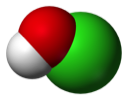
\includegraphics[width=0.25\textwidth]{figs/hocl-logo}}
\date{}

\begin{document}

\maketitle

\tableofcontents

% %%%%%%%%%%%%%%%%%%%%%%%%%%%%%%%%%%%%%%%%%%%%%%%%%%%%%%%%%%%%%%%%%%%%%%%%%%%%%%%%%%%%%%%%%
%%                                                                                     %%
%%                This file is part of the HoCL Compiler distribution                  %%
%%                                                                                     %%
%%      Copyright 2019 Jocelyn SEROT (jocelyn.serot@uca.fr).  All rights reserved.     %%
%%         This file is distributed under the terms of the MIT Library License         %%
%%                                                                                     %%
%%%%%%%%%%%%%%%%%%%%%%%%%%%%%%%%%%%%%%%%%%%%%%%%%%%%%%%%%%%%%%%%%%%%%%%%%%%%%%%%%%%%%%%%%

\chapter{Introduction}
\label{chap:intro}

This document is a short introduction to the \hocl programming language. \hocl is ... TBW

\medskip This report is structured as follows:  TBW

% the remainder of this chapter provides motivation and
% general background; Chapter~\ref{chap:overview} is an overview of the \caph language design,
% including informal descriptions of the expression, network and actor sub-languages. The full
% concrete syntax is given in chapter~\ref{chap:syntax} and the abstract syntax of the core language
% in chapter~\ref{chap:abssyn}. Chapter~\ref{chap:typing} gives the formal typing rules for \caph
% programs. Chapter~\ref{chap:static} gives the formal static semantics,
% \emph{i.e.} the interpretation of \caph programs as \emph{data-flow graphs}.
% Chapter~\ref{chap:dynamic-semantics} gives the formal dynamic semantics, which provides a way to
% \emph{simulate} \caph programs.  Chapter~\ref{chap:interm-repr} describes
%   the intermediate representation of \caph programs used as an input for the back-end code
%   generators. Chapter~\ref{cha:using-caph-compiler} describes, pragmatically, how to use the
% compiler in order to obtain graphical representations of programs, simulate them or invoke the
% SystemC or VHDL backend in order to generate code. Chapter~\ref{cha:stdlib} gives the contents of
% some ``standard libraries''. Chapter~\ref{cha:foreign-funct-interf} describes
% the mechanism by which existing C or VHDL functions can be used by \caph
% programs. Chapter~\ref{cha:compiler-options} is a summary of compiler options.
%  Chapter~\ref{cha:variants-impl} is a short, technical, overview of how \emph{variant
%   types} (described in chapter~\ref{chap:overview}) are implemented in SystemC and VHDL. 

\clearpage

\section{Motivation, goals and principles}

TBW

\begin{itemize}
\item describing dataflow process networks in an implementation-independant way (s/w, h/w, both...)
\item replace tedious GUI-based specification by a purely textual description, amenable to
  \begin{itemize}
  \item verification (by means of type-checking)
  \item abstraction
  \item versionning
  \item \ldots
  \end{itemize}
\item does not deal with the specification of individual actor behavior (actors are viewed as black
  boxes\footnote{Except for their prod-cons rates in the case of SDF actors}
\item backends for specific implementation-specific tools (ex: \textsc{preesm})
\item can be viewed as a special case of a \emph{coordination language} taking advantage of the
  natural duality between dataflow networks and functional programming languages
\end{itemize}


%%% Local Variables: 
%%% mode: latex
%%% TeX-master: "hocl"
%%% End: 

% %%%%%%%%%%%%%%%%%%%%%%%%%%%%%%%%%%%%%%%%%%%%%%%%%%%%%%%%%%%%%%%%%%%%%%%%%%%%%%%%%%%%%%%%%
%%                                                                                     %%
%%                This file is part of the HoCL Compiler distribution                  %%
%%                                                                                     %%
%%      Copyright 2019 Jocelyn SEROT (jocelyn.serot@uca.fr).  All rights reserved.     %%
%%         This file is distributed under the terms of the MIT Library License         %%
%%                                                                                     %%
%%%%%%%%%%%%%%%%%%%%%%%%%%%%%%%%%%%%%%%%%%%%%%%%%%%%%%%%%%%%%%%%%%%%%%%%%%%%%%%%%%%%%%%%%

\section{Example 1}
\label{sec:example-1}

Introduce the core idea : representing actors by \emph{functions} are wires (edges) by functional
application.

Consider the very simple DFPN depicted on Fig. xx :

\begin{verbatim}
+---+    +---+    +---+
| f |--->| g |--->| h |
+---+ x  +---+    +---+
\end{verbatim}

First formulation :
Forget about the actor declarations for the moment.

\begin{lstlisting}
let x = f ();
let y = g x;
let () = h y;
\end{lstlisting}

The \verb|let| keyword introduce \emph{network definitions}. These definitions basically say
\begin{itemize}
\item there's one instance of an actor named \verb|f|, taking no input and producing an output named
  (here) \verb|x|,
\item there's one instance of an actor named \verb|g|, taking \verb|x| as input and producing an
  output named \verb|y|,
\item there's one instance of an actor named \verb|h|, taking \verb|y| as input and producing no
  output.
\end{itemize}

Each application of an actor creates a node in the graph and the 
\emph{sharing} of the values introduced by the \verb|let| definitions (\verb|x| and \verb|y| here)
``wires'' the network by creating edges between these nodes.

\medskip
Second formulation.
Naming intermediate values (wires) is actually not necessary and we can describe the network of
Fig.XX by the following program (which is strictly equivalent to the previous one)~:

\begin{lstlisting}
let () = h (g (f ()));
\end{lstlisting}

This formulation is shorter but maybe a little bit more difficult to read because the implied number
of parenthesis (these parenthesis are required because function application, classicaly associated
to the left, so that \verb|f g x| means \verb|(f g) x| and not \verb|f (g x)|). 

\medskip
Third formulation.
With the function composition operator $o$ (denoted here \verb?||?)~:
Has a mathematical taste but still a bit unatural because functions here appears in a right-to-left
order compared to the nodes of Fig.XX.

\begin{lstlisting}
let () = (h || g || f) ();
\end{lstlisting}

\medskip
Fourth formulation.
With the special ``reverse apply'' operaror \verb|>>|, defined as \verb|x >> f = f x|~:

\begin{lstlisting}
let () = () >> f >> g >> h;
\end{lstlisting}

Because most networks will start with an actor taking \verb|()| as input, this can be further
simplified with the \verb?|>? operator, defined as \verb?f |> g = () >> f >> g?~:

\begin{lstlisting}
let () = f |> g >> h;
\end{lstlisting}

\medskip
\textbf{Note}.
A few note about the syntax~:
\begin{itemize}
\item As in most functional programming language\footnote{ML, Caml, or Haskell for example.}
  function application is denoted \emph{without parenthesis}. In other words, the applications of
  \verb|f| (resp. \verb|o|) at line 2 (resp. 3) should be read as \verb|f(x)|
  (resp. \verb|o(y)|)\footnote{And in fact, these applications can be written with
    parenthesis.}. As a special case, the application at line 1 must be viewed as the application of
  \verb|i| to a special value, denoted \verb|()| and called \verb|unit|\footnote{Similar to
    \texttt{void} in C or C++.}. 
\item Every definitions ends with a semi-colon (\verb|;|).
\end{itemize}

\medskip
How are actors defined ?

\section{Example 2}
\label{sec:example-2}

Introducing tuples. Sometimes explicit naming (binding) is required. working/simple/basic.

\section{Example 3}
\label{sec:example-3}

What about loops (feedback). Recursive wiring

\section{Example 4}
\label{sec:example-4}

Higher-order function. Where types begin to complicates ... and starts to help !

Diamond and diamonds

\section{Example 5}
\label{sec:example-5}

Graph patterns. Example with FIR. The basic HOWF (map, fold, pipe, ...).

\chapter{The \hocl language at a glance}
\label{chap:overview}

A \hocl program is composed of four distinct sets~:
\begin{itemize}
\item a set of \emph{type declarations},
\item a set of \emph{actor declarations},
\item a set of \emph{network definitions},
\item a set of \emph{pragmas}.
\end{itemize}

Each element can appear in any order in the source file, provided that precedences are met (a
declaration 

% \section{Language structure}
% \label{sec:language-struct}

% As stated in introduction, \caph is a layered language. 

% The outermost (\emph{declaration}) layer declares types, global values (constant and functions), I/O streams, actors and
% network-level objects (wires and wiring functions).
% The innermost (\emph{expression}) layer is used for describing computations. 
% An \emph{actor} sub-language is used for describing the interface and the behavior of actors and a
% \emph{network} sub-language is used for describing the structure of the dataflow process network. 

% All layers essentially share a common type system, which is presented in the next section.

% \section{Types}
% \label{sect:types}

% Broadly speaking, two categories of types can be distinguished: \emph{scalar} types and
% \emph{structured} types\footnote{The concept of \emph{type variable} is discussed separately in
%   Sec.~\ref{sec:polymorphism}}.

% \subsection{Scalar types}
% \label{sec:scalar-types}

% Scalar types are described in Table~\ref{tab:scalar-types}. They include signed and unsigned
% fixed-precision integers, booleans and floating-point values\footnote{Support of floating-point
%   values by the VHDL backend is platform-dependant (see Sec.~\ref{sec:transl-syst-vhdl}).}.

% \begin{table}
% \small
% \begin{center}
% \begin{tabular}{|l|l|} \hline
% \texttt{int} & Generic (signed) integer, range is implementation dependant\\ \hline   
% \texttt{signed<prec>} & Sized signed integer, range is $-2^{prec-1}\ldots 2^{prec-1}-1$\\ \hline   
% \texttt{unsigned<prec>} & Sized unsigned integer, range is $0 \ldots 2^{prec}-1$\\ \hline   
% \texttt{bool}       & Boolean (\verb|true|, \verb|false|) \\ \hline   
% \texttt{float}       & Floating-point value (minimal range : $-1.10^{38}\ldots+1.10^{38}$)  \\ \hline   
% \end{tabular}
% \caption{\caph scalar types}
% \label{tab:scalar-types}
% \end{center}
% \end{table}

% \medskip
% Builtin operations provided on scalar types are summarized in Table~\ref{tab:scalar-ops}.
% By \emph{builtin}, we mean the operations which
% \begin{itemize}
% \item have a runtime implementation at the simulator level,
% \item can be a automatically translated to their SystemC and VHDL equivalent by the compiler
%   back-ends\footnote{The support of floating-point values ultimately depends on the VHDL compiler.}.
% \end{itemize}

% \begin{table}
% \begin{minipage}[c]{1.0\linewidth}
% \small
% \begin{center}
% \begin{tabular}{|l|l|} \hline
% {\tt bool}      & {\tt \&\& || not} (logical and, or, not) \\ \hline 
% {\tt int}       & {\tt + - * / mod} \\ 
% {\tt signed}    & \tt {< <= = >= >} \\
% {\tt unsigned}  & \\ \hline
% {\tt signed}    & {\tt land lor lnand lnot} (bitwise operations) \\
% {\tt unsigned}  & {\tt <<}, {\tt >>} (left/right logical shift)\\  \hline
% {\tt float}     & {\tt +. -. *. /.}  \\
%                 & {\tt =. !=. <. >. <=. >=.}  \\ \hline
% %                & {\tt sll srl}\footnote{These operators can also be written {\tt <<} and {\tt >>} resp.} (left/right logical shift)\\ 
% %                & {\tt sla sra} (left/right arithmetic shift)\\ 
% %                & {\tt rol ror} (left/right rotate) \\ \hline
% \end{tabular}
% \caption{Builtin operations on scalar types}
% \label{tab:scalar-ops}
% \end{center}
% \end{minipage}
% \end{table}
% \normalsize

% % For \texttt{word}, {\verb+ & | ^ ~+} are bitwise and, inclusive or, exclusive or
% % and negation respectively.  The {\tt <<} and {\tt >>} operations pad to right/left with
% % {\tt 0}s respectively, as required.

% \subsection{Structured types}
% \label{sec:structured-types}

% Two categories of structured types are currently supported : arrays and variants.

% \bigskip \textbf{Arrays} are indexed collections of values of the same type. The corresponding type,
% \texttt{array}, is predefined in \caph. Arrays can have one, two or three dimensions~:
% \begin{itemize}
% \item for 1D arrays, each item has a scalar type,
% \item 2D arrays are viewed as arrays of 1D arrays\footnote{And for this reason, sometimes called
%     1D$\times$1D arrays.},
% \item 3D arrays are viewed as arrays of 2D arrays\footnote{And for this reason, sometimes called
%     1D$\times$1D$\times$1D arrays.}.
% \end{itemize}
% For each dimension, the size $S$ is fixed and must defined at the declaration. Indexes range from
% $0$ to $S-1$.

% Arrays can be declared either as global constants or as local variables in actors
% (Table~\ref{tab:array-decls}). In the first case, the (immutable) value of the array is part of the
% declaration and an optional type signature can be used to refine the type of the array items. In the
% second case, the type signature is not optional but the initial value can be omitted\footnote{It is
%   the progammer's responsability, of course, to ensure that no element of the array will be accessed
%   before having been properly initialized.}.  Two syntaxes -- extension and comprehension -- are
% provided for specifying initilisation values. 

% \begin{table}
% \begin{minipage}[c]{1.0\linewidth}
% \small
% \begin{center}
% \begin{tabular}{|l|r|} \hline
% \texttt{const <id> "=" <array\_init> [ ":" <array\_type> ]} & global constant \\ 
% \texttt{var <id> ":" <array\_type> [ "=" <array\_init> ]} & local variable \\ 
% \emph{where} & \\
% \texttt{<array\_init> ::=} & \\
% \hspace{0.5cm}\texttt{<array\_ext1>} & 1D extension \\
% \hspace{0.5cm}\texttt{<array\_ext2>} & 2D extension \\
% \hspace{0.5cm}\texttt{<array\_ext3>} & 3D extension \\
% \hspace{0.5cm}\texttt{| "[" <expr> "|" <index_range> "," ..., "," <index_range>} & comprehension \\ 
% \texttt{<array_ext1> ::=} & \\
% \hspace{0.5cm}\texttt{| "[" <scalar\_const>\_1 "," ... "," <scalar\_const>\_n "]"} & \\ 
% \texttt{<array_ext2> ::=} & \\
% \hspace{0.5cm}\texttt{| "[" <array\_ext1>\_1 "," ... "," <array\_ext1>\_n "]"} & \\ 
% \texttt{<array_ext3> ::=} & \\
% \hspace{0.5cm}\texttt{| "[" <array\_ext2>\_1 "," ... "," <array\_ext2>\_n "]"} & \\ 
% \texttt{<index\_range> ::=} & \\
% \hspace{0.5cm}\texttt{| <id> "=" <index\_1> "to" <index\_2>} & \\ 
% \emph{and} & \\
% \texttt{<array\_type> ::=} & \\
% \hspace{0.5cm}\texttt{<scalar\_type> "array" "[" <size> "]"} & 1D array \\
% \hspace{0.5cm}\texttt{<scalar\_type> "array" "[" <size> "]" "[" <size> "]"} & 2D array \\
% \hspace{0.5cm}\texttt{<scalar\_type> "array" "[" <size> "]" "[" <size> "]" "[" <size> "]"} & 3D array \\
% \emph{Examples} & \\
% \texttt{var a : signed<4> array[4]} & \\
% \texttt{var b : unsigned<8> array[4] = [1,2,3,4]} & \\
% \texttt{var c : unsigned<8> array[4] = [i*2 | i=0 to 3]}\footnote{This is equivalent to \texttt{var
%     c : unsigned<8> array[4] = [0,2,4,6]}} & \\ 
% \texttt{const a1 = [1,2,3,4] : signed<4> array[4]} & \\
% \texttt{const a2 = [[1,2],[3,4],[5,6]] : signed<4> array[3][2]} & \\
% \texttt{const a3 = [[[1,2],[3,4]],[[5,6],[7,8]]] : signed<4> array[2][2][2]} & \\ \hline
% \end{tabular}
% \caption{Array declarations}
% \label{tab:array-decls}
% \end{center}
% \end{minipage}
% \end{table}

% Individual array items can be accessed for reading and updating using the classical \verb|[.]| notation
% (Table~\ref{tab:array-exprs}). 

% \begin{table}
% \begin{minipage}[c]{1.0\linewidth}
% \small
% \begin{center}
% \begin{tabular}{|l|r|} \hline
% \texttt{<array\_id>"["<index\_expr>"]"} & for 1D arrays \\ 
% \texttt{<array\_id>"["<index\_expr>"]" "["<index\_expr>"]"} & for 2D arrays \\ 
% \texttt{<array\_id>"["<index\_expr>"]" "["<index\_expr>"]" "["<index\_expr>"]"} & for 3D arrays \\ 
% \emph{where} & \\
% \texttt{<index\_expr>} is any expression of type \texttt{int} & \\
% \emph{Examples} & \\
% \texttt{t[1]} & \\
% \texttt{t[2*i+1]} & \\
% \texttt{t[i][j]} & \\
% \texttt{t[i][j][2]} & \\ \hline
% \end{tabular}
% \caption{Array expressions}
% \label{tab:array-exprs}
% \end{center}
% \end{minipage}
% \end{table}


% % \begin{table}
% % \begin{minipage}[c]{1.0\linewidth}
% % \small
% % \begin{center}
% % \begin{tabular}{|l|l|l|} \hline
% % Array declaration & \texttt{<scalar\_type> <array\_id>"["<size>[","<size'>]"]" [ "=" <array\_init> ]} \\ 
% %                   & ex: \texttt{signed<4> a[4]} \\
% %                   & ex: \texttt{signed<4> b[4] = [1,2,3,4]} \\
% %                   & ex: \texttt{unsigned<8> c[4] = [i in 0..3 <- i*2]}\footnote{This is equivalent to \texttt{unsigned<8> c[4] = [0,2,4,6]}} \\ 
% %                   & ex: \texttt{unsigned<8> c[256] = [0:256]}\footnote{This is equivalent to
% %                     \texttt{unsigned<8> c[256] = [i in 0..255 <- 0]}} \\ 
% %                   & ex: \texttt{signed<8> d[2,2] = [[1,2],[3,4]]} \\
% %                   & ex: \texttt{signed<8> d[2,2] = [i in 0..1, j in 0..1 <- if i=j then 1 else
% %                     0]}\footnote{This is equivalent to \texttt{signed<8> d[2,2] = [[1,0],[0,1]]}} \\ \hline
% % Array access & \texttt{<array\_id>"["<index\_expr>"[","<index\_expr>]"]"} \\ 
% %             & ex: \texttt{v := a[2]} (1D case) \\
% %             & ex: \texttt{v := d[0,1]} (2D case) \\ \hline
% % Array ``update'' & \texttt{<array\_id>"["<index\_expr1>"<-"<expr1>","...","<index\_exprN>"<-"<exprN>"]"} \\ 
% %                  & \texttt{<array\_id>"["<id1> "in" <range1>","...","<idN> "in" <rangeN> "<-" <expr>"]"} \\ 
% %              & ex: \texttt{a := b[1<-8]}\footnote{$a_i=b_i\ \forall i\not= 1, a_1=8$} \\ 
% %              & ex: \texttt{b := b[1<-8,2<-6]}\footnote{$b_0=1,b_1=8,b_2=6,b_3=4$} \\ \hline
% %              & ex: \texttt{b := b[i in 1 .. 2 <- b[i]*2]}\footnote{$b_0=1,b_1=16,b_2=12,b_3=4$} \\ \hline
% % \end{tabular}
% % \caption{Operations on arrays}
% % \label{tab:array_ops}
% % \end{center}
% % \end{minipage}
% % \end{table}

% % \medskip \textbf{Vectors} are used to define higher-order wiring functions at the
% % coordination level. They are only available at the coordination level.
% % \tbw

% \bigskip \textbf{Variants} allow values of different
% kinds to be mixed together in a common type by tagging them with a distinct label. They are
% described in Sec.~\ref{sec:type-declarations}.

% \subsection{Translation to SystemC and VHDL types}
% \label{sec:transl-syst-vhdl}

% Table~\ref{tab:type-transl} describes how \caph types are translated to SystemC or VHDL types by the
% compiler back-ends.

% In VHDL, Tokens circulating between actors are represented as
% \texttt{std\_logic\_vector}s and numeric values are represented using the
% \texttt{signed} or \texttt{unsigned} data types defined in the \texttt{ieee.numeric\_std}
% library\footnote{There's a compiler option to change the default library used for implementing
%   arithmetic operations.}. Booleans are encoded as VHDL \texttt{boolean}s. Floating-point values are
% currently encoded using the \texttt{float32} type provided by the \emph{VHDL-2008 Support Library} available
% at \texttt{http://www.vhdl.org/fphdl}\footnote{This should be viewed as a temporary solution, before
%   the full VHDL-2008 standard is supported by mainstream VHDL compilers and synthetizers. Support
%   for floating-point values can be disabled if this library cannot be installed on the target
%   platform.}.

% \begin{table}
% \begin{minipage}[c]{1.0\linewidth}
% \small
% \begin{center}
% \begin{tabular}{|l|l|l|} \hline
% \caph                  &  SystemC                &  VHDL \\ \hline
% \texttt{bool}          & \texttt{bool}           & \texttt{boolean} \\ \hline
% \texttt{int}           & \texttt{int}            & \texttt{signed<prec-1 downto 0>} \\ \hline
% \texttt{signed<prec>}& \texttt{sc\_int<prec>} or \texttt{int}\footnote{Depending on whether
%   \texttt{prec} resolves to a static constant or not.}   & \texttt{signed<prec-1 downto 0>} \\ \hline
% \texttt{unsigned<prec>}& \texttt{sc\_uint<prec>} or \texttt{unsigned int}\footnote{Depending on whether
%   \texttt{prec} resolves to a static constant or not.}   & \texttt{unsigned<prec-1 downto 0>} \\ \hline
% \texttt{float}         & \texttt{float}\footnote{C native \texttt{float} type (32 bits)}   & \texttt{float32}\\ \hline
% \texttt{t array[sz]}\footnote{Where \texttt{t} is a scalar type.}  & \texttt{std::array<t',sz>}  & \texttt{array (0 to sz-1) of t'} \\
%                          &                           & \hspace{1cm}where \texttt{t'} is translation of type \texttt{t} \\ \hline
% \texttt{t array[sz][sz']}\footnote{Where \texttt{t} is a scalar type.}  &
% \texttt{std::array<std::array<t',sz>,sz'>}  &
% \texttt{array (0 to sz-1) of array (0 to sz'-1) of t'} \\
%                          &                           & \hspace{1cm}where \texttt{t'} is translation of type \texttt{t} \\ \hline
% %\texttt{t array<sz1,sz2>}\footnote{Where \texttt{t} is a scalar type.}  & C array   & \texttt{array
% %  (0 to sz1-1, 0 to sz2-2)  of t'} \\
% %                        &                            & \hspace{1cm}where \texttt{t'} is translation of type \texttt{t} \\ \hline
% \texttt{t}\footnote{Where \texttt{t} is a variant type.}  & \texttt{class} \ldots\footnote{See
%   chapter~\ref{cha:variants-impl}.} & \texttt{std\_logic\_vector<m+n>} \\
%               &         & where  \\
%               &         & $m=\lceil log_2 N_c \rceil$ \\
%               &         & $n=max_{i=1\ldots N_c}|\tau_i|$ \\
%               &         & $N_c$ is the number of distinct tags \\
%               &         & $\tau_i$ is the type of argument for tag $i$ \\
%               &         & $|\tau|$ is size (in bits) of the VHDL representation for type $\tau$ \\
%               &         & The $m$ MSBs are used to encode the tag. \\
%               &         & The $n$ LSBs are used to encode the argument\footnote{See
%                 chapter~\ref{cha:variants-impl}.} \\ \hline
% %\texttt{t vector}\footnote{Where \texttt{t} is \texttt{int} or \texttt{bool}.}  &
% %N/A\footnote{Vectors are only used to define wiring functions. They are never manipulated
% %  by actors.}  & N/A \\ \hline
% \end{tabular}
% \caption{Translation of types in SystemC and VHDL}
% \label{tab:type-transl}
% \end{center}
% \end{minipage}
% \end{table}

% \section{CAPH expression language}
% \label{sec:caph-expr-lang}

% The expression language is a small, purely functional, first-order, polymorphic language with a strict
% semantics. This language is used both for defining the values assigned to global constants and
% functions at the declaration level and the values computed when a rule is fired at the actor level.
% Its syntax broadly follows that of Caml~\cite{Caml}.

% The expression language cannot manipulate functions as values, like in classical, higher-order
% functional languages. This makes sense since this concept cannot be translated, in general, into
% hardware.

% \subsection{Constants}
% \label{sec:e-constants}

% Constants at the expression-level are simple constant values covering the basic \caph types
% (integers and booleans). By default, integer constants are un-signed and un-sized. Signness and size
% can be provided using the type coercion operator "\verb|:|" (see Sec~\ref{sec:e-coerce}). Signness
% can also specified using the \verb|U| and \verb|S| suffixes or implicitely for negative ints.

% \begin{lstlisting}[title=Example]
% 23                 -- generic int
% 23S                -- signed int
% 23U                -- unsigned int
% -12                -- signed int
% (12:unsigned<4>)   -- sized, unsigned int
% (12:signed<8>)     -- sized, signed int
% true               -- boolean
% 0xFA               -- hex constant
% 0b1001             -- binary constant
% 1.23               -- float constant
% -2.3               -- float constant
% \end{lstlisting}

% Type coercion can be used to define constants with a more precise type (see Sec~\ref{sec:e-coerce}).

% \subsection{Variables}
% \label{sec:e-variables}

% Variables appearing at the expression level are simple identifiers. These identifiers must have
% been bound at the declaration layer or with an upper \texttt{let} declaration within the same
% expression. Identifiers must start with a lowercase letter (symbols starting with
% an uppercase letter are used to designate data constructors).

% \subsection{Function application}
% \label{sec:e-fun-app}

% Functions are always fully applied at the expression level\footnote{This is to be contrasted to functions
%   defined at the network level, where higher-order functions and partial application are supported.}. The applied
% function must have been declared in the declaration layer or be a builtin primitive. Application
% of builtin primitives uses the classical infix notation.

% %\noindent \textbf{Example}\xrfill{.5pt}
% \begin{lstlisting}[title=Example]
% g (3)          -- g is function with arity 1
% f (1,2)        -- f is function with arity 2
% 1+2            -- + is a builtin primitive
% \end{lstlisting}
% %\noindent \xrfill{.5pt}

% \subsection{Conditionals}
% \label{sec:conditionnals}

% Conditional expressions always have two alternatives, depending on
% the value of the discriminating expression is ({\tt true} or {\tt false}).

% \begin{lstlisting}[title=Example]
% if x>1 then x-1 else x
% \end{lstlisting}

% \subsection{Local Declarations}
% \label{sec:let-decls}

% Local declarations are used to bind variable(s) to expression(s) within the (limited) scope of a given
% expression. The names introduced by the bindings are only visible within the target
% expression. Bindings are evaluated before the target expression is evaluated.

% \begin{lstlisting}[title=Example]
% let x=1+2 in x*x              -- expression value is 9
% let x=1+2 and y=3*4 in x+y    -- expression value is 15
% \end{lstlisting}

% Local declarations can be nested. This offers a way for ``breaking'' complex computations and/or
% sharing intermediary results. 

% \begin{lstlisting}[title=Example]
% let y=2*x+1 in let z=y*y-5 in z/4
% \end{lstlisting}

% \noindent
% The previous example is equivalent to writing \texttt{((2*x+1)*(2*x+1)-5)/4}.

% \subsection{Type coercion}
% \label{sec:e-coerce}

% The expression language has a builtin operator (\texttt{:}) for performing type coercion.
% Type coercion is often necessary to assign values a more ``precise'' type than that infered by the
% type checker in order to provide the compiler back-ends enough information. 


% \begin{lstlisting}[title=Example]
% (1+2 : unsigned<8>)
% \end{lstlisting}

% Here the type inferred by the type-checker for the mere expression \texttt{1+2} is simply
% the \emph{generic} type \texttt{int}\footnote{In fact, this is
%   \texttt{int<s,n>} where \texttt{s} and \texttt{n} are respectively a \emph{sign variable} and a
%   \emph{size} variable. The notion of type variable is discussed in Sec.~\ref{sec:polymorphism}.}. This type is
% here explicitely refined to \texttt{unsigned<8>}\footnote{Where \texttt{unsigned<8>} is actually an
%   abbreviation for \texttt{int<_unsigned,8>}.}.

% The coercibility relation between base types is described in Table~\ref{tab:type-casting}. A \emph{S} at
% intersection of row \texttt{t} and column \texttt{t'} means that type \texttt{t} can be safely
% coerced to type \texttt{t'} (with no loss of information); a \emph{U} (unsafe) indicates that some information
% may be lost and a \emph{F} indicates a forbidden operation.

% This relation naturally extends to structured types with the same constructor and the same number of
% elements. For example, type \texttt{t array[m]} can be coerced to \texttt{t' array[n]} iff
% \texttt{m=n} and \texttt{t} can be coerced to \texttt{t'}.

% Coercion between integer types is only accepted in two situations:
% \begin{enumerate}
% \item  it corresponds to a ``refinement'' of the LHS type. Examples :
%   \begin{itemize}
%   \item \verb|(int<8>:unsigned<8>)| is ok,
%   \item \verb|(int:unsigned<8>)| is ok,
%   \item \verb|(signed<n>:signed<16>)| (where \verb|n| is an unbound size variable) is ok,
%   \item \verb|(unsigned<8>:int)| is forbidden,
%   \item \verb|(signed<8>:signed<n>)| (where \verb|n| is an unbound size variable) is forbidden\footnote{The known size 8 cannot be ``erased''.}.
%   \end{itemize}
% \item it corresponds to a modification of an already known signness or size. Examples
%   \begin{itemize}
%   \item \verb|(signed<8>:signed<16>)| is ok 
%   \item \verb|(signed<8>:unsigned<8>)| is ok (but the sign is lost),
%   \item \verb|(unsigned<16>:unsigned<8>)| is ok (but the result may be truncated).
%   \end{itemize}
% \end{enumerate}
% The compiler accepts coercions of the first kind silently and emits a warning for the second kind 
% when the signness/sizes of the LHS and RHS is/are different.

% \begin{table}
% \begin{minipage}[c]{1.0\linewidth}
% \small
% \begin{center}
% \begin{tabular}{|c|c|c|c|c|c|} \hline
%                      & \texttt{bool}     & \texttt{int}      & \texttt{signed<n>}   & \texttt{unsigned<n>}  & \texttt{float}    \\ \hline
% \texttt{bool}        & S                 & S\footnotemark[1] & S\footnotemark[1]    & S\footnotemark[1]     & S\footnotemark[1] \\ \hline
% \texttt{int}         & U\footnotemark[2] & S                 & S                    & S                     & S \\ \hline
% \texttt{signed<m>}   & U\footnotemark[2] & F                 & U\footnotemark[3]    & U\footnotemark[4]     & S \\ \hline
% \texttt{unsigned<m>} & U\footnotemark[2] & F                 & U\footnotemark[5]    & U\footnotemark[3]     & S \\ \hline
% \texttt{float}       & U\footnotemark[2] & U\footnotemark[7] & U\footnotemark[7]    & U\footnotemark[7]     & S \\ \hline
% \end{tabular}
% \caption{Type casting between base types}
% \label{tab:type-casting}
% \end{center}
% \footnotetext[1]{\texttt{true} is translated to 1, \texttt{false} to 0.}
% \footnotetext[2]{0 is translated to \texttt{false}, all other values to \texttt{true}.}
% \footnotetext[3]{Truncature may occur if $m>n$}
% \footnotetext[4]{Sign is lost. Truncature may occur if $m>n$}
% \footnotetext[5]{Truncature may occur if $m>n-1$}
% \footnotetext[6]{Some loss of precision may occur}
% \footnotetext[7]{The fractional part is discarded. Truncature may occur}
% \end{minipage}
% \end{table}

% \subsection{Attributes}
% \label{sec:attributes}

% An \emph{attribute} is a property which can be attached to certain types of value.  Examples
% are the size (number of elements) of an arrays or the width (in bits) of an integer value.

% \medskip
% Attribute values can be retrieved using the following syntax : \verb|<value_name>`<attribute_name>|.

% \medskip
% A typical use is of attributes is for initializing arrays :

% \begin{lstlisting}[title=Example]
% var z : array[8] = [ 0 | i=0 to z`size-1 ]
% \end{lstlisting}

% The current version of the compiler only supports one kind of the attribute, named \verb|size|. The
% meaning of this attribute directly depends on the \emph{type} of the value to which it is
% attached. Table~\ref{tab:size-attr} gives its interpretation for all \caph builtin
% types\footnote{The value of the \texttt{size} attribute is undefined for user-defined types.}. 

% \begin{table}
% \begin{center}
% \begin{tabular}{|l|l|} \hline
% If value \texttt{v} has type\ldots  &  \verb|v`size| gives\ldots  \\ \hline
% \texttt{bool}          & 1 \\ \hline
% \texttt{int<prec>}     & \texttt{<prec>} \\ \hline
% \texttt{signed<prec>}& \texttt{<prec>}  \\ \hline
% \texttt{unsigned<prec>}& \texttt{<prec>}  \\ \hline
% \texttt{float}         & 32 \\ \hline
% \texttt{t array[sz]}   & \verb|sz| \\ \hline
% $\tau_1 \times \ldots \times \tau_n$            & $n$ \\ \hline
% \end{tabular}
% \caption{Interpretation of the \texttt{size} attribute}
% \label{tab:size-attr}
% \end{center}
% \end{table}

% \section{CAPH declaration language}
% \label{sect:declaration-language}

% This is the outermost layer. A \caph program is just a sequence of \emph{declarations}, which are
% evaluated sequentially (in other words, the declaration of an object may refer to objects declared
% before but not the other way).  Declarations concerns declares types, global values (constant and
% functions), I/O streams, actors and network-level objects (wires and wiring functions).

% \subsection{Type declarations}
% \label{sec:type-declarations}

% There are two kinds of type declarations : type synonym declarations and variant declarations.

% \bigskip \textbf{Type synonym declarations} are used to introduce abbreviations to existing types.
% For example, the following declaration defines a type \texttt{byte} which is a synonym to the
% builtin type \verb|unsigned<8>| : 

% \begin{lstlisting}[title=Example]
% type byte == unsigned<8>;  -- byte is now a synomym for unsigned<8>
% \end{lstlisting}

% \bigskip \textbf{Variant declarations} are used to define \emph{algebraic data types}. These types
% -- also called \emph{tagged unions} -- allow values of different types to be mixed together by
% tagging them with a distinct label.  Consider for example the situation in which a token can carry
% either a signed or unsigned 8-bit value. A type for this kind of tokens could be defined with the
% following type declaration :

% \begin{lstlisting}[]
% type us8 = 
%     Signed of signed<8> 
%   | Unsigned of unsigned<8> 
% \end{lstlisting}

% This declaration introduces the \emph{type constructor} \verb|us8|. A value of type \verb|us8| is
% either a \verb|signed<8>| value or a \verb|unsigned<8>| value. The associated tag (\verb|Signed| or
% \verb|Unsigned|) is used to distinguish between these two cases.

% More generally speaking, the declaration of a variant type lists all possible ``shapes'' for values of
% that type. Each case is identified by a specific tag, called a \emph{value constructor}, which serves both for
% constructing values of the variant type and inspecting them by pattern-matching (see
% Sec.~\ref{sec:actor-examples} for examples). Value constructors can take $0$ to $n$
% arguments\footnote{Since version 2.6.2. In previous versions only nullary and unary value
%   constructors were supported.}. To distinguish them from variable names -- which start with a
% lowercase letter -- they must start with a capital letter.

% \medskip
% Type constructors can be polymorphic, \ie they can be parameterized over (an)other type(s), called the
% \emph{argument types(s)} (see Sec.~\ref{sec:polymorphism}). For example, here's a definition of a type
% for representing \emph{optional} values (\ie values that can be either present or absent) :

% \begin{lstlisting}[title=Example 1]
% type $t option = 
%   Absent
% | Present of $t
% \end{lstlisting}

% A value of type \mbox{$\tau$ \texttt{option}} is either \verb|Absent| or \verb|Present v|, where
% \verb|v| is a value of type $\tau$ and $\tau$ can be any type.

% \medskip
% The following definition introduces a type for representing optionally labeled values~:

% \begin{lstlisting}[title=Example 2]
% type ($t1,$t2) labeled  = 
% | Unlabeled of $t1
% | Labeled of $t1 * $t2
% \end{lstlisting} % $

% A value of type \mbox{$(\tau,\lambda)$ \texttt{labeled}} is either \verb|Unlabeled v|, where
% \verb|v| is a value of type $\tau$ or \verb|Labeled (v,l)| where \verb|v| is a value of type $\tau$
% and \verb|l| a value of type $\lambda$. As above, $\tau$ and $\lambda$ can be any type.

% \medskip
% When an variant type involves sized integers, it can be parameterized over the corresponding sizes. 
% The size parameters are then specified by listing them, between \verb|<| and \verb|>| after the name
% of the type constructor\footnote{This ``hybrid'' approach, in which \emph{type} parameters are
%   specified using a prefix notation and \emph{size} parameters using a postfix notation may appear 
%   awkward to programmers familiar to purely prefix (OCaml, for example) of purely postfix-based
%   (C++, for example) notations. It has been chosen because different trials have shown us that the
%   other choices actually led to slightly more verbose
%   formulations to avoid parsing ambiguities.}
% For example, the type \verb|us8| introduced above could be generalized as follows : 
% matter
% \begin{lstlisting}[]
% type us<n> = 
%     Signed of signed<n> 
%   | Unsigned of unsigned<n> 
% \end{lstlisting}

% The type \verb|us| can now be used to represent values having type \verb|signed<n>| or
% \verb|unsigned<n>|, where \verb|n| can be any possible value. 

% \medskip 
% The two kinds of polymorphism (type and size) can appear in the same declaration. Here's for example
% the declation of a type \verb|tau| whose values are either a signed integers with size \verb|n| or values of
% type \verb|t| :

% \begin{lstlisting}[]
% type $t tau<n> = 
%     Left of signed<n> 
%   | Right of $t
% \end{lstlisting}

% \bigskip
% The \caph standard library defines (in \verb|lib/caph/dc.cph|) the following type\footnote{This type
%   was builtin in versions prior to 2.6.2.}~:

% \begin{lstlisting}[frame=none]
% type $t dc = 
%   Data of $t
% | SoS
% | EoS
% \end{lstlisting}

%  \medskip The \textbf{dc} type (abbreviation for \emph{data/control}) can be used to encode
%  \emph{structured streams}, \ie streams in which the sequence of tokens obeys to a certain structure
%  (as opposed to ``raw'' streams in which the only structure is the order in which tokens
%  appears). Consider for example the stream representing a (potentially infinite) sequence of $n
%  \times n$ images. Representing this sequence as a simple stream of tokens, where each token carries
%  a pixel value is generally not sufficient. Most often, actors operating on this stream will need to
%  detect the start and end of a single image in this stream and the start and end of individual lines
%  in this image.  This need to \emph{structure} the stream of tokens can be served by dividing the
%  tokens, circulating on channels and manipulated by actors, into two broad categories : \emph{data}
%  tokens (carrying actual values) and \emph{control} tokens (acting as structuring delimiters). For
%  the aforementionned example, one could therefore introduce the following type to represent
%  sequences of images :

% \begin{lstlisting}[title=Example]
% type $t image =
%   | SoI            -- Start of image
%   | EoI            -- End of image
%   | SoL            -- Start of line
%   | EoL            -- End of line
%   | Data of $t    -- Pixel
% \end{lstlisting}

% Tokens with values \verb|SoI|, \verb|EoI|, \verb|SoL| and \verb|EoL| will be control tokens
% indicating the start and end of images (resp. lines) and pixels will be carried by tokens having
% values \verb|Data v|. With the scheme, the $4 \times 4$ image of Fig.~\ref{fig:img4} may be represented by the following
% stream of tokens:

% %\footnotesize
% \begin{center}
% \begin{spverbatim}
% SoI, SoL, Data(10), Data(30), Data(55), Data(90), EoL,
%      SoL, Data(33), Data(53), Data(60), Data(12), EoL,
%      SoL, Data(99), Data(56), Data(23), Data(11), EoL,
%      SoL, Data(11), Data(82), Data(46), Data(11), EoL,  EoI
% \end{spverbatim}
% \end{center}
% \normalsize

% But it turns out that the type introduced above is sufficient for performing this encoding
% of images as structured streams. The idea is that an image can viewed as a \emph{list} of lines,
% where each line can in turn be viewed as a \emph{list} of pixels. For this, the \verb|SoS|
% (resp. \verb|EoS|) is interpreted as a \emph{start of list} (resp. \emph{end of list}) control
% token, and the $4 \times 4$ image of Fig.~\ref{fig:img4} is now represented by the following
% stream of tokens:

% %\footnotesize
% \begin{center}
% \begin{spverbatim}
% SoS, SoS, Data(10), Data(30), Data(55), Data(90), EoS,
%      SoS, Data(33), Data(53), Data(60), Data(12), EoS,
%      SoS, Data(99), Data(56), Data(23), Data(11), EoS,
%      SoS, Data(11), Data(82), Data(46), Data(11), EoS,  EoS
% \end{spverbatim}
% \end{center}
% \normalsize

% The advantage\footnote{Which has probably not escaped to programmers familiar with the Lisp
% language\ldots} is that any kind of data structure can be represented this way : images, lists, but
% also trees, \emph{etc.}, without requiring dedicated types.  

% Moreover,
% this structured representation of data nicely fits the stream-proces\-sing programming and execution
% models.
% Since the structure of the data is explicitly contained in the token stream no global control
%   and/or synchronization is needed; this has strong and positive consequences both at the
%   programming level (it justifies \emph{a posteriori} the style of description we introduced in the
%   previous subsection for actors) and the execution level (it will greatly eases the production of
%   HDL code).
% Moreover, it naturally supports a pipelined execution scheme; processing of a line by an actor, for
%   example, can begin as soon as the first pixel is read without having to wait for the entire structure
%   to be received; this feature, which effectively allows concurrent circulation of successive
%   ``waves'' of tokens through the network of actors is of course crucial for on-the-fly processing
%   (like in real-time image processing).

% \begin{figure}[h]
%   \centering
%   \includegraphics[width=4cm]{figs/datarepr}
%   \caption{A $4 \times 4$ image}
%   \label{fig:img4}
% \end{figure}

% \subsection{Value declarations}
% \label{sec:value-declarations}

% There are two types of value declarations : constants and functions.

% Identifiers bound in these declarations scope over both the actor and network sub-languages, but
% an important distinction must be made.

% At the actor level, they can appear everywhere in the expressions defining the behavior of actors
% (in the right-hand side of actor rules -- see Sec.~\ref{sec:actor-body}).  As a matter of fact,
% global functions are often used to improve the readability of actors, by allowing a separation
% between purely combinational and sequential aspects.

% At the network level, they can only appear as parameters when an actor is instanciated (see
% Sec~\ref{sec:network-expressions}) and cannot be used to define network-level expressions.

% \subsubsection{Constant declarations}
% \label{sec:const-decl}

% Constant declarations are like \texttt{\#define} declarations in C. They give a name to a value which
% is computed statically. They are typically used to define application-specific parameters.

% \begin{lstlisting}[title=Example]
% const threshold = 1+2;                -- scalar constant
% const kernel = [1,2,1];               -- 1D array constant 
% const kernels = [[1,2,1],[1,4,1]];    -- 1Dx1D array constant 
% \end{lstlisting}

% \subsubsection{Function declarations}
% \label{sec:funct-decl}

% Function declarations introduce functions, mapping an identifier (or a set of
% identifiers) to an expression. Functions with several arguments are represented as functions taking a tuple. 
% An optional type signature can be specified to refine the type of the function.

% \begin{lstlisting}[title=Example]
% function incr x = x+1;
% function scale (x,s) = x*s : signed<8> * signed<8> -> signed<16>;
% \end{lstlisting}

% \subsubsection{External function declarations}
% \label{sec:extern-funct-decl}

% External functions declarations introduce functions which are defined outside the \caph language.
% Their main usage is to allow the SystemC or VHDL generated code to make use of pre-existing
% functions already written in these languages. The type of the corresponding function must be
% supplied. For the corresponding program to be simulated, a Caml
% implementation of the function must also be provided\footnote{It could be possible to interface the
%   simulator directly to the C code but this is not currently implemented. Hence the necessity to
%   provide the Caml version of the function.}.

% \begin{lstlisting}[title=Example]
% function sqrt x =
%   extern "sqrt_c","sqrt_vhd","sqrt_ml": unsigned<16> -> unsigned<16>;
% \end{lstlisting}

% In the above example, \texttt{sqrt\_c}, \texttt{sqrt\_vhd} and \texttt{sqrt\_ml} are the names of
% the C, VHDL and Caml implementations of the \texttt{sqrt} \caph function\footnote{We have used three
% different names but in practice, the same name can be used for the three implementations.}. 
% These functions are supposed to be defined in a file accessible when compiling the code generated by
% the back-ends. For the ML function, it must be defined in a specific file and registered using a
% dedicated function. The mechanism is detailed in Chap.~\ref{cha:foreign-funct-interf}

% Its the programmer's responsability to ensure that the actual types of the function arguments and result
% are compatible with the types specified in the declaration. There's currently no specific type-based
% translation mechanism for foreign values. As a result, only functions whose arguments and result can
% be safely coerced to integers are supported.

% \subsection{I/O declaration}
% \label{sec:io-declarations}

% These declarations specify the way by which the application will interact with the operating system
% (during simulation) or the physical devices (for the generated VHDL code for example).

% Two types of I/Os are supported : \texttt{stream}s and \texttt{port}s.

% \medskip
% Streams are used to model pure data flows, in which tokens are read (resp. written) from (resp. to)
% a sequential source (resp sink) using a fifo-like protocol. 

% \medskip
% Ports are used to model ``asynchronous'' I/Os, in which values are read (resp. written) using a
% RAM-like interface.

% \medskip
% Both types of declarations specify a name, a type, a direction (input or output) and a
% ``device''. The device is a system-specific designator identifying the entity the input
% (resp. output) data will be read from (resp. written to). When using the simulator, designators will
% be simple file names. The SystemC and VHDL backends may use more system and platform specific designators. 
% For port inputs, the declaration also specify an initial value\footnote{For port inputs, the device can be omitted; in
% this case the port behaves as a constant generator.}. 

% \begin{lstlisting}[title=Example]
% stream inp1 : unsigned<8> from "sample.txt";
% stream outp : signed<8> to "display:0";

% port inp2: unsigned<16> from "threshold.txt" init 64;
% port inp3: signed<8> init -1;
% port outp2: boolean to "acks.txt";
% \end{lstlisting}

% \subsection{Actor declarations}
% \label{sec:actor-declarations}

% Each actor involved in the dataflow process network must be declared. The declaration comprises an
% \emph{interface} (which is the only visible part at the network level) and a \emph{body}, describing
% its behavior.

% \subsubsection{Actor interface}
% \label{sec:actor-interface}

% The interface specifies the actor input(s), output(s) and optional parameter(s). All inputs, outputs
% and parameters are typed. When building the network, inputs and outputs will be connected to
% channels and parameters will be given values.

% \begin{lstlisting}[title=Example]
% -- This actor has one input, of type int, one output, of type bool and no parameter

% actor a1
%   in (x: int)
%  out (y: bool)
%  --  ...  actor body ...
% \end{lstlisting}

% \begin{lstlisting}[title=Example]
%  -- This actor has two inputs, both of type signed<8>, one output, of type signed<8> and one parameter, of type unsigned<4>

% actor a2 (k:unsigned<4>)
%   in (e1: signed<8>, e2: signed<8>)
%  out (s: signed<8>)
%  --  ...  actor body ...
% \end{lstlisting}

% \subsubsection{Actor body}
% \label{sec:actor-body}

% The actor body comprises a set of local variable declarations and a set of transition rules.

% \medskip
% The set of \textbf{local variable declarations} can be empty. Each variable is declared with a name, a type and an
% optional initial value. Variables are used to retain values between successive activations of the
% actor. Their scope is limited to the actor they are defined in.

% \medskip
% In addition to the types defined in Sec.~\ref{sect:types}, local variables can also have an
% \emph{enumerated} type. Two kinds of enumerated type are accepted : explicit enumerations  and
% integer ranges.

% \medskip Explicit enumerations are actually variant types for which all constructors have arity 0. 

% \begin{lstlisting}[title=Example]
% actor ...
%  ...
% var state : { S0, S1, S2 }
% ...
% \end{lstlisting}

% Declaring a local variable with such a type \emph{de facto} introduces a new type but
% the corresponding type constructor is anonymous 
% and the scope of the introduced data constructors (\texttt{S0}, \texttt{S1}, \ldots) is limited to
%   the englobing actor\footnote{This feature was introduced precisely to avoid name conflicts that
%     frequently arise if one has to declare global type and data constructors for locally defined
%     values such as state variables.}.

% \medskip Integer ranges may be viewed as a subset of the \verb|int| type.

% \begin{lstlisting}[title=Example]
% actor ...
%  ...
% var ctr : { 1,..,8 };
% ...
% \end{lstlisting}

% A variable with such a type can be used in any expression in which an \verb|int| can be
% accepted. The main distinction is that it will be recognized as a potential
% \emph{state} variable when performing abstract interpretation or FSM dumping (see
% Sec.~\ref{sec:dumping-box-fsm} and chapter~\ref{cha:moc}). 

% \bigskip
% The behavior of an actor is specified using a set of \textbf{transition rules}. 

% Each rule consists of a set of \emph{patterns}, involving inputs and local variables, and a set of
% \emph{expressions}, describing modifications of outputs and/or local variables.

% Each rule has the form

% \begin{center}
% $|\quad (\text{qual}_1:\text{pat}_1, \ldots, \text{qual}_m:\text{pat}_m) \rightarrow (\text{qual'}_1:\text{exp}_1, \ldots, \text{qual'}_n:\text{exp}_n)$
% \end{center}

% where
% \begin{itemize}
% \item $qual$ designates an input, a scalar variable or an element of an array variable,
% \item $pat$ is a pattern,
% \item $qual'$ designates an output, a scalar variable or an element of an array variable,
% \item $exp$ is an expression.
% \end{itemize}

% Parens can be omitted if $m=1$ (resp. $n=1$).

% \medskip
% A pattern can be 
% \begin{itemize}
% \item a litteral constant\footnote{Constants defined in value declaration section (see
%     Sec.~\ref{sec:value-declarations}) are not allowed, or, more precisely, they will be interpreted
%     as a variable pattern, which is generally not what is expected.} (ex: \texttt{0}, \texttt{true},
%   \ldots),
% \item a variable,
% \item a constant constructor (\texttt{SoS}, \texttt{EoS}, or any nullary constructor introduced by an
%   enumerated type or a variant type declaration),
% \item \texttt{C} \emph{p}, where
%   \begin{itemize}
%   \item \texttt{C} is a constructor with arity 1 (\texttt{Data} or introduced by a variant type
%     declaration)
%   \item \emph{p} is a pattern,
%   \end{itemize}
% \item the ``\_'' symbol
% \end{itemize}

% A pattern refers to an input or a local variable, the name of which is given by the attached qualifier.

% \medskip
% An expression can be
% \begin{itemize}
% \item any expression of the expression language defined in Sec.~\ref{sec:caph-expr-lang},
% \item the ``\_'' symbol
% \end{itemize}

% An expression refers to an output or a local variable, the name of which is given by the attached qualifier.

% \medskip
% Identifiers appearing within right-hand side expressions of a rule can refer to
% \begin{itemize}
% \item variables introduced by patterns in the corresponding left-hand side,
% \item parameters of the defined actor,
% \item local variables of the defined actor,
% \item global variables.
% \end{itemize}

% \begin{lstlisting}[title=Example]
% actor foo in (i:int) out (o:int)
% var v : bool
% rules 
% | (i:x, v:true) -> o:x+1
% | (i:x, v:false) -> o:x-1;
% \end{lstlisting}

% In this example, we have two rules. Each rule depends on the value of the input \texttt{i} and the local
% variable \texttt{v} and affects the output \texttt{o}. The patterns for the first (resp. second)
% rule are \texttt{x} and \texttt{true} (resp. \texttt{x} and \texttt{false}). 
% These patterns will match any configuration in which a token is present on input \texttt{i} (with a
% value \texttt{x}) and the local variable \texttt{v} has value \texttt{true}
% (resp. \texttt{false}). The expression for the first (resp. second) rule writes the value
% \texttt{x+1} (resp. \texttt{x-1}) to the output \texttt{o}.

% \begin{lstlisting}[title=Example]
% actor bar in (i:int) out (o:int)
% var s : int = 0
% rules 
% | i:x -> (o:x+s, s:s+1)
% \end{lstlisting}

% In this second example, the pattern of the rule will match any configuration in which a token
% is present on input \texttt{i}. The corresponding expressions will write the sum of the value of
% this token and the value of the local variable \texttt{s} to the output \texttt{o} and increment the
% local variable \texttt{s}.

% \medskip
% \textbf{Variant syntax for rules}. When the rule section of actor contains several rules involving
% similar qualifiers for patterns and expressions, it is possible to simplify the formulation of these
% rules by prefixing them by a \emph{rule format} and omitting the individual qualifiers on
% patterns and expressions. A rule format has the form

% \begin{center}
% $(\text{qual}_1, \ldots, \text{qual}_m) \rightarrow (\text{qual'}_1, \ldots, \text{qual'}_n)$
% \end{center}

% where $qual$ (resp. $qual'$) designates an input (resp. output), a scalar variable or an element of
% an array variable. This rule format tells to which input (resp. output, variable or array element)
% the corresponding\footnote{Where correspondance is established by position.} item of all the subsequent
% rules refers. As for rules themselves, the parens can be omitted when $m=1$ (resp. $n=1$).

% For example, the actor \texttt{foo} introduced above can be reformulated as 

% \begin{lstlisting}[title=Example]
% actor foo in (i:int) out (o:int)
% var v : bool
% rules (i,v) -> o
% | (x, true) -> x+1
% | (x, false) -> x-1;
% \end{lstlisting}

% Both formulation -- individual qualifiers within rules or general rule format -- are strictly
% equivalent\footnote{In fact, the compiler front-end translates the latter into the former.}. In this
% manual, we will freely use one or the other.

% \medskip
% \textbf{Semantics of rules}. At each execution cycle\footnote{The precise notion of \emph{execution cycle} is defined by the
%   dynamic semantics in chapter~\ref{chap:dynamic-semantics}.}, a \emph{fireable}
% rule is searched. A rule is fireable if the actual values of the
% inputs and local variables match the rule pattern and if the rule expression produces values that
% can be written to the involved outputs. The choice of the rule to be fired is done by sequential
% pattern-matching (in other words, the first rule is tried, then the second, etc. If no rule is
% fireable, the actor waits for the next execution cycle).

% The special pattern ``\texttt{\_}'' means "\emph{ignore}" for inputs (\emph{i.e.} don't even read
% the input) and "\emph{don't care}" for local variables.

% The special expression ``\texttt{\_}'' means "\emph{ignore}" (\emph{i.e.} don't write the output)
% for outputs and "\emph{don't modify}" for local variables.

% % \medskip
% % The precise semantics of rule firing and
% % actor execution is given in chapter.~\ref{chap:dynamics}. In the sequel, we will describe it
% % informally using a series of small examples.

% \subsubsection{Examples}
% \label{sec:actor-examples}

% We now give several complete examples of actors to illustrate to concepts and notations introduced
% in the previous section.

% \begin{lstlisting}[caption=\relax,label=lst:caph-ex1]
% actor double in (i: int) out (o: int)
% rules
% | i:x -> o:x*2;
% \end{lstlisting}

% This actor defined in listing~\ref{lst:caph-ex1} ressembles the \texttt{inc} and \texttt{dec} actors introduced in
% Sec~\ref{sec:network-lang}. It has one input
% and one output, of type \texttt{int}, no parameter and no local variable. There's only one rule,
% which says : whenever a token is available on input \texttt{i}, read it, bind the corresponding
% value to \texttt{x}, evaluate expression \texttt{x*2} and write the resulting value to output
% \texttt{o}. In effect, this actor will therefore doubles each value of the input stream :
% \texttt{inc:1,2,3,... = 2,4,6,...}

% \begin{lstlisting}[caption=\relax,label=lst:caph-ex2]
% actor scale (k:int) in (i: int) out (o: int)
% rules
% | i:x -> o:k*x;
% \end{lstlisting}

% The actor defined in listing~\ref{lst:caph-ex2} is a generalization of the previous one. It
% multiplies each value of the input stream by a constant factor. The factor is a parameter. Its value
% will be specified when the actor will be be instanciated (at the network level).

% \begin{lstlisting}[caption=\relax,label=lst:caph-ex3]
% actor mux in (i1: int, i2:int, sel:bool) out (o: int)
% rules (sel,i1,i2) -> o
% | (true,v1,v2) -> v1
% | (false,v1,v2) -> v2;
% \end{lstlisting}

% The actor in listing~\ref{lst:caph-ex3} is a multiplexer : it routes its first (\texttt{i1}) or
% second (\texttt{i2}) input to its output (\texttt{o}) according to the value of its third input
% (\texttt{sel}). For example, if \texttt{i1=1,3,5,...}, \texttt{i2=2,4,6,...},
% \texttt{sel=true,true,false,...}, then \texttt{o=1,3,6,...}. Note that a token must be present on
% each input for the actor to fire and that a token is consumed on each of these inputs at each
% firing. Using the ``\_'' pattern, it is possible not to consume the unselected input, as described
% in listing~\ref{lst:caph-ex4}. In this case, for \texttt{i1=1,3,5,...}, \texttt{i2=2,4,6,...} and
% \texttt{sel=true,true,false,...}, we have \texttt{o=1,3,2,...} (the tokens accumulate on the channel
% connected to \texttt{i2}).

% \begin{lstlisting}[caption=A variant of the actor described in listing~\ref{lst:caph-ex3},label=lst:caph-ex4]
% actor mux_bis in (i1: int, i2:int, sel:bool) out (o: int)
% rules (sel,i1,i2) -> o
% | (true,v1,_) -> v1
% | (false,_,v2) -> v2;
% \end{lstlisting}

% The actor \texttt{mux} can also be described with a single rule, using a \texttt{if}
% expression\footnote{But the actor \texttt{mux\_bis} cannot !}, as shown in
% listing~\ref{lst:caph-ex5}.

% \begin{lstlisting}[caption=Another formulation of the actor described in listing~\ref{lst:caph-ex3},label=lst:caph-ex5]
% actor mux_ter in (i1: int, i2:int, sel:bool) out (o: int)
% rules (sel,i1,i2) -> o
% | (s,v1,v2) -> if s then v1 else v2;
% \end{lstlisting}

% \begin{lstlisting}[caption=\relax,label=lst:caph-ex6]
% actor sum in (i: int) out (o: int)
%   var sum : int = 0
% rules
% | i:v -> (o:sum, sum:sum+v);
% \end{lstlisting}

% The actor in listing~\ref{lst:caph-ex6} is a integrator : it produces the running sum of the values present on the input
% stream. For example, if \texttt{i=1,2,3,4,...}, then \texttt{o=0,1,3,7,...}. For this is uses a
% local variable \texttt{sum}. The single rule says : whenever a token is available on input
% \texttt{i} (with value \texttt{v}), writes the current value (\texttt{v}) of \texttt{sum} to output
% \texttt{o} and add \texttt{v} to \texttt{sum}. 

% \begin{lstlisting}[caption=\relax,label=lst:caph-ex7]
% actor switch
%   in (i:int)
%   out (o1:int, o2:int)
%   var s : bool = false
%   rules (s,i) -> (o1,o2,s)
%   | (false, v) -> (v, _, true)
%   | (true, v) -> (_, v, false);
% \end{lstlisting}

% This actor in listing~\ref{lst:caph-ex7} is the dual of the \texttt{merge} actor introduced in
% Sec.~\ref{sec:actor-lang}. It reads tokens on its input channel and alternatively routes them to its
% first (``left'') and second (``right'') output. Given the stream \texttt{1,2,3,4,...} it will
% produce the stream \texttt{1,3,...} (resp. \texttt{2,4,...}) on its output output \texttt{o1}
% (resp. \texttt{o2}). Here, the \texttt{'\_'} symbol used in the right-hand side of a rule means that
% no value is produced on the corresponding output channel.

% \medskip
% \emph{Note} : the previous actor can be rewritten in a slightly more self-documenting manner using
% an enumerated type for variable \texttt{s}, as shown in listing~\ref{lst:switch-act}.

% \begin{lstlisting}[caption=\relax,label=lst:switch-act]
% actor switch_bis
%   in (i:int)
%   out (o1:int, o2:int)
%   var s : {Left,Right} = Left
%   rules (s,i) -> (o1,o2,s)
%   | (Left, v) -> (v, _, Right)
%   | (Right, v) -> (_, v, Left);
% \end{lstlisting}

% \begin{lstlisting}[caption=\relax,label=lst:caph-ex9]
% actor incr
%   in (a:int dc)
%   out (c:int dc)
%   rules a -> c
%   | SoS -> SoS
%   | EoS -> EoS
%   | Data v -> Data (v+1);
% \end{lstlisting}

% The actor in listing~\ref{lst:caph-ex9} increments a \emph{structured} stream of values, as
% evidenced by the type of its input and output, \texttt{int dc} (see
% Sec.~\ref{sec:type-declarations}). Given the structured stream

% \begin{verbatim}
% SoS, Data 1, Data 2, Data 3, EoS
% \end{verbatim}

% on its input, it will produce the structured stream

% \begin{verbatim}
% SoS, Data 2, Data 3, Data 4, EoS
% \end{verbatim}

% on its output. Here pattern-matching is used to discriminate between control and data tokens. The rules can
% be read as follows : if input is a \emph{control} token (\texttt{SoS} or \texttt{EoS}) then write
% the same token on output; if input is a \emph{data} token, increment the carried value and write the
% resulting data token on output.

% \medskip \emph{Note}. For convenience, the \texttt{SoS}, \texttt{EoS} and \texttt{Data} constructors
% may be abbreviated as \texttt{'<}, \texttt{'>} and \texttt{'} respectively. The actor of
% listing~\ref{lst:caph-ex9} can therefore be rewritten in a slightly more concise manner as shown
% in~listing~\ref{lst:caph-ex10}

% \begin{lstlisting}[caption=A rewriting of listing~\ref{lst:caph-ex9},label=lst:caph-ex10]
% actor incr_bis
%   in (a:int dc)
%   out (c:int dc)
% rules a -> c
%   | '< -> '<
%   | '> -> '>
%   | 'v -> '(v+1);
% \end{lstlisting}

% \begin{lstlisting}[caption=\relax,label=lst:suml-act]
% actor suml
%   in (i:int dc)
%   out (o:int)
% var state : {S0,S1} = S0
% var sum : int = 0
% rules 
%   | (state:S0, i:   SoS) -> (sum:0, state:S1)
%   | (state:S1, i:   EoS) -> (o:sum, state:S0)
%   | (state:S1, i:Data v) -> (sum:sum+v);
% \end{lstlisting}

% The actor in listing~\ref{lst:suml-act} operates on a structured stream composed of a sequence of
% lists, each list starting with a \texttt{SoS} token and ending with a \texttt{EoS} token. For each
% list, it computes the sum of the elements. For example, if
% \texttt{i=<,1,2,3,>,<,4,5,>,<,6,7,8,>,...}, then \texttt{o=6,9,21,...}. For this, it uses pattern
% matching on the input to detect the start and end of each list and two local variables : a local
% state (\texttt{state}), indicating whether the actor is waiting for a new list or computing the sum,
% and a accumulator (\texttt{sum}) for computing the sum. The three transition rules can be read as
% follows :
% \begin{itemize}
% \item if we are in state S0 and input token is ``\verb|<|'', then initialize sum to 0 and go to state S1;
% \item if we are in state S1 and input token is ``\verb|>|'', then writes the accumulated sum to output and
%   go back to state S0;
% \item if we are in state S1 and input token is a data, then add the corresponding value to the accumulator.
% \end{itemize}
% Note that the actor blocks if the input stream is ill-formed (for example, if
% \texttt{i=<,1,2,<,...}).

% \begin{lstlisting}[caption=\relax,label=lst:caph-ex12]
% type $t option =
%   Absent
% | Present of $t
% ;

% actor count
%   in (a:signed<8> option)
%   out (c: signed<8>)
% var s: signed<8> = 0
% rules 
% | a:Absent -> c:s
% | a:Present x -> (c:s+x, s:s+x)
% ;
% \end{lstlisting}

% Listing~\ref{lst:caph-ex12} illustrates the declaration and use of user-defined variant types.
% The \verb|count| actors produces the running sum of optional values, represented with the
% \verb|option| type.
% When the input token is \verb|Present v| the value \verb|v| is added to the current sum \verb|s|.
% When the input token is \verb|Absent| the current sum \verb|s| is unchanged.
% In both cases, the current sum is output.
% For example, if the token stream on input \verb|a| is

% \begin{verbatim}
% Present(1), Absent, Present(5), Absent, Absent, Present(9)
% \end{verbatim}

% then the token stream on output \verb|c| will be

% \begin{verbatim}
% 1,    1,      6,    6,    6,     15
% \end{verbatim}

% \begin{lstlisting}[caption=\relax,label=lst:caph-ex13]
% type us8 =
%   Signed of signed<8>
% | Unsigned of unsigned<8>
% ;

% actor add
%   in (a:us8, b:us8)
%  out (c: us8)
% rules 
% | (a:Signed s1, b:Signed s2) -> c:Signed (s1+s2)
% | (a:Signed s, b:Unsigned u) -> c:Signed (s+(u:signed<8>))
% | (a:Unsigned u, b:Signed s) -> c:Signed ((u:signed<8>)+s)
% | (a:Unsigned u1, b:Unsigned u2) -> c:Signed ((u1:signed<8>)+(u2:signed<8>))
% ;
% \end{lstlisting}

% Listing~\ref{lst:caph-ex13} shows how to define an actor performing "mixed" (signed/unsigned) arithmetic using a
% variant type.  The \verb|add| actor accepts both signed and unsigned 8-bit values and produces a sum as a
% signed 8-bit value, performing type coercion as needed.  For example, if the input streams on inputs
% \verb|a| and \verb|b| resp. are

% \begin{spverbatim}
% Signed(1), Signed(2), Signed(3), Signed(-1), Signed(-2), Signed(-3), Unsigned(1), Unsigned(2), Unsigned(3)
% \end{spverbatim}

% \medskip
% and

% \begin{spverbatim}
% Signed(1), Signed(-1), Unsigned(2), Signed(1), Signed(-1), Unsigned(2), Signed(1), Signed(-1), Unsigned(2)
% \end{spverbatim}

% \medskip
% then the output stream on \verb|c| will be

% \begin{spverbatim}
% Signed(2), Signed(1), Signed(5), Signed 0, Signed(-3), Signed(-1), Signed(2), Signed(1), Signed(5)
% \end{spverbatim}

% \subsubsection{Semantics of  pattern matching}
% \label{sec:more-patt-match}

% The precise semantics of rule evaluation is given in chapter~\ref{chap:dynamic-semantics}. 
% Basically, when a rule is selected, the expressions given in the RHS are all evaluated in an environment
% containing 
% \begin{itemize}
% \item builtin values,
% \item globally defined values,
% \item actor parameters,
% \item actor local variables,
% \item variables bound by pattern-matching in the corresponding LHS of the rule.
% \end{itemize}

% Some remarks about pattern matching :

% \begin{itemize}
% \item a given variable can only appear once in the same LHS; for example, the following formulation
%   is not allowed :
%   \begin{center}
%   \begin{lstlisting}[frame=none]
%   actor foo in (i1:t, i2:t') out (...)
%   rules
%   | (i1:x, i2:x) -> ...    
%   \end{lstlisting}
%   \end{center}
%  This makes sense because a reference to variable \texttt{x} in the RHS would be otherwise
%  ambiguous.
% \item pattern-matching a local variable against a variable is possible, but not required, because local
%   variable are implicitely part of the evaluation environment in the RHS; for example, the two following
%   formulations are semantically equivalent\footnote{Note however that the SystemC and VHDL backends will allocate an
%     extra variable for the former.} :
%   \begin{center}
%   \begin{lstlisting}[frame=none]
%   actor foo1 in (...) out (o:t)
%   var s:t
%   rules
%   | ..., s:v, ... -> ..., o:v, ...
%   \end{lstlisting}
%   \end{center}
%   \begin{center}
%   \begin{lstlisting}[frame=none]
%   actor foo2 in (...) out (o:t)
%   var s:t
%   rules
%   | ... -> ..., o:s, ...
%   \end{lstlisting}
%   \end{center}
%   Of course, explicit pattern matching a local variable against a constant or a structured value is
%   still useful.
% \item variables introduced by pattern matching in the LHS ``shadow'' actor parameters and local
%   variables; for example, in the
%   following example, the value written on output \texttt{o} when the first rule is selected is that
%   of input \texttt{i} and not of local variable \texttt{s} :
%   \begin{center}
%   \begin{lstlisting}[frame=none]
%   actor foo in (i:t) out (o:t)
%   var s:t
%   rules
%   | i:s -> o:s
%   | ...
%   \end{lstlisting}
%   \end{center}
% \end{itemize}

% \subsubsection{Guards}
% \label{sec:guards}

% A guard is a boolean expression, the value of which is added to the conditions which
% are taken into account to decide whether a rule is fireable or not.
% More precisely, a rule containing a guard would be marked as fireable if :
% \begin{itemize}
% \item the actual values of the inputs and local variables match the rule patterns and
% \item the value of the guard expression is true and
% \item the involved outputs are writable.
% \end{itemize}

% In the current version, guards can only refer to inputs or variables appearing in the patterns of
% the corresponding rule or to actor parameters.

% Guards do not modify the order in which rules are scanned, which is still sequential. 

% \begin{lstlisting}[title=Example]
% actor thr (k:signed<8>)
%   in (a:signed<8>)
%   out (c:unsigned<1>)
% rules a -> c
% | p when p > k -> 1
% | p -> 0
% ;
% \end{lstlisting}

% The \texttt{thr} actor binarizes a stream of values by comparing each of them to a given theshold
% (set as a parameter). For example, given the input stream \texttt{1,8,2,18}, the actor
% \texttt{thr(4)} will produce the output stream \texttt{0,1,0,1}. This actor could be written
% without guard with a simple conditionnal :

% \begin{lstlisting}[title=Example]
% actor thr_bis (k:signed<8>)
%   in (a:signed<8>)
%   out (c:unsigned<1>)
% rules a -> c
% | 'p -> if p > k then 1 else 0
% ;
% \end{lstlisting}

% \subsubsection{IO-less actors}
% \label{sec:io-less-actors}

% It is possible to define actors with no input port and/or no output. Actors with no input may be
% used, for instance, as data sources and actors with no output as data sinks. Two examples are given
% in  Listings~\ref{lst:caph-ioless1} and \ref{lst:caph-ioless2} respectively.

% For the \verb|src| actor, defined in Listing~\ref{lst:caph-ioless1}, the type of the input \verb|i|,
% \verb|unit|, indicates that the actor actually has no input\footnote{The \texttt{unit} type can be
%   viewed as the equivalent of the \texttt{void} type in C or C++.}. The ``\verb|_|'' pattern for
% \verb|i| in the firing rule here means that no value is requested for the rule to fire. The
% \verb|src| actor therefore produces the following stream on its output~: \verb|0, 1, 2, ...|.

% For the \verb|snk| actor, defined
% in Listing~\ref{lst:caph-ioless2}, the type of the output \verb|i|, \verb|unit| again, indicates that the
% actor actually has no output. This actor reads a stream of integers on its input and sum the values
% in its local variable \verb|sum|\footnote{Since this variable is not visible outside the actor, the
%   \texttt{snk} actor defined here is of little utility. In practice, output-less actors will perform
%   side-effects.}.

% \begin{lstlisting}[caption={Example of input-less actor},label=lst:caph-ioless1]
% actor src 
%    in (i: unit)
%   out (o: int)
% var cnt: int = 0
% rules
% | i:_ -> (o:cnt, cnt:cnt+1)
% ;
% \end{lstlisting}

% \begin{lstlisting}[caption={Example of output-less actor},label=lst:caph-ioless2]
% actor snk
%    in (i: int)
%   out (o: unit)
% var sum: int = 0
% rules
% | i:x -> sum:sum+x
% ;
% \end{lstlisting}


% \subsection{Polymorphism}
% \label{sec:polymorphism}

% The ability of define \emph{polymorphic} actors and functions is an important feature of the \caph
% language. Coupled with the concept of \emph{higher-order wiring functions}, described in
% Sec.~\ref{sec:wire-fn-decl}, it allows in particular highly generic solutions to be described and
% reused in a large variety of contexts.

% \medskip
% Basically, a polymorphic actor (resp. function) is an actor (resp. function) for which the type of
% inputs or outputs (resp. arguments and result) is left unspecified at definition. This
% implies that the behavior of this actor (resp. function) does not depend on the actual value of this
% type. This is called \emph{parametric polymorphism}\footnote{By opposition to \emph{ad-hoc}
%   polymorphism -- a.k.a. \emph{overloading} --, where a given function, for example, may accept
%   arguments with different types, performing a computation which depends on the actual type of
%   the arguments.}. 

% To illustrate the need for such a feature consider for example, the basic \verb|mux_s8| actor
% defined below~:

% \begin{lstlisting}
% actor mux_s8
%   in (e1: signed<8>, e2: signed<8>, c:bool)
%  out (s: signed<8>)
% rules
% | (c:true, e1:x, e2:_) -> s:x
% | (c:false, e1:_, e2:x) -> s:x
% \end{lstlisting}

% This actor accepts two streams of integers and a stream of booleans. When the
% boolean token is \verb|true| (resp. \verb|false|), it forwards the token present on the first
% (resp. second) input to the output, discarding the token present on the second (resp. first) output.
% As defined above, this actor can only be used to multiplex streams of \verb|signed<8>|
% quantities. If one wants to multiplex, let say, streams of \verb|unsigned<4>| quantities, another
% actor must be written :

% \begin{lstlisting}
% actor mux_u4
%   in (e1: unsigned<4>, e2: unsigned<4>, c:bool)
%  out (s: unsigned<4>)
% rules
% | (c:true, e1:x, e2:_) -> s:x
% | (c:false, e1:_, e2:x) -> s:x
% \end{lstlisting}

% This is clearly redundant. Having to define a new actor for each possible type for these inputs and
% output is tiresome and error-prone.

% In fact, the actual type of the \texttt{e1} and \texttt{e2}
% inputs and \texttt{s} output does not matter, since the corresponding values are just copied from
% input to output.

% The solution, in this case is to define a polymorphic actor \texttt{mux} as follows :

% \begin{lstlisting}
% actor mux
%   in (e1: $t, e2: $t, c:bool)
%  out (s: $t)
% rules
% | (c:true, e1:x, e2:_) -> s:x
% | (c:false, e1:_, e2:x) -> s:x
% \end{lstlisting}
% %$

% Here the type \verb|$t| is a \emph{type variable}; it stands for ``\emph{any possible type t}''. The
% actual value of this type variable will be decided when the actor is instanciated as a box : it
% will be the actual type of the input and output wires connected to the box. Note that the fact that
% \emph{same} type variable is used for both inputs and the output implies that the corresponding
% wires will be required to have the same type (forbidding for example the instanciation of this actor
% as a box connected to one input of type \verb|signed<8>| and \verb|unsigned<4>| for example).

% \medskip Type variables may also appear in the list of parameters and local variables of an
% actor. Below is a possible definition for an actor performing a one-sample delay on lists of
% values\footnote{This actor is actually defined in the library \texttt{list\_ops.cph}.} :

% \begin{lstlisting}
% actor dl (v:$t)                     
%   in (a:$t dc)
%  out (c:$t dc)
% var s : {S0,S1} = S0
% var z : $t
% rules
% | (s:S0, a:'<) -> (s:S1, c:'<, z:v)
% | (s:S1, a:'p) -> (s:S1, c:'z, z:p)
% | (s:S1, a:'>) -> (s:S0, c:'>)
% ;
% \end{lstlisting}

% If the input stream has type, say, \verb|unsigned<4>|, and is\footnote{We use here the abbreviated
%   syntax for values of type \texttt{dc}} :

% \begin{verbatim}
% '< '1 '2 '3 '4 '>
% \end{verbatim}

% then, the processing of this stream by actor \verb|d| (with its parameter \verb|v| set to 0)
% will produce the following stream :

% \begin{verbatim}
% '< '0 '1 '2 '3  '>
% \end{verbatim}

% Note that this justifies \emph{a posteriori} why the definition of the \verb|dc| type is
% polymorphic.


% \subsubsection{Size variables}
% \label{sec:size-variables}

% Sometimes, a more restricted form of polymorphism is what is
% needed. Consider for example an actor performing the element-wise addition of two streams of
% signed integers. A possible definition of this actor could be, for example :

% \begin{lstlisting}
% actor add 
%   in (a: signed<8>, b:signed<8>)
%  out (c: signed<8>)
% rules
% | (a:x, b:y) -> c:x+y
% \end{lstlisting}

% But, again, this definition is too restrictive since a similar one should be written for
% \verb|signed<4>| integers, \verb|signed<10>| integers, \emph{etc.} One could be tempted to resort to
% parametric polymorphism to ``factorise out'' this redundancy, writting the \texttt{add} actor as :

% \begin{lstlisting}
% actor add 
%   in (a: $t, b:$t)
%  out (c: $t)
% rules
% | (a:x, b:y) -> c:x+y
% \end{lstlisting}
% %$

% But this does not work since the builtin \verb|+| operator, used in the right-hand-side of the rule
% is \emph{not} defined for any possible type $\tau$.
% What is needed here is a way of abstracting over the \emph{size} of the integer arguments and
% result. For this, the \verb|add| actor must be defined as follows :

% \begin{lstlisting}
% actor add 
%   in (a: signed<s>, b:signed<s>)
%  out (c: signed<s>)
% rules
% | (a:x, b:y) -> c:x+y
% \end{lstlisting}

% Here \verb|s| denotes a \emph{size variable}; it stands for ``\emph{any possible size s}''. Like
% for type variables, its actual value will be set when the \verb|add| actor gets instanciated as a
% box.

% \subsubsection{Sign variables}
% \label{sec:sign-variables}

% From what precedes, one could deduce that the type of the \verb|+| builtin function is 

% \begin{lstlisting}[frame=none,linewidth=\textwidth,xleftmargin=0.2\textwidth,xrightmargin=0.2\textwidth]
% signed<s> * signed<s> -> signed<s>
% \end{lstlisting}

% Such a type would clearly be too restrictive because it forbids the application of this
% operator to \texttt{unsigned} quantities. In fact, the type\footnote{Which can be displayed by
% invoking the compiler with the options \texttt{-dump\_tenv} and \texttt{-phantom\_types}} of \verb|+| is

% \begin{lstlisting}[frame=none,linewidth=\textwidth,xleftmargin=0.2\textwidth,xrightmargin=0.2\textwidth]
% int<g,s> * int<g,s> -> int<g,s>
% \end{lstlisting}

% where \verb|g| is a \emph{sign variable}. A sign variable is an type variable which can only take
% two values : \texttt{_signed} or \texttt{_unsigned}. In fact the types \verb|signed<n>| and
% \verb|unsigned<n>| are just shorthands for \verb|int<_signed,n>| and \verb|int<_unsigned,n>|
% respectively. Explicit reference to sign variables is useful when the related actor (or function)
% should abstract over the signness of the manipulated integer quantities. For example, a fully
% generic version of the \verb|add| actor introduced above can be written as 

% \begin{lstlisting}
% actor add 
%   in (a: int<g,s>, b:int<g,s>)
%  out (c: int<g,s>)
% rules
% | (a:x, b:y) -> c:x+y
% \end{lstlisting}

% Note that the signature of the \verb|add| actor enforces that its inputs and output have both the same
% signness and size. 

% This kind of signature is used largely in the CAPH standard library to define actors and wiring
% functions operating both on signed and unsigned data flows (filters and convolutions for example).

% \subsubsection{Note}
% \label{sec:full-depdt}

% The notions of size and sign variables introduced above are just an special
% form of classical Hindley-Millner style of parametric polymorphism\footnote{Technically speaking,
%   the type of \texttt{+} or \texttt{add} is simply the \emph{type scheme} : $\forall \alpha,\beta.~
%   (\alpha,\beta)~ \mathsf{int} \times (\alpha,\beta)~\mathsf{int} \rightarrow
%   (\alpha,\beta)~\mathsf{int}$.}. Size variables, in particular, cannot be used to express
% dependencies richer than mere equality between sizes in type signatures. Concretely, this means that
% it is not possible to define actors like 

% \begin{lstlisting}[frame=none,linewidth=\textwidth,xleftmargin=0.2\textwidth,xrightmargin=0.2\textwidth]
% signed<s> * signed<s> -> signed<s+1>
% \end{lstlisting}

% or

% \begin{lstlisting}[frame=none,linewidth=\textwidth,xleftmargin=0.2\textwidth,xrightmargin=0.2\textwidth]
% signed<s> * signed<s> -> signed<2*s>
% \end{lstlisting}

% where some kind of "computation" is allowed on type size parameters.  Supporting this would require
% a significantly more complex type system than actually implemented\footnote{With full-fledged
%   dependent types and constraint-solving based unification.}.

% \subsubsection{Dependent types}
% \label{sec:dependent-types}

% \caph offers a limited form a so-called \emph{dependent typing}, in which the \emph{type} of an
% actor can depend on the \emph{value} of its parameters\footnote{This feature, introduced in version
%   2.6.0, is still largely experimental.}. 

% \medskip
% To understand why this feature is useful, consider the program given in
% listing~\ref{lst:caph-deptyp-ex1}~.

% \begin{lstlisting}[caption=A small program exhibiting the need for dependent types,frame=single,label=lst:caph-deptyp-ex1]
% actor add
%    in (i1:unsigned<s>, i2:unsigned<s>)
%   out (o:unsigned<s>)
% rules
% | (x,y) -> x+y;

% stream inp1: int<16> from "inp1.txt";
% stream inp2: int<16> from "inp2.txt";
% stream outp: int<16> to "res.txt";

% net outp = add (inp1,inp2);
% \end{lstlisting}

% Now, suppose that the type network output \verb|outp| -- which is ultimately imposed by the hardware context -- is
% finally changed to \verb|unsigned<12>| (with the inputs still having type \verb|unsigned<16>|).  The
% actor \verb|add| cannot be used ``as is'' any longer because its signatures enforces that its inputs and output
% have the same size. Of course, we could rewrite it as follows to meet the new requirements :

% \begin{lstlisting}[frame=none]
% actor add
%    in (i1:unsigned<16>, i2:unsigned<16>)
%   out (o:unsigned<12>)
% rules
% | (i1:x,i2:y) -> o:(x+y:unsigned<12>);
% \end{lstlisting}
 
% But this obviously breaks the genericity of the actor and the more general principle of modularity.
% If we don't want -- or can't, because it's part of a pre-existing, otherwise used library, for
% example -- to modify the \verb|add| actor, the only solution is to insert, between the output of the
% \verb|add| actor and the network output \verb|outp|, an actor -- let's call it \verb|resize| -- whose function is
% precisely to adjust the size of its argument. In our particular case, the signature of this actor
% would be :

% \begin{center}
% \verb|resize : unsigned<n> -> unsigned<12>|
% \end{center}

% and our program could be rewritten as in listing~\ref{lst:caph-deptyp-ex2}.

% \begin{lstlisting}[caption=The program of listing~\ref{lst:caph-deptyp-ex1} rewritten,frame=single,label=lst:caph-deptyp-ex2]
% actor add ... -- unchanged
% actor resize
%   in (i:unsigned<n)
%  out (o:unsigned<12>)
% rules
% | i:x -> o:(x:unsigned<12);

% stream inp1: int<16> from "inp.txt";
% stream inp2: int<16> from "inp.txt";
% stream outp: int<16> to "res.txt";

% net outp = resize (add (inp1,inp2));
% \end{lstlisting}

% But, of course, the need then quickly arises for a \emph{generic} version of the \verb|resize| actor, so that we
% don't have to write a new one for each value of the output size. The idea is to make this size
% a \emph{parameter} of the actor, so that, in our case, the last line of the last program 
% could be written :

% \begin{lstlisting}[frame=none,numbers=none]
% net outp = resize 12 (add (inp1, inp2));
% \end{lstlisting}

% For this, the \verb|resize| actor has to be defined as follows :

% \begin{lstlisting}[caption=none,frame=single]
% actor resize (k:int)
%   in (i:unsigned<n)
%  out (o:unsigned<k>)
% rules
% | i:x -> o:(x:unsigned<k);
% \end{lstlisting}

% The type of the \verb|resize| actor is now 

% \begin{center}
% \verb|resize : k:int -> unsigned<n> -> unsigned<k>|
% \end{center}

% Such a type is called a \emph{dependent type} because the \emph{type} of some its components (the result here) depends on
% the \emph{value} that will be assigned to some of the others (the first argument here). This dependency
% is here explicited by naming the first argument (parameter)\footnote{Internally, the compiler uses
%   on a nameless mechanism, similar to DeBruijn indices for representing dependent types. The type or
%   \texttt{resize}, in particular, will be denoted  $\forall n.~\mathtt{int} \rightarrow
%   \tyunsigned{n} \rightarrow \tyunsigned{@1}$, where \texttt{@1} designates the first argument.}. 

% \medskip In the previous example, the value of a parameter was used to define the size of some
% input/output types. This value can also be used to refine the type of some local variables of the
% actor. This is specially useful for arrays when the size of the array ultimately depends on the
% input data. In this case, specifying this size as a parameter value to the corresponding actor
% instance may be more efficient than fixing it in the actor definition itself. As an example,
% consider the \verb|dkl| actor described in listing~\ref{lst:caph-deptyp-ex3}\footnote{This actor is
%   included in the standard prelude.}. This actor inserts $k$ predefined values at the beginning of a
% list, discarding the same number of values of values at the end\footnote{If lists represents fixed
%   size of samples or lines of an images, this operation is a ``delay'', hence the name of the
%   actor.}. For this it uses a local array (\verb|z|) for memorizing the ``delayed'' values. The size
% of this array obviously depends on the value of $k$ parameter. Dependent typing nicely supports this
% kind of dependency\footnote{Without it, the only solution is to set the size of the array to a
%   ``maximal'' value which is both dangerous (what if the actor is instanciated actor violates this
%   assumption) and inefficient (leading to a waste of resources if the size of the array is
%   over-estimated) in a partcular case.}. 

% \begin{lstlisting}[caption=The \texttt{dkl} actor,frame=single,label=lst:caph-deptyp-ex3]
% actor dkl (k:int, v:$t)
%   in (a:$t dc)
%   out (c:$t dc)
% var s : {S0,S1,S2} = S0
% var z : $t array[k] = [ v | i = 0 to k-1 ]
% var i : int
% rules
% | (s:S0, a:'<)            -> (s:S1, c:'<, i:0)
% | (s:S1, a:'p) when i<k-1 -> (s:S1, c:'v, i:i+1, z[i]:p)
% | (s:S1, a:'p)            -> (s:S2, c:'v, i:0, z[i]:p)
% | (s:S2, a:'p)            -> (s:S2, c:'z[i], i:if i<k-1 then i+1 else 0,
%                               z[i]:p)
% | (s:S2, a:'>)            -> (s:S0, c:'>)
% ;
% \end{lstlisting}
% %$

% \subsection{Higher order actors}
% \label{sec:higher-order-actors}

% Higher order actors are an important feature\footnote{Introduced in version 2.8.} of the the CAPH
% language. Just like higher order functions are functions taking other functions as argument in
% classical functional programming languages, higher order (HO) actors are actors for which at least
% one parameter is a function.

% The possibility to define and use HO actors significantly increases the abstraction level of
% programs.  Consider for example, the program given in listing~\ref{lst:caph-ho-ex1}, which defines
% and then uses two actors, \verb|inc| and \verb|double|. The \verb|inc| actor takes a stream of
% signed integers and produces a stream in which all data tokens have been incremented by one, whereas
% the \verb|double| actor multiplies each data token by two\footnote{So that, if the input stream
%   \texttt{i} is, for example, \texttt{< 1 2 3 >}, then the output streams \texttt{o1} and
%   \texttt{o2} will be \texttt{< 2 3 4>} and \texttt{< 2 4 6 >} respectively.}.  Both actors exhibit
% a very similar structure, only differing in the function applied to data tokens (in the third
% rule). It is natural, then, to view these actors as two instances of a more general actor -- let's
% call it \verb|stream_apply| -- taking a function \emph{f} as parameter and applying this function to
% each data token of its input stream to produce the result stream. This actor \verb|stream_apply| is
% defined in listing~\ref{lst:caph-sapp1}. The type of its parameter $f$ is
% \verb|signed<m> -> signed<m>|, \emph{i.e.} the type of a function taking a value of type
% \verb|signed<m>| and returning a value of the same type. This type is a hallmark of higher
% order actors. Note that it is closely related to those of the actor input and output : since the
% $f$ function is applied to data tokens read on an input having type \verb|signed<m> dc|, its domain
% type must be \verb|signed<m>|. Respectively, since the result of this function is encapsulated in a
% token having type \verb|signed<m> dc|, its co-domain type must be \verb|signed<m>|. The program of listing~\ref{lst:caph-ho-ex1} can be rewritten using the \verb|stream_apply|
% actor as illustrated in listing~\ref{lst:caph-ho-ex2}.

% \begin{lstlisting}[caption=A small program showing two similar actors,frame=single,label=lst:caph-ho-ex1]
% actor inc
%   in (i:signed<m> dc)
%   out (o:signed<m> dc)
% rules i -> o
% | '< -> '<
% | '> -> '>
% | 'x -> 'x+1
% ;

% actor double
%   in (i:signed<m> dc)
%   out (o:signed<m> dc)
% rules i -> o
% | '< -> '<
% | '> -> '>
% | 'x -> 'x*2
% ;

% stream i:signed<8> dc from ...
% stream o1:signed<8> dc to ...
% stream o2:unsigned<16> dc ...

% net o1 = inc i;
% net o2 = double i;
% \end{lstlisting}

% \begin{lstlisting}[caption=The \texttt{stream\_apply} actor,frame=single,label=lst:caph-sapp1]
% actor stream_apply (f:signed<m> -> signed<m>)
%   in (i:signed<m> dc)
%   out (o:signed<m> dc)
% rules i -> o
% | '< -> '<
% | '> -> '>
% | 'x -> 'f(x)
% ;
% \end{lstlisting}

% \begin{lstlisting}[caption=The program of listing~\ref{lst:caph-ho-ex1} rewritten using the actor
%   defined in listing~\ref{lst:caph-sapp1},frame=single,label=lst:caph-ho-ex2]
% function f_inc x = x+1 : signed<8> -> signed<8>;
% function f_double x = x*2 : signed<8> -> signed<8>;

% actor stream_apply (f:signed<m> -> signed<m>)
%   in (i:signed<m> dc)
%   out (o:signed<m> dc)
% rules i -> o
% | '< -> '<
% | '> -> '>
% | 'x -> 'f(x)
% ;

% stream i:signed<8> dc from ...
% stream o1:signed<8> dc to ...
% stream o2:signed<8> dc to ...

% net o1 = stream_apply f_inc i;
% net o2 = stream_apply f_double i;
% \end{lstlisting}

% \medskip
% The \verb|dc.cph| standard library (defined in \verb|lib/caph|) defines several common higher order
% actors to operate on structured streams.

% \medskip
% The \verb|smap| actor, for instance, is a generalisation of the \verb|stream_apply| actor introduced
% above, in which the applied function has the generic type $t_1 \rightarrow t_2$~:

% % It can be defined formally as\footnote{Denoting "$\text{act}(p):v$" the application of actor
% %   $act$, with effective parameter $p$, to value $v$.}~:
% % \medskip
% % \begin{math}
% % \text{smap}(f):v = 
% % \begin{cases}
% % \mathsf{SoF} & \text{si}\ v=\mathsf{SoF}, \\
% % \mathsf{EoF} & \text{si}\ v=\mathsf{EoF}, \\
% % \mathsf{Data}(f(x)) & \text{si}\ v=\mathsf{Data}(x)
% % \end{cases}
% % \end{math}

% \begin{lstlisting}
% actor smap (f:$t1->$t2)
%   in (i:$t1 dc)
%  out (o:$t2 dc)
% rules
% | i:SoS    -> o:SoS
% | i:Data x -> o:Data (f(x))
% | i:EoS    -> o:EoS;
% \end{lstlisting}

% \noindent
% For example, if \verb|f_inc| is a function incrementing its argument by one (just like in the first
% example)\footnote{and denoting "$\text{act}_p\ (\langle\ x_1\ \ldots\ x_n\ \rangle)$" the
%   application of actor $act$, with effective parameter $p$, to a streams $s=\langle\ x_1\
%   \ldots\ x_n\ \rangle$.}, we have~:
% \begin{equation*}
%   \text{smap}_{f\_inc}\ (\langle\ 1\ 2\ 3\  \rangle) = \langle\ f\_inc(1)\ f\_inc(2)\
%   f\_inc(3)\ \ \rangle = \langle\ 2\ 3\ 4\ \rangle
% \end{equation*}

% \medskip
% The \verb|smap2| actor is a variant of \verb|smap| operating on two parallel streams~:

% \begin{lstlisting}
% actor smap2 (f:$t11*$t12->$t2)
%   in (i1:$t11 dc, i2:$t12 dc)
%  out (o:$t2 dc)
% rules
% | (i1:SoS, i2:SoS)       -> o:SoS
% | (i1:Data x, i2:Data y) -> o:Data (f(x,y))
% | (i1:EoS, i2:EoS)       -> o:EoS ;
% \end{lstlisting}

% For example, if \verb|add| is a function adding its two arguments, we have~:
% \begin{equation*}
%   \text{smap2}_{add}\ (\langle\ x_1\ \ldots\ x_n \rangle, \langle\ y_1\ \ldots\ y_n \rangle) = \langle\
%   x_1+y_1\ \ldots\ x_n+y_n\ \rangle
% \end{equation*}

% \medskip
% The \verb|sfold| higher order actor ``reduces'' structured streams by applying a reducing function
% over each list of this stream. Formally :
% \begin{equation*}
%   \text{sfold}_{f,z}\ (\langle\ x_1\ x_2\ \ldots\ x_n \rangle) = f (f (f (f (z,x_1),x_2) ..., x_n)
% \end{equation*}
% For example :
% \begin{equation*}
%   \text{sfold}_{+,0}\ (\langle\ 1\ 2\ 3\ \rangle) = 0 + 1 + 2 + 3 = 6
% \end{equation*}

% \medskip
% The \verb|ssfold| actor is a generalisation of the \verb|sfold| operating on lists of
% lists. Formally, if we note $\l_i = \langle\ x_{i,1}\ x_{i,2}\ \ldots\ x_{i,m_i}\ \rangle$~:
% \begin{equation*}
%   \text{ssfold}_{f,z}\ (\langle\ l_1\ \ldots\ l_n \rangle) = \langle\ \text{sfold}_{f,z}(l_1)\
%     \ldots\ \text{sfold}_{f,z}(l_n)\ \rangle
% \end{equation*}
% For example :
% \begin{equation*}
%   \text{ssfold}_{+,0}\ (\langle\ \langle\ 1\ 2\ 3\ \rangle\ \langle\ 4\ 5\ 6\ \rangle\ \rangle) =
%   \langle 0+1+2+3\quad 0+4+5+6 \rangle = \langle\ 6\ 15 \rangle
% \end{equation*}

% \medskip
% The \verb|dc.cph| library defines several variant and extensions of the HO actors : \verb|smapi|,
% when the applied function also depends on the position of the data in the stream, \verb|sfold2|, for
% reducing two parallel stream, \emph{etc.}

% \subsection{Network declarations}
% \label{sec:network-declarations}

% The network language is used to define the network of actors which describes the application. 
% This involves defining how actors are instanciated and the interconnection between these instances.
% The basic concepts have been introduced in Sec.~\ref{sec:network-lang}. 
% Two kinds of values are declared for this : \emph{wires} and \emph{wiring functions}.

% \subsubsection{Wires}
% \label{sec:wire-decl}

% Wire declarations bind an identifier (resp. set of identifiers) to a wire (resp. set of wires) obtained
% when instanciating an actor or a network of actors.

% \noindent
% Wire declarations have the form 

% \begin{center}
% \texttt{net} $<$\emph{network\_pattern}$>$ = $<$\emph{network\_expression}$>$
% \end{center}


% where 
% \begin{itemize}
% \item $<$\emph{network\_pattern}$>$ is either a single identifier or a comma-separated list of
%   identifiers enclosed in brackets (a so-called \emph{tuple pattern}),
% \item $<$\emph{network\_expression}$>$ is an expression representing a (sub)network of actors.
% \end{itemize}

% The previous declarations bind the output(s) of this network to the identifier(s) appearing in the
% pattern, offering a
% means to subsequently ``wire'' the corresponding output(s).

% \subsubsection{Network expressions}
% \label{sec:network-expressions}

% Network expressions can be classified into two main categories :
% \begin{itemize}
% \item expressions representing sub-network of actors,
% \item expressions denoting values to be used as actor parameters.
% \end{itemize}

% \medskip
% The \textbf{first category} is described by the syntax given in Fig.~\ref{fig:ndl-syntax1} (this is an
% excerpt from the full concrete syntax description given in Chap.~\ref{chap:syntax}) :

% %\setlength{\grammarparsep}{20pt plus 1pt minus 1pt} % increase separation between rules
% \setlength{\grammarindent}{6em} % increase separation between LHS/RHS 
% \renewcommand{\litleft}{\texttt{"}}
% \renewcommand{\litright}{\texttt{"}}

% \begin{figure}[h!]
%   \centering
%   \begin{tabular}[c]{ll}
%     \begin{minipage}[c]{0.75\linewidth}
% \begin{grammar}
% <net_expr> ::=
%    <simple_net_expr>
%  \alt <simple_net_expr> <simple_net_expr>+
%  \alt \lit{(} <net_expr> \lit{,} ... \lit{,} <net_expr> \lit{)}
%  \alt \lit{let} [ \lit{rec} ] <net_bindings> \lit{in} <net_expr>
%  \alt \lit{function} <net_pattern> \lit{\texttt{->}} <net_expr>

% <simple_net_expr> ::=
%     <var>       
% \alt \lit{()}
% \alt \lit{(} <net_expr> \lit{)}
% \end{grammar}
%     \end{minipage} &
%     \begin{minipage}[c]{0.25\linewidth}
% -- application \\
% -- t-uple \\
% -- local definition \\
% -- function definition \\
% \\
% -- identifiers
%     \end{minipage}
%   \end{tabular}
%   \caption{Syntax of the network language (excerpt)}
%   \label{fig:ndl-syntax1}
% \end{figure}

% \medskip
% Within this category

% \begin{itemize}
% \item \emph{identifiers} refer either to previously defined wires, stream inputs or actors.

% \item \emph{applications} ``apply'' a network expression to set of network expressions; two kind of values can be
% applied :
% \begin{itemize}
% \item actors, like in the previous example, 
% \item wiring functions, which are described in the next section.
% \end{itemize}

% In the former case, two kinds of arguments must be supplied, depending on whether the applied actor
% has been declared with parameters or not.

% \begin{itemize}

% \item 
% When the applied actor has no parameter, then the argument must be a single identifier, or a tuple of identifiers. For
% example, if an actor \texttt{add} has been defined as 

% \begin{lstlisting}
% actor add 
%   in (a: signed<8>, b: signed<8>)
%  out (c: signed<8>)
% ...
% \end{lstlisting}

% then its application will be denoted as

% \begin{lstlisting}
% net x = ...
% net y = ...
% net r = add (x,y);
% \end{lstlisting}

% \item 
% When the applied actor accepts parameters, then the value(s) of the parameter(s) must be passed as
% an extra argument \emph{before} the wire arguments.

% \emph{Example 1}. Consider an actor \texttt{scale},
% accepting one parameter \texttt{k} and one input \texttt{a} defined as~:

% \begin{lstlisting}
% actor scale (k:signed<8>)
%   in (a: signed<8>)
%  out (c: signed<8>)
% rules
% | a:x -> c:k*x
% \end{lstlisting}

% then its application will be denoted, taking \texttt{k=2} here for example, as

% \begin{lstlisting}
% net x = ...
% net r = scale 2 x;
% \end{lstlisting}

% \emph{Example 2}. Consider now an actor \texttt{scale2}, accepting two parameters, \texttt{k1}
% \texttt{k2}, and two inputs, \texttt{a} and \texttt{b}, defined as~:

% \begin{lstlisting}
% actor scale2 (k1:signed<8>, k2:signed<8>)
%   in (a1: signed<8>, a2:signed<8>)
%  out (c: signed<8>)
% rules
% | (a1:x, a2:y) -> c:k1*x+k2*y
% \end{lstlisting}

% then its application will be denoted, taking \texttt{k1=2} and \texttt{k2=3} here, as

% \begin{lstlisting}
% net x = ...
% net y = ...
% net r = scale2 (2,3) (x,y);
% \end{lstlisting}
% \end{itemize}

% \item \emph{Tuple patterns and expressions} are used to simultaneously bind several identifiers, like in

% \begin{lstlisting}
% net (x2,x3) = (scale 2 x, scale 3 x)
% \end{lstlisting}

% where the \texttt{scale} actor defined above is instanciated twice.

% \item \emph{local definitions}, introduced with the \texttt{let \ldots in \ldots},
% construct,  bind an identifier (or a set of identifiers) to an
% expression with a limited scope. The name(s) introduced by the binding is (are) only visible within the target
% expression. The special case of \emph{recursive} local definitions is discussed in
% Sec~\ref{sec:recursive-wiring}. 

% \end{itemize}

% The \textbf{second category} of network expressions is used to represent values to be passed as
% parameters to actors (such as \verb|2| and \verb|(2,3)|) in the examples given above, respectively).
% These values are limited to~:
% \begin{itemize}
% \item identifiers refering to globally defined values,
% \item scalar or array constants,
% \item tuples of the above.
% \end{itemize}

% \subsubsection{Wiring functions}
% \label{sec:wire-fn-decl}

% As introduced in Sec.~\ref{sec:network-lang}, wiring functions simplifies the description of complex
% networks by allowing the definition of reusable, polymorphic \emph{network patterns}.
% Wiring function declarations have the form\footnote{Actually, and as evidenced by the abstract
%   syntax of the language given in Chap.~\ref{chap:abssyn}, there's no distinction wire declarations
%   and wiring function declarations. The latter is just a syntactic shorthand. In fact, there's an
%   extra case to the rule defining the syntax of expressions~:
%   \begin{grammar}
%   <net_expr> ::= ...
%     \alt \lit{function} \synt{simple_net_pattern} \lit{\texttt{->}} \synt{net_expr}
%   \end{grammar}
%   and the declaration \texttt{net f <pat> = <exp>} is handled as \texttt{net f = function <pat> -> <exp>}.}~:

% \begin{center}
% \texttt{net} \emph{fid} $<$\emph{network\_pattern}$>$ = $<$\emph{network\_expression}$>$
% \end{center}

% where \emph{fid} is the name of the function and \emph{network\_pattern} gives the name(s) of the
% formal argument(s)\footnote{\emph{Recursive} network definitions are discussed separately in
%   Sec~\ref{sec:recursive-wiring}.}.

% Application of such a function follows the classical strict, \emph{call-by-value} evaluation
% strategy~: each supplied argument is evaluated\footnote{Since all network expressions are pure --
%   \emph{i.e.} cannot involve side-effects --, the order of evaluation is irrelevant here.} and the
% resulting value is bound to the corresponding formal argument; the right-hand side expression is
% then evaluated in an environment augmented with the resulting bindings.

% \begin{lstlisting}[caption=\relax,label=lst:caph-ex14]
% net inc2f x = inc (inc x);
% net o = inc2f i;
% \end{lstlisting}

% In the example given listing~\ref{lst:caph-ex14}, the \texttt{inc2f} function represents a network in which
% the output wire (\texttt{y}) is obtained by having the input wire (\texttt{x}) traversing two
% \texttt{inc} boxes. It could be represented by the ``sub-network''of
% Fig.~\ref{fig:inc2f}\footnote{The term sub-network is used here because there's no real input nor
%   output, only ``slots'' -- drawn as small square boxes in Fig.~\ref{fig:inc2f} -- intended to be
%   connected to actual wires }.  The application of this function at line 2 \emph{instanciates} this
% sub-network and creates the network of Fig.~\ref{fig:inc2fapp}, in which the sub-network input
% (resp. output) has been bound to actual the input (resp. output) \texttt{i} (resp. \texttt{o}).

% \begin{figure}[h]
%   \centering
%   \includegraphics[height=2cm]{figs/inc2f}
%   \caption{A representation of the \texttt{inc2f} wiring function defined in
%     listing~\ref{lst:caph-ex14}}
%   \label{fig:inc2f}
% \end{figure}
 
% \begin{figure}[h]
%   \centering
%   \includegraphics[height=1.5cm]{figs/smallnet2}
%   \caption{The network resulting from applying the \texttt{inc2f} function}
%   \label{fig:inc2fapp}
% \end{figure}

% \medskip
% Wiring functions can take several arguments. In this case, arguments can be passed either as a tuple
% or as a sequence.

% \begin{lstlisting}[title=Example]
% net foo (x,y) = add (x, inc y);
% net o = foo (i1,i2);
% \end{lstlisting}

% The previous example could also have been written (strictly equivalent form)~: 

% \begin{lstlisting}
% net foo x y = add (x, inc y);
% net o = foo i1 i2;
% \end{lstlisting}

% When this second definition form for the \texttt{foo} function\footnote{Technically known as the
%   \emph{curried} form.} is used as above, it is strictly equivalent to the first one (in other
% words, the network corresponding to the two previous programs are identical). But the second form
% has a bonus~: it allows \emph{partial application} of the \texttt{foo} function. Partial application
% means fixing the value of some arguments to obtain another function, which can be viewed as
% ``specialized'' version of the original one. In our case, partial application means fixing some part
% of the sub-network defined by the original function.
% For example, if we write

% \begin{lstlisting}
% net foo1 = foo i;
% \end{lstlisting}

% then \texttt{foo1} is the function obtained by assigning the value \texttt{i} to \texttt{x} in the
% definition of \texttt{foo} (Fig.~\ref{fig:addinc}). In other words, the
% \texttt{foo1} function is equivalent to the function that could have been written as

% \begin{lstlisting}
% net foo2 y = add (i, inc y);
% \end{lstlisting}


% \begin{figure}[h]
% \begin{tabular}[c]{cc}
% \begin{minipage}[b]{0.5\linewidth}
% \begin{center}
% \includegraphics[width=0.5\linewidth]{figs/addinc}
% %\caption{\texttt{net foo = add (x, inc y)}}
% %\label{fig:addinc1}
% \end{center}
% \end{minipage}
% &
% \begin{minipage}[b]{0.5\linewidth}
% \begin{center}
% \includegraphics[width=0.5\linewidth]{figs/addinc2}
% %\caption{\texttt{net foo1 = foo i}}
% %\label{fig:addinc2}
% \end{center}
% \end{minipage} \\
% \texttt{net foo = add (x, inc y);} &
% \texttt{net foo1 = foo i;}
% \end{tabular}
% \caption{Partial application}
% \label{fig:addinc}
% \end{figure}

% Then, the three programs of Fig.~\ref{fig:threepgms} are stricly equivalent~:

% \begin{figure}[h]
% \begin{tabular}[c]{ccc}
%   \begin{minipage}[b]{0.33\linewidth}
%     \begin{lstlisting}
%     net foo x y =
%       add (x, inc y);
%     net o = foo i1 i2;
%     \end{lstlisting} 
%   \end{minipage} &
%   \begin{minipage}[b]{0.33\linewidth}
%     \begin{lstlisting}
%     net foo x y =
%        add (x, inc y);
%     net foo1 = foo i1;
%     net o = foo1 i2;
%     \end{lstlisting} 
%   \end{minipage} &
%   \begin{minipage}[b]{0.33\linewidth}
%     \begin{lstlisting}
%     net foo2 y =
%       add (i1, inc y);
%     net o = foo2 i2;
%     \end{lstlisting} 
%   \end{minipage}
% \end{tabular}
%   \caption{Three equivalent programs}
%   \label{fig:threepgms}
% \end{figure}

% \medskip
% \textbf{Higher-order wiring functions}. For now we have been passing only \emph{wires} as arguments to
% wiring functions. But functions can also be passed as arguments to wiring functions

% \begin{lstlisting}[title=Example]
% net twice (f,x) = f (f x);
% \end{lstlisting}

% The \texttt{twice} (higher-order) function takes two arguments, a function \texttt{f} and a wire
% \texttt{x}. It instanciates the sub-network corresponding to \texttt{f} a first time, binding its
% input to the \texttt{x} wire, and then a second time, binding the former output to the input of the
% latter. For example, writing~:

% \begin{lstlisting}
% net o = twice (inc2f,i);
% \end{lstlisting}

% produces the network depicted in Fig.~\ref{fig:twice}.

% \begin{figure}[h]
%   \centering
%   \includegraphics[height=1.5cm]{figs/twice}
%   \caption{\texttt{net o = twice (inc2f, i)}}
%   \label{fig:twice}
% \end{figure}

% \medskip
% This is the combination of partial application and higher-order functions that
% allows the encapsulation of graph patterns as wiring functions, as illustrated in
% Sec.~\ref{sec:network-lang} with the function \texttt{diamond}. In the last example of this Section
% : 

% \begin{lstlisting}
% net o = diamond (dup, inc, diamond (dup,inc,dec,mul), mul) i;
% \end{lstlisting}

% the inner application of function \texttt{diamond} is partial, so that it can be passed, as a wiring
% function, as an argument to the outer application.

% \subsubsection{Recursive wiring}
% \label{sec:recursive-wiring}

% By recursive wiring, we mean the ability for a box (resp. set of boxes) to take as input some wires
% originating, directly or indirectly, from its (resp. their) output(s).

% This is illustrated in Fig.~\ref{fig:rec-ex1}, where the network on the left is described by the
% program on the right. Here, the second output of actor \texttt{A} is
% re-injected, after passing through actor \texttt{B} to its second input.

% \begin{figure}[h]
%   \centering
%   \includegraphics[width=0.75\textwidth]{figs/rec1}
%   \caption{Example of recursive wiring}
%   \label{fig:rec-ex1}�
% \end{figure}

% Mutually recursive wiring between actors is also possible, as shown on Fig.~\ref{fig:rec-ex2}.

% \begin{figure}[h]
%   \centering
%   \includegraphics[width=0.75\textwidth]{figs/rec2}
%   \caption{Example of mutually recursive wiring}
%   \label{fig:rec-ex2}
% \end{figure}
 
% \medskip As shown above, recursive wiring is used to describe \emph{cyclic} networks.  In the
% classical dataflow model, cycles are typically used to implement iterations~\cite{Davis82}.  In
% \caph, iterations are generally handled at the actor level, using local variables.

% Functionnaly, the two formulations are equivalent~:  in the recursive version,
% the ``state'' memorized in the local variables is simply ``externalized'' and held in the looping
% wires. 

% To illustrate this, let's go back to the actor \texttt{suml} introduced at the end of
% section~\ref{sec:actor-examples}~:

% \begin{lstlisting}[caption=\relax,label=lst:caph-ex15]
% actor suml
%   in (i:signed<16> dc)
%   out (o:signed<16>)
% var state : { S0, S1 } = S0
% var sum : int
% rules 
%   | (state:S0, i:'<) -> (sum:0, state:S1)
%   | (state:S1, i:'>) -> (o:sum, state:S0)
%   | (state:S1, i:'v) -> (sum:sum+v);
% \end{lstlisting}

% The \texttt{suml} actor computes the sum of each list given as input, using two local variables : one holding the
% state of the computation and the other the accumulator. This actor can be used, for example, in the
% following program~:

% \begin{lstlisting}[caption=\relax,label=lst:caph-ex16]
% actor suml  ... -- as above

% stream i:signed<16> dc from "sample.txt";
% stream o:signed<16> to "result.txt";

% net o = suml i;
% \end{lstlisting}

% If the input file \texttt{sample.txt} contains, let say

% \begin{center}
% \begin{verbatim}
% < 1 2 3 > < 4 5 6 >
% \end{verbatim}
% \end{center}

% then output file \texttt{result.txt} will contain 

% \begin{center}
% \begin{verbatim}
% 6 15
% \end{verbatim}
% \end{center}

% Listing~\ref{lst:caph-ex17} shows an equivalent program based on a variant of the \texttt{suml} actor in which
% local variables have been replaced by feedback wires~:

% \begin{lstlisting}[caption=A recursive reformulation of actor \texttt{suml},label=lst:caph-ex17]
% actor suml_rec 
%   in (i:signed<16> dc, sum:signed<16>)
%  out (o:signed<16>, nsum:signed<16>)
% rules
% | (i:'<       ) -> nsum:0
% | (i:'>, sum:s) -> o:s
% | (i:'v, sum:s) -> nsum:s+v
% ;

% stream i : signed<16> dc from "sample.txt";
% stream o : signed<16> to "result.txt";

% net rec (o,z) = suml_rec (i,z);
% \end{lstlisting}

% Note that \texttt{suml\_rec} is a \emph{state-less} actor~: it has no local variable. The running
% sum is now implicitely kept on a external feedback wire, connecting its \texttt{nsum} output to its
% \texttt{sum} input.  The three rules describing its behavior can be read as~:
% \begin{itemize}
% \item when reading a ``\verb|<|'' control token on input \texttt{i}, write the initial value of the
%   accumulator on the feedback wire,
% \item when reading a ``\verb|>|'' control token on input \texttt{i}, write the final value of the
%   accumulator, available on input \texttt{sum}, on output \texttt{o},
% \item when reading a value on both inputs, add these values and write the sum on the feedback wire.
% \end{itemize}

% \begin{figure}[h]
%   \centering
%   \includegraphics[height=8cm]{figs/suml-rec}
%   \caption{A cyclic dataflow network}
%   \label{fig:suml-rec}
% \end{figure}

% The corresponding dataflow graph is given in Fig.~\ref{fig:suml-rec}. 

% Note that, if \emph{functionally} equivalent, this second program actually generates less efficient
% code, since the recursive values must in this case pass through external links, which introduce
% latencies. For this reason, formulations using local variables should always be prefered, when
% possible, when writing \caph programs\footnote{There's a noticeable exception to this rule; it
%   concerns the \texttt{d1lr} actor defined in library \texttt{img\_ops.cph} and implementing line delay on
%   images. In this case, recursive wiring is deliberately used in order to have the delayed line
%   stored in a external FIFO, because this scheme is more efficiently handled by the VHDL
%   synthetisers.}. 

% \subsubsection{Wiring of IO-less actors}
% \label{sec:wiring-io-less}

% The special network expression ``\verb|()|'' (called \verb|unit|) is used to instantiate input or
% output-less actors. An example is given in Listing~\ref{lst:caph-closednet} and
% Fig.~\ref{fig:closednet}, which use the actors \verb|src|, \verb|snk| and \verb|double| previously
% defined in Listings~\ref{lst:caph-ioless1}, \ref{lst:caph-ioless2} and \ref{lst:caph-ex1}. Such
% networks, with no input nor output stream or port are said to be ``\emph{closed}''. Their main usage
% is to model applications for which input and output streams are not read from (resp. to) external
% devices\footnote{Viewed as \texttt{stream}s or \texttt{port}s at the network level.} but are
% produced and consumed by actors performing their operations by side-effect. A typical example will
% be an actor reading output data from a memory or displaying results in a graphical
% window\footnote{In practice, such actors will be provided using the \texttt{implemented} pragma.}.

% \begin{lstlisting}[caption={Example of network with IO-less actors},label=lst:caph-closednet]
% actor src in (i: unit) out (o: int) ...;
% actor snk in (i: int) out (o: unit) ...;
% actor double in (i: int) out (o: int) ...;

% net () = snk (double (src ()));
% \end{lstlisting}

% \begin{figure}[h]
% \centering
% \includegraphics[width=0.7\textwidth]{figs/closednet.pdf}
% \caption{The network corresponding to the program of
%   Listing~\ref{lst:caph-closednet}}
% \label{fig:closednet}
% \end{figure}

% \subsubsection{Higher-order wiring primitives}
% \label{sec:bundles}

% Just like certain kinds of actor behavior can be encapsulated using higher order actors (see
% Sec.~\ref{sec:higher-order-actors}), certain patterns in data-flow graphs can be encoded concisely in \caph using 
% so-called \emph{higher-order wiring primitives}. The four basic higher-order primitives are
% \texttt{map}, \texttt{napp}, \texttt{foldl} and \texttt{pipe}.

% \medskip
% The \textbf{map} higher-order primitive\footnote{Not to be confused with the \texttt{smap} higher
%   order \emph{actor}.} is illustrated in Fig.~\ref{fig:map-ex0}. It is used
% whenever the same processing has to be carried out on a set of separate data streams.

% \begin{figure}[h]
% \centering
% \includegraphics[width=0.7\textwidth]{figs/map-ex0.pdf}
% \caption{A parallel graph pattern}
% \label{fig:map-ex0}
% \end{figure}

% A simple description of the graph given in Fig.~\ref{fig:map-ex0} can be given by simply replicating
% \texttt{net} definitions~:

% \begin{lstlisting}
% net y1 = f x1;
% net y2 = f x2;
% ...
% net yn = f xn;
% \end{lstlisting}

% The \verb|map| higher-order primitive offers a more concise way of describing this graph~:

% \begin{lstlisting}
% net (y1,y2,...,yn) = map f (x1,x2,...,xn);
% \end{lstlisting}

% The \texttt{map} function takes two arguments~:
% \begin{itemize}
% \item a wiring function $f$, with type $\tau \rightarrow \tau'$,
% \item a tuple $(x_1,\ldots,x_n)$ of wires\footnote{Actually, and for technical reasons, the type of the second argument
%     \texttt{map} is not $(\tau,\ldots,\tau)$ but $(\tau,\alpha)~\emtxt{bundle}$, where
%     $\emtxt{bundle}$ is a built-in type constructor for representing bundles of homogeneous
%     types. The type-checking phases unifies the types $\underbrace{(\tau,\ldots,\tau)}_{n}$ and
%     $(\tau,n)~\emtxt{bundle}$. Since this unification is carried out automatically by the type
%     checker, the \texttt{map} function can be viewed as operating and returning directly tuples of
%     values (of the same type, of course).}, each having type $\tau$
% \end{itemize}
% and returns a tuple of wires, each of type $\tau'$, by applying the $f$ function to each wire $x_i$.
% In other words~:

% \begin{equation*}
%   \text{map}\ f\ (x_1,\ldots,x_n) = (f\ x_1, \ldots, f\ x_n)
% \end{equation*}

% The first argument of \texttt{map} can be an simple actor, with or without parameter(s) or a complex
% wiring function, as illustrated in Fig.~\ref{fig:map-ex1}, \ref{fig:map-ex2} and \ref{fig:map-ex3}. 

% \begin{figure}[h!]
%   \centering
%   \begin{tabular}[t]{cc}
%     \begin{minipage}[c]{0.5\linewidth}
%       \begin{lstlisting}
% actor double 
%   in (a:unsigned<8>)
%   out (c:unsigned<8>)
% rules a -> c
% | x -> 2*x
% ;

% net i1 = ...
% net i2 = ...

% net (o1,o2) = map double (i1,i2);
%       \end{lstlisting}
%     \end{minipage}
% \adjustbox{valign=c}{\includegraphics[width=0.4\linewidth]{figs/map-ex1}}
%   \end{tabular}
%   \caption{\texttt{map} - example 1}
%   \label{fig:map-ex1}
% \end{figure}

% \begin{figure}[h!]
%   \centering
%   \begin{tabular}[t]{cc}
%     \begin{minipage}[c]{0.5\linewidth}
%       \begin{lstlisting}
% actor scale (k:unsigned<8>) 
%   in (a:unsigned<8>)
%   out (c:unsigned<8>)
% rules a -> c
% | x -> 2*x
% ;

% net i1 = ...
% net i2 = ...

% net (o1,o2) = map (scale 2) (i1,i2);
%       \end{lstlisting}
%     \end{minipage}
% \adjustbox{valign=c}{\includegraphics[width=0.4\linewidth]{figs/map-ex2}}
%   \end{tabular}
%   \caption{\texttt{map} - example 2}
%   \label{fig:map-ex2}
% \end{figure}

% \begin{figure}[h!]
%   \centering
%   \begin{tabular}[t]{cc}
%     \begin{minipage}[c]{0.5\linewidth}
%       \begin{lstlisting}
% actor scale (k:unsigned<8>) 
%   in (a:unsigned<8>)
%   out (c:unsigned<8>)
% rules a -> c
% | x -> 2*x
% ;

% net i1 = ...
% net i2 = ...

% net f x = scale 2 (scale 4 x);

% net (o1,o2) = map f (i1,i2);
%       \end{lstlisting}
%     \end{minipage}
% \adjustbox{valign=c}{\includegraphics[width=0.35\linewidth]{figs/map-ex3}}
%   \end{tabular}
%   \caption{\texttt{map} - example 3}
%   \label{fig:map-ex3}
% \end{figure}
 

% \medskip A very useful variant of the \texttt{map} function is \texttt{mapi}.  As \texttt{map}, the
% \texttt{mapi} function takes two arguments, a wiring function $f$, with type $\text{unsigned} \rightarrow
% \tau \rightarrow \tau'$ and a tuple of wires, and returns a tuple of wires, obtained by applying the $f$ function to
% each wire of the input tuple. But the $f$ function here takes an extra argument which is
% automatically set to the index\footnote{Starting at 0, not 1.} of the corresponding wire in the
% input tuple.  In other words, and more precisely~:

% \begin{equation*}
%   \text{mapi}\ f\ (x_1,\ldots,x_n) = (f\ 0\ x_1, \ldots, f\ (n-1)\ x_n)
% \end{equation*}

% A typical usage of the \texttt{mapi} function is given in Fig~\ref{fig:mapi-ex1}.  Here the extra
% argument (ranging from 0 to 3) is used to adjust the scaling factor applied in each branch of the
% parallel pattern.

% As for the \texttt{map} function, the first argument of the \texttt{mapi} function can be an
% actor or a any wiring function having a type of the form $\text{unsigned} \rightarrow \tau' \rightarrow
% \tau'$~:

% \begin{figure}[h!]
%   \centering
%   \begin{tabular}[t]{cc}
%     \begin{minipage}[c]{0.6\linewidth}
% \small
%       \begin{lstlisting}
% const coeff = [2,4,8,16] : unsigned<8> array[4];

% actor scale (k:unsigned<8>) 
%   in (a:unsigned<8>)
%   out (c:unsigned<8>)
% rules a -> c
% | x -> k*x
% ;

% net i1 = ...
% net i2 = ...
% net i3 = ...
% net i4 = ...

% net f i x = scale (coeff[i]) x;

% net (o1,o2,o3,o4) = mapi f (i1,i2,i3,i4);
%       \end{lstlisting}
% \normalsize
%     \end{minipage}
% \adjustbox{valign=c}{\includegraphics[width=0.4\linewidth]{figs/mapi-ex1}}
%   \end{tabular}
%   \caption{\texttt{mapi} - example}
%   \label{fig:mapi-ex1}
% \end{figure}

% \medskip Another variant of the \texttt{map} function is \texttt{map2}. 
% The \texttt{map2} function takes three arguments~:
% \begin{itemize}
% \item a wiring function $f$, with type $\tau_1 \times \tau_2 \rightarrow \tau'$,
% \item a first tuple of wires, each with type $\tau_1$,
% \item a second tuple of wires, each with type $\tau_2$,
% \end{itemize}
% and returns a tuple of wires, obtained by applying the $f$ function to each pair of input wires.
% In other words~:

% \begin{equation*}
%   \text{map2}\ f\ ((x_1,\ldots,x_n),(y_1,\ldots,y_n)) = (f\ (x_1,y_1), \ldots, f\ (x_n,y_n))
% \end{equation*}

% Of course, the two input tuples must have the same size. Fig.~\ref{fig:map2-ex1} gives an example involving the
% \texttt{map2} function.

% \begin{figure}[h!]
%   \centering
%   \begin{tabular}[t]{cc}
%     \begin{minipage}[c]{0.5\linewidth}
% \small
%       \begin{lstlisting}
% actor add (k:unsigned<8>)
%   in (a:unsigned<8>, b:unsigned<8>)
%   out (c:unsigned<8>)
% rules (a,b) -> c
% | (x,y) -> k*x+y
% ;

% net i11 = ...
% net i12 = ...
% net i21 = ...
% net i22 = ...

% net (o1,o2) =
%   map2 (add 2) ((i11,i12),(i21,i22));
%       \end{lstlisting}
% \normalsize
%     \end{minipage}
% \adjustbox{valign=c}{\includegraphics[width=0.5\linewidth]{figs/map2-ex1}}
%   \end{tabular}
%   \caption{\texttt{map2} - example}
%   \label{fig:map2-ex1}
% \end{figure}

% \medskip As for the \texttt{map} function, \texttt{map2} has a variant, named \texttt{map2i} for
% which the function argument takes an extra argument~:

% \begin{equation*}
%   \text{map2i}\ f\ ((x_1,\ldots,x_n),(y_1,\ldots,y_n)) = (f\ 0\ (x_1,y_1), \ldots, f\ (n-1)\
%   (x_n,y_n))
% \end{equation*}

% \bigskip
% With the \texttt{map} family of higher-order primitives, the same processing is replicated over a
% set of distinct data streams (the number of streams giving the ``width'' of the data-flow
% graph). The \texttt{napp} higher-order primitive offers a way of replicating a processing on the
% \emph{same} data stream, the number of replications (the ``width'' of the graph) being here
% specified as an extra argument. Typical examples are given in Fig.~\ref{fig:napp-ex1} and
% \ref{fig:napp-ex2}. 

% The \texttt{napp} function takes three arguments~:
% \begin{itemize}
% \item a integer $n$ (which must be a statically bound constant),
% \item a wiring function $f$, with type $\tau \rightarrow \tau'$,
% \item a wire $x$, of type $\tau$
% \end{itemize}
% and returns a tuple of $n$ wires, each of type $\tau'$, by applying $n$ times the $f$ function to wire $x$.
% In other words~:

% \begin{equation*}
%   \text{napp}\ n\ f\ x = (\underbrace{f\ x, \ldots, f\ x}_{n})
% \end{equation*}

% As for \texttt{map}, \texttt{nappi} is a variant of \texttt{napp} for which the applied fonction
% ($f$) takes a extra parameter automatically bound to the replication index :

% \begin{equation*}
%   \text{nappi}\ n\ f\ x = (f\ 0\ x, \ldots, f\ (n-1)\ x)
% \end{equation*}

% The \texttt{nappi} higher-order primitive is illustrated in Fig.~\ref{fig:nappi-ex1} (with $n=3$).

% \begin{figure}[h!]
%   \centering
%   \begin{tabular}[t]{cc}
%     \begin{minipage}[c]{0.5\linewidth}
%       \begin{lstlisting}
% actor double 
%   in (i:unsigned<8>)
%   out (o:unsigned<8>)
% rules 
% | i:x -> o:2*x
% ;

% stream i:unsigned<8> ...
% stream o1:unsigned<8> ...
% stream o2:unsigned<8> ...
% stream o3:unsigned<8> ...

% net (o1,o2,o3) = napp 3 double i;
%       \end{lstlisting}
%     \end{minipage}
% \adjustbox{valign=c}{\includegraphics[width=0.4\linewidth]{figs/napp-ex1}}
%   \end{tabular}
%   \caption{\texttt{napp} - example 1}
%   \label{fig:napp-ex1}
% \end{figure}

% \begin{figure}[h!]
%   \centering
%   \begin{tabular}[t]{cc}
%     \begin{minipage}[c]{0.5\linewidth}
%       \begin{lstlisting}
% actor addm
%   in (i1:unsigned<8>, i2:unsigned<8>)
%   out (o:unsigned<8>)
% rules 
% | (i1:x1, i2:x2) -> o:x1+x2
% ;

% stream i1:unsigned<8> ...
% stream i2:unsigned<8> ...
% stream o1:unsigned<8> ...
% stream o2:unsigned<8> ...

% net (o1,o2) = napp 2 addm (i1,i2);
%       \end{lstlisting}
%     \end{minipage}
% \adjustbox{valign=c}{\includegraphics[width=0.4\linewidth]{figs/napp-ex2}}
%   \end{tabular}
%   \caption{\texttt{napp} - example 2}
%   \label{fig:napp-ex2}
% \end{figure}

% \begin{figure}[h!]
%   \centering
%   \begin{tabular}[t]{cc}
%     \begin{minipage}[c]{0.5\linewidth}
%       \begin{lstlisting}
% actor scale (k: unsigned<8>) 
%   in (i:unsigned<8>)
%   out (o:unsigned<8>)
% rules 
% | i:x -> o:(k+1)*x
% ;

% stream i:unsigned<8> ...
% stream o1:unsigned<8> ...
% stream o2:unsigned<8> ...
% stream o3:unsigned<8> ...

% net (o1,o2,o3) = nappi 3 scale i;
%       \end{lstlisting}
%     \end{minipage}
% \adjustbox{valign=c}{\includegraphics[width=0.4\linewidth]{figs/nappi-ex1}}
%   \end{tabular}
%   \caption{\texttt{nappi} - example}
%   \label{fig:nappi-ex1}
% \end{figure}


% \bigskip The \texttt{map} function (and its variants \texttt{mapi}, \texttt{map2} and
% \texttt{map2i}) encodes parallel \emph{replication} graph patterns. Another higher-order wiring
% primitive, \texttt{foldl} (fold left)\footnote{Not to be confused with the \texttt{sfold} and
%   \texttt{ssfold} higher order \emph{actors}.} is provided for encoding parallel \emph{reduction} patterns.
% Formally, if
% \begin{itemize}
% \item $x_1$ is a value having type $\tau$,
% \item $x=(x_2,\ldots,x_n)$ a tuple of values having type $\tau$ and
% \item $f$ a function having type $\tau \times \tau \rightarrow \tau$
% \end{itemize}
% then
% \begin{equation*}
%   \text{foldl}\ f\ x_1\ (x_2,\ldots,x_n) = f (\ldots f(f(x_1,x_2),x_3)\ldots, x_n)
% \end{equation*}
% In other words, the result of applying \emph{foldl} to $f$ and $x$ is obtained by applying $f$ as a
% binary reduction operator over the tuple $(x_1,\ldots,x_n)$.
% An example showing the effect of the \texttt{foldl} function is given in Fig.~\ref{fig:foldl-ex1}. 

% \begin{figure}[h!]
%   \centering
%   \begin{tabular}[t]{cc}
%     \begin{minipage}[c]{0.5\linewidth}
%       \begin{lstlisting}
% actor madd (k: unsigned<8>)
%   in (a:unsigned<8>, b:unsigned<8>)
%   out (c:unsigned<8>)
% rules (a,b) -> c
% | (x,y) -> x*k+y
% ;

% net i1 = ...
% net i2 = ...
% net i3 = ...
% net i4 = ...

% net f (x,y) = madd 2 (x,y);

% net o = foldl f i1 (i2,i3,i4);
%       \end{lstlisting}
%     \end{minipage}
% \adjustbox{valign=c}{\includegraphics[width=0.4\linewidth]{figs/foldl-ex1}}
%   \end{tabular}
%   \caption{\texttt{foldl} - example}
%   \label{fig:foldl-ex1}
% \end{figure}

% \medskip As for \texttt{map}, the \texttt{foldl} function has a variant, named \texttt{foldli} for dealing with
% \emph{indexed} reduction.
% Formally, if $x$ is a value with type $\tau$, $(x_2,\ldots,x_n)$ is a tuple of values with type $\tau$ and $f$ a function having
% type $\text{unsigned} \rightarrow \tau \times \tau \rightarrow \tau$, then 
% \begin{equation*}
%   \text{foldli}\ f\ x_1\ ((x_2,\ldots,x_n) = f\ (n-1)\ (\ldots f\ 1\ (f\ 0\ (x_1,x_2),x_3)\ldots, x_n)
% \end{equation*}

% \medskip A last variant of the \texttt{foldl} function is \texttt{foldt}, which performs a
% \emph{dyadic} reduction, as shown in Fig.~\ref{fig:foldt-ex}.

% \begin{figure}[h!]
%   \centering
%   \begin{tabular}[t]{cc}
%     \begin{minipage}[c]{0.5\linewidth}
%       \begin{lstlisting}
% actor add 
%   in (a:unsigned<8>, b:unsigned<8>)
%   out (c:unsigned<8>)
% rules (a,b) -> c
% | (x,y) -> x+y;

% net i1 = ...
% net i2 = ...
% net i3 = ...
% net i4 = ...

% net o = foldt add (i1,i2,i3,i4);
%       \end{lstlisting}
%     \end{minipage}
% \adjustbox{valign=c}{\includegraphics[width=0.4\linewidth]{figs/foldt-ex}}
%   \end{tabular}
%   \caption{\texttt{foldt} - example}
%   \label{fig:foldt-ex}
% \end{figure}

% \bigskip The \texttt{pipe} higher-order wiring primitive can be used to encode linear ``pipelined''
% graph patterns, as illustrated in Fig.~\ref{fig:pipe-ex}.

% \begin{figure}[h!]
%   \centering
%   \begin{tabular}[t]{cc}
%     \begin{minipage}[c]{0.5\linewidth}
%       \begin{lstlisting}
% actor double 
%   in (a:unsigned<8>)
%   out (c:unsigned<8>)
% rules a -> c
% | x -> 2*x ;

% net i = ...

% net o = pipe 4 double i;
%       \end{lstlisting}
%     \end{minipage}
% \adjustbox{valign=c}{\includegraphics[width=0.2\linewidth]{figs/pipe-ex}}
%   \end{tabular}
%   \caption{\texttt{pipe} - example}
%   \label{fig:pipe-ex}
% \end{figure}

% \bigskip The \texttt{chain} higher-order wiring primitive is similar to \verb|pipe| but produces a
% tuple of values corresponding to each stage of the pipe, as illustrated in Fig.~\ref{fig:chain-ex}.

% \begin{figure}[h!]
%   \centering
%   \begin{tabular}[t]{cc}
%     \begin{minipage}[c]{0.5\linewidth}
%       \begin{lstlisting}
% actor double ...;

% actor incr 
%   in (a:unsigned<8>)
%   out (c:unsigned<8>)
% rules a -> c
% | x -> x+1
% ;

% stream i:unsigned<8> from ...;
% stream o1:unsigned<8> to ...";
% stream o2:unsigned<8> to ...";
% stream o3:unsigned<8> to ...";
% stream o4:unsigned<8> to ...";

% net (o1,o2,o3,o4) = chain 4 double i;
%       \end{lstlisting}
%     \end{minipage}
% \adjustbox{valign=c}{\includegraphics[width=0.35\linewidth]{figs/chain-ex}}
%   \end{tabular}
%   \caption{\texttt{pipe} - example}
%   \label{fig:chain-ex}
% \end{figure}

% \clearpage
% The higher-order primitives (HOP) introduced above can of course be combined to define powerful network
% building functions. As an illustration, the program of Listing~\ref{lst:fir1n-ex} describes a
% generic $1\times n$ FIR filter using the \verb|chain| and \verb|foldl| HOPs\footnote{This program
%   can be found in the directory \texttt{examples/fir/fir1n} of the distribution.}. The former is used to
% build the values corresponding to the input stream delayed by $1, 2, \ldots n$ samples. The latter
% to describe the multiply-accumulate computation tree. The corresponding dataflow graph is given in
% Fig.~\ref{fig:fir1n-ex}.

% \begin{lstlisting}[language=Caph,frame=single,numbers=none,caption={A $1\times n$ FIR filter
%     described in CAPH using the \texttt{chain} and \texttt{foldl} higher-order
%     primitives},label={lst:fir1n-ex}]
% #include "stream_ops.cph"  -- for [d], one-sample delay actor

% const coeff = [1,2,3,2,1] : signed<12> array[5];

% actor madd (j:unsigned<4>)
%    in (acc:int<s,m>, tap:int<s,m>)
%   out (o:int<s,m>)
% rules
% | (acc:s, tap:x) -> o:x*coeff[j]+s
% ;

% net fir x =
%   let xs = chain 5 (d 0) x in
%   foldli madd x xs;

% stream i:signed<12> from "sample.txt";
% stream o:signed<12> to "result.txt";

% net o = fir i;  
% \end{lstlisting}

% \begin{figure}[h]
% \centering
% \includegraphics[width=\textwidth]{figs/fir1n-ex.pdf}
% \caption{The dataflow graph obtained from the program in Listing~\ref{lst:fir1n-ex}}
% \label{fig:fir1n-ex}
% \end{figure}

% \section{A complete example}
% \label{sec:complete-example}

% Listing~\ref{lst:grad-ex} gives the full \caph source code of a basic application for extracting
% edges in images. Figure~\ref{fig:grad-net} gives the corresponding dataflow network.

% For each pixel $P_{i,j}$, the local gradient magnitude is approximated by the sum of the absolute
% value of the horizontal and vertical derivatives ($|P_{i,j}-P_{i,j-1}|+|P_{i,j}-P_{i-1,j}|$) and the
% resulting value is compared to a fixed threshold for producing a binary image (with edge pixels
% encoded as 1 and background pixels as 0).

% An example of input and output image (obtained with the simulator) is given Fig.~\ref{fig:lena-ex}.

% \begin{figure}[h]
% \centering
%   \begin{tabular}[c]{cc}
%   \includegraphics[width=3cm]{figs/lena128.pdf} &
%   \includegraphics[width=3cm]{figs/lena128-grad.pdf} \\
%   Input image & Result image
%   \end{tabular}
%   \caption{}
%   \label{fig:lena-ex}
% \end{figure}


% Five actors are involved in this application~:
% \begin{itemize}
% \item the \texttt{d1p} and \texttt{d1l} actors are defined in the library \verb|img_ops.cph|\footnote{See
%     chap.~\ref{cha:stdlib}; \texttt{d1l} is actually a wiring function invoking the \texttt{d1lr}
%     actor in a recursive manner, as shown in Fig.~\ref{fig:grad-net}.}.  They are used by the
%   \texttt{dx} and \texttt{dy} wiring functions (lines 31-32) to compute the horizontal and vertical
%   derivatives. They delay an image by one pixel and by one line respectively, inserting a null value
%   in the first colum (resp. line) and discarding the first column (resp. line). For example,
% \small
%   \begin{itemize}
%   \item \verb|d1p:< < 1 2 3 4 > < 5 6 7 8 > > = < < 0 1 2 3 > < 0 5 6 7 > >|
%   \item \verb|d1l:< < 1 2 3 4 > < 5 6 7 8 > > = < < 0 0 0 0 > < 0 1 2 3 > >|
%   \end{itemize}
% \normalsize
% \item the \texttt{add} actor (lines 4-10) performs the normalized addition of two structured
%   streams, preserving the structure; the \texttt{n} parameter is the normalization factor;
% \item the \texttt{asub} actor (lines 13-19) computes the absolute value of the difference of two structured
%   streams; for this it uses a global function \texttt{f\_abs} defined lines 1-2 of the program;
% \item the \texttt{thr} actor (lines 22-28) binarizes a structured stream according to a given threshold; the
%   threshold is specified as a parameter; the resulting stream contains only 0's and 1's.
% \end{itemize}

% Lines 31-32 defines the two wiring functions \texttt{dx} and \texttt{dy} computing the horizontal
% and vertical derivatives of their argument. The \verb|[0]| argument passed to the \texttt{d1p} and
% \texttt{d1l} actors is the value of the pixel inserted in the first column (resp. line).

% For simulation and SystemC execution, the input (resp. output) stream is here read (written)
% directly in (resp. to) a PGM file (this is an image) (lines 34-35). The input file will be specified
% at compile time using the macro mechanism described in Sec~\ref{cha:using-caph-compiler}. 

% Lines 37-38 gives the network description. The value \texttt{gm} is the image of the gradient magnitude (computed as
% the sum of the absolute values of the horizontal and vertical derivatives). The result is obtained
% by passing this image to the \texttt{thr} actor. As for the input file, the threshold value will be
% specified here at compile time\footnote{A more adaptative approach would of course \emph{compute} this threshold
%   from some statistics extracted from the input image.}.

% \begin{lstlisting}[language=Caph,frame=single,numbers=left,caption={A basic edge extraction
%     application in Caph},label={lst:grad-ex}]
% function f_abs x =
%   if x < 0 then -x else x : signed<m> -> signed<m>;

% actor add (n:unsigned<4>)
%   in (a:signed<m> dc, b:signed<m> dc)
%   out (c:signed<m> dc)
% rules (a,b) -> c
% | ('<,'<) -> '<
% | ('>,'>) -> '>
% | ('p1,'p2) -> '(p1+p2)>>n ;

% actor asub
%   in (a:signed<m> dc, b:signed<m> dc)
%   out (c:signed<m> dc)
% rules (a,b) -> c
% | ('<,'<) -> '<
% | ('>,'>) -> '>
% | ('p1,'p2) -> 'f_abs(p1-p2) ;

% actor thr (t:signed<m>)
%   in (a:signed<m> dc)
%   out (c:unsigned<1> dc)
% rules a -> c
% | '< -> '<
% | '> -> '>
% | 'p -> if p > t then '1 else '0 ;

% net dx i = asub (i, d1p 0 i);
% net dy i = asub (i, d1l 0 i);

% stream inp:signed<10> dc from "%arg1";
% stream res:unsigned<1> dc to "result.txt";

% net gm = add 0 (dx inp, dy inp);
% net res = thr %arg2 gm;
% \end{lstlisting}

% \begin{figure}[h]
%   \centering
%   \includegraphics[width=0.90\textwidth]{figs/grad-net}
%   \caption{The data-flow graph for the edge extraction application}
%   \label{fig:grad-net}
% \end{figure}

% \medskip 
% \noindent
% \textbf{Note (version 2.8)}. The program given in listing~\ref{lst:grad-ex} can be rewritten in a
% more concise manner using \emph{higher order actors} (see Sec.~\ref{sec:higher-order-actors}).
% The definition of \verb|thr| actor can be replaced by an instanciation of the \verb|smap|
%   actor, with the following function :
% \small
% \begin{verbatim}
% function f_thr(x) = if x>%th then (1:unsigned<1>) else (0:unsigned<1>) : signed<m>->unsigned<1>;
% \end{verbatim}
% \normalsize
% Similarly,  the definition of \verb|add| and \verb|asub| actors can be replaced by an instanciation
% of the \verb|smap2| actor, with the following functions, respectively :
% \small
% \begin{verbatim}
% function f_add(x,y) = x+y : signed<m> * signed<m> -> signed<m>;
% function f_sub(x,y) = f_abs(x-y) : signed<m> * signed<m> -> signed<m>;
% \end{verbatim}
% \normalsize

% The corresponding program and resulting dataflow graph are given in listing~\ref{lst:grad-ex2} and
% figure~\ref{fig:grad-net2} respectively.

% \bigskip
% \begin{lstlisting}[language=Caph,frame=single,numbers=left,caption={The program of
%     listing~\ref{lst:grad-ex} rewritten with higher order actors},label={lst:grad-ex2}]
% function f_abs x =
%   if x < 0 then -x else x : signed<s> -> signed<s>;
% function f_thr(x) =
%   if x > %th then (1:unsigned<1>) else (0:unsigned<1>)
%   : signed<m> -> unsigned<1>;
% function f_add(x,y) = x+y : signed<m> * signed<m> -> signed<m>;
% function f_sub(x,y) = f_abs(x-y) : signed<m> * signed<m> -> signed<m>;

% net dx i = smap2 f_sub (i, d1p 0 i);
% net dy i = smap2 f_sub (i, d1l 0 i);

% stream inp:signed<10> dc from %ifile;
% stream res:unsigned<1> dc to "result.txt";

% net res = smap f_thr (smap2 f_add (dx inp, dy inp));
% \end{lstlisting}

% \begin{figure}[h]
%   \centering
%   \includegraphics[width=0.75\textwidth]{figs/grad-net2}
%   \caption{The data-flow graph derived from the program in listing~\ref{lst:grad-ex2} (to be
%     compared with figure~\ref{fig:grad-net}}
%   \label{fig:grad-net2}
% \end{figure}

%%% Local Variables: 
%%% mode: latex
%%% TeX-master: "hocl"
%%% End: 

%%
%% This is file `syntax.sty',
%% generated with the docstrip utility.
%%
%% The original source files were:
%%
%% syntax.dtx  (with options: `package')
%% doafter.dtx  (with options: `macro')
%% 
%% IMPORTANT NOTICE
%%
%% syntax package -- typesetting syntax descriptions
%% Copyright (c) 1996 Mark Wooding
%%
%% This program is free software; you can redistribute it and/or modify
%% it under the terms of the GNU General Public License as published by
%% the Free Software Foundation; either version 2 of the License, or
%% (at your option) any later version.
%%
%% This program is distributed in the hope that it will be useful,
%% but WITHOUT ANY WARRANTY; without even the implied warranty of
%% MERCHANTABILITY or FITNESS FOR A PARTICULAR PURPOSE.  See the
%% GNU General Public License for more details.
%%
%% You should have received a copy of the GNU General Public License
%% along with this program; if not, write to the Free Software
%% Foundation, Inc., 675 Mass Ave, Cambridge, MA 02139, USA.
%%
\NeedsTeXFormat{LaTeX2e}
\ProvidesPackage{syntax}
                [1996/05/17 1.07 Syntax typesetting (MDW)]
%% \CharacterTable
%%  {Upper-case    \A\B\C\D\E\F\G\H\I\J\K\L\M\N\O\P\Q\R\S\T\U\V\W\X\Y\Z
%%   Lower-case    \a\b\c\d\e\f\g\h\i\j\k\l\m\n\o\p\q\r\s\t\u\v\w\x\y\z
%%   Digits        \0\1\2\3\4\5\6\7\8\9
%%   Exclamation   \!     Double quote  \"     Hash (number) \#
%%   Dollar        \$     Percent       \%     Ampersand     \&
%%   Acute accent  \'     Left paren    \(     Right paren   \)
%%   Asterisk      \*     Plus          \+     Comma         \,
%%   Minus         \-     Point         \.     Solidus       \/
%%   Colon         \:     Semicolon     \;     Less than     \<
%%   Equals        \=     Greater than  \>     Question mark \?
%%   Commercial at \@     Left bracket  \[     Backslash     \\
%%   Right bracket \]     Circumflex    \^     Underscore    \_
%%   Grave accent  \`     Left brace    \{     Vertical bar  \|
%%   Right brace   \}     Tilde         \~}
%%
\DeclareOption{rounded}{\sd@roundtrue}
\DeclareOption{square}{\sd@roundfalse}
\DeclareOption{nounderscore}{\@uscorefalse}
\newif\ifsd@round
\newif\if@uscore\@uscoretrue
\ExecuteOptions{square}
\ProcessOptions
\def\addspecial#1{%
  \remspecial{#1}%
  \expandafter\def\expandafter\dospecials\expandafter{\dospecials\do#1}%
  \expandafter\def\expandafter\@santize\expandafter{%
    \@sanitize\@makeother#1}%
}
\def\remspecial#1{%
  \def\do##1{\ifnum`#1=`##1 \else\noexpand\do\noexpand##1\fi}%
  \edef\dospecials{\dospecials}%
  \def\@makeother##1{\ifnum`#1=`##1 \else%
    \noexpand\@makeother\noexpand##1\fi}%
  \edef\@sanitize{\@sanitize}%
  \def\@makeother##1{\catcode`##112}%
}
\def\underscore{%
  \leavevmode%
  \kern.06em%
  \vbox{%
    \hrule\@width.6em\@depth.4ex\@height-.34ex%
  }%
  \ifdim\fontdimen\@ne\font=\z@%
    \kern.06em%
  \fi%
}
\let\usc@builtindischyphen\-
\def\@uscore.{%
  \ifmmode%
    \expandafter\@firstoftwo%
  \else%
    \expandafter\@secondoftwo%
  \fi%
  \sb%
  {\textunderscore\@ifnextchar_{}{\usc@builtindischyphen}}%
}
\if@uscore
  \AtBeginDocument{%
    \catcode`\_\active%
    \begingroup%
    \lccode`\~`\_%
    \lowercase{\endgroup\def~{\protect\@uscore.}}%
  }
\fi
\expandafter\let\csname?\string\textunderscore\endcsname\underscore
\def\shortverb#1{%
  \@ifundefined{cc@\string#1}{%
    \addspecial#1%
    \begingroup%
    \lccode`\~`#1%
    \lowercase{%
      \endgroup%
      \expandafter\let\csname mn@\string#1\endcsname~%
      \expandafter\edef\csname cc@\string#1\endcsname{%
        \catcode`\noexpand#1\the\catcode`#1%
        \let\noexpand~\expandafter\noexpand%
          \csname mn@\string#1\endcsname%
        \noexpand\remspecial\noexpand#1%
        \let\csname cc@\string#1\endcsname\relax%
      }%
      \def~{\verb~\syn@ttspace}%
    }%
    \catcode`#1\active%
  }{%
    \PackageWarning{syntax}{Character `\expandafter\@gobble\string#1'
                            is already a verbatim\MessageBreak
                            delimiter}%
  }%
}
\def\unverb#1{%
  \@ifundefined{cc@\string#1}{%
    \PackageWarning{syntax}{Character `\expandafter\@gobble\string#1'
                            is not a verbatim\MessageBreak
                            delimiter}%
  }{%
    \csname cc@\string#1\endcsname%
  }%
}
\newcommand{\syntleft}{$\langle$\normalfont\itshape}
\newcommand{\syntright}{$\rangle$}
\newcommand{\ulitleft}{\normalfont\ttfamily\syn@ttspace\frenchspacing}
\newcommand{\ulitright}{}
\newcommand{\litleft}{`\bgroup\ulitleft}
\newcommand{\litright}{\ulitright\egroup'}
\def\synt#1{\mbox{\syntleft{#1\/}\syntright}}
\def\lit{\@ifstar{\lit@i\ulitleft\ulitright}{\lit@i\litleft\litright}}
\def\lit@i#1#2#3{\mbox{#1{#3\/}#2}}
\def\syn@ttspace@{\spaceskip.35em\@plus.2em\@minus.15em\relax}
\def\ttthinspace{\let\syn@ttspace\syn@ttspace@}
\def\ttthickspace{\let\syn@ttspace\@empty}
\ttthinspace
\def\readupto#1#2#3{%
  \bgroup%
  \verb@eol@error%
  \let\do\@makeother\dospecials%
  #2%
  \catcode`#1\active%
  \lccode`\~`#1%
  \gdef\verb@balance@group{\verb@egroup%
     \@latex@error{\noexpand\verb illegal in command argument}\@ehc}%
  \def\@vhook{\verb@egroup#3}%
  \aftergroup\verb@balance@group%
  \lowercase{\let~\@vhook}%
}
\def\syn@assist#1#2#3#4#5{%
  \mbox\bgroup%
  \chardef\\`\\%
  \chardef\>`\>%
  \chardef\'`\'%
  \chardef\"`\"%
  \chardef\ `\ %
  \def\ch##1{\char`##1}%
  \def\act##1{%
    \catcode`##1\active%
    \begingroup%
    \lccode`\~`##1%
    \lowercase{\endgroup\def~}%
  }%
  #1%
  \begingroup%
  \readupto#3{%
    \catcode`\\0%
    \catcode`\ 10%
    #2%
  }{%
    \/\endgroup#4\egroup#5%
  }%
}
\begingroup
\catcode`\<\active
\catcode`\|\active
\catcode`\"\active
\catcode`\`\active
\gdef\syn@shorts#1#2{%
  \def<{%
    #1%
    \syn@assist%
      \syntleft%
      {\act_{\@uscore.}}%
      >%
      \syntright%
      {#2}%
  }%
  \def`{%
    #1%
    \syn@assist%
      \litleft%
      \relax%
      '%
      \litright%
      {#2}%
  }%
  \def"{%
    #1%
    \syn@assist%
      \ulitleft%
      \relax%
      "%
      \ulitright%
      {#2}%
  }%
  \def|{\textbar}%
}
\endgroup
\def\syntaxShortcuts#1#2{%
  \syn@shorts{#1}{#2}%
  \addspecial\`%
  \addspecial\<%
  \addspecial\|%
  \addspecial\"%
  \catcode`\|\active%
  \catcode`\<\active%
  \catcode`\"\active%
  \catcode`\`\active%
}
\def\synshorts{\syntaxShortcuts\relax\relax}
\def\synshortsoff{%
  \catcode`\|12%
  \catcode`\<12%
  \catcode`\"12%
  \catcode`\`12%
}
\def\syntax#{\bgroup\syntaxShortcuts\relax\relax\let\@let@token}
\newskip\grammarparsep
  \grammarparsep8\p@\@plus\p@\@minus\p@
\newdimen\grammarindent
  \grammarindent2em
\newcommand{\grammarlabel}[2]{%
  \synt{#1} \hfill#2%
}
\def\gr@implitem<#1> #2 {%
  \sbox\z@{\hskip\labelsep\grammarlabel{#1}{#2}}%
  \strut\@@par%
  \vskip-\parskip%
  \vskip-\baselineskip%
  \hrule\@height\z@\@depth\z@\relax%
  \item[\unhbox\z@]%
  \catcode`\<\active%
}
\newenvironment{grammar}{%
  \list{}{%
    \labelwidth\grammarindent%
    \leftmargin\grammarindent%
    \advance\grammarindent\labelsep
    \itemindent\z@%
    \listparindent\z@%
    \parsep\grammarparsep%
  }%
  \let\\\@normalcr
  \syntaxShortcuts\relax\relax%
  \def\alt{\\\llap{\textbar\quad}}%
  \def\gr@setpar{%
    \def\par{%
      \parshape\@ne\@totalleftmargin\linewidth%
      \@@par%
      \catcode`\<12%
      \everypar{%
        \everypar{}%
        \catcode`\<\active%
        \gr@implitem%
      }%
    }%
  }%
  \gr@setpar%
  \par%
  \let\gr@leftsq\[%
  \let\gr@rightsq\]%
  \def\gr@endsyntdiag]{\end{syntdiag}\gr@setpar\par}%
  \def\[{\@ifnextchar[{\begin{syntdiag}\@gobble}\gr@leftsq}%
  \def\]{\@ifnextchar]\gr@endsyntdiag\gr@rightsq}%
}{%
  \@newlistfalse%
  \everypar{}%
  \endlist%
}
\newskip\sdstartspace
\newskip\sdendspace
\newskip\sdmidskip
\newskip\sdtokskip
\newskip\sdfinalskip
\newdimen\sdrulewidth
\newdimen\sdcirclediam
\newdimen\sdindent
\dimendef\sd@lower\z@
\dimendef\sd@upper\tw@
\dimendef\sd@mid4
\dimendef\sd@topcirc6
\dimendef\sd@botcirc8
\def\sd@setsize{%
  \sd@mid\ht\strutbox%
  \advance\sd@mid-\dp\strutbox%
  \sd@mid.5\sd@mid%
  \sd@upper\sdrulewidth%
    \advance\sd@upper\sd@mid%
  \sd@lower\sdrulewidth%
    \advance\sd@lower-\sd@mid%
  \sd@topcirc-.5\sdcirclediam%
    \advance\sd@topcirc\sd@mid%
  \sd@botcirc-.5\sdcirclediam%
    \advance\sd@botcirc-\sd@mid%
}
\newcommand{\sdsize}{%
  \small%
}
\newcommand{\sdlengths}{%
  \setlength{\sdstartspace}{1em minus 10pt}%
  \setlength{\sdendspace}{1em minus 10pt}%
  \setlength{\sdmidskip}{0.5em plus 0.0001fil}%
  \setlength{\sdtokskip}{0.25em plus 0.0001fil}%
  \setlength{\sdfinalskip}{0.5em plus 10000fil}%
  \setlength{\sdrulewidth}{0.2pt}%
  \setlength{\sdcirclediam}{8pt}%
  \setlength{\sdindent}{0pt}%
}
\newif\ifsd@base
\newif\ifsd@top
\newif\ifsd@toplayer
\newif\ifsd@backwards
\def\sd@err{\PackageError{syntax}}
\def\sd@arrow{%
  \ht\tw@\z@%
  \dp\tw@\z@%
  \raise\sd@mid\box\tw@%
  \egroup%
}
\def\sd@rightarr{%
  \bgroup%
  \setbox\tw@\hbox{\kern-6\p@\@linefnt\char'55}%
  \sd@arrow%
}
\def\sd@leftarr{%
  \bgroup%
  \raise\sd@mid\hbox{\@linefnt\char'33\kern-6\p@}%
  \sd@arrow%
}
\def\sd@uparr{%
  \bgroup%
  \setbox\tw@\hb@xt@\z@{\kern-\sdrulewidth\@linefnt\char'66\hss}%
  \setbox\tw@\hbox{\lower10\p@\box\tw@}%
  \sd@arrow%
}
\def\sd@downarr{%
  \bgroup%
  \setbox\tw@\hb@xt@\z@{\kern-\sdrulewidth\@linefnt\char'77\hss}%
  \sd@arrow%
}
\def\sd@circ#1{%
  \@getcirc\sdcirclediam%
  \advance\@tempcnta#1%
  \setbox\tw@\hbox{\lower\sdrulewidth%
    \hbox{\@circlefnt\char\@tempcnta}}%
  \wd\tw@\z@%
  \leavevmode%
}
\def\sd@tlcirc{{%
  \sd@circ3%
  \ht\tw@\sdrulewidth%
  \dp\tw@.5\sdcirclediam%
  \kern-\tw@\sdrulewidth%
  \raise\sd@mid\box\tw@%
  \kern.5\sdcirclediam%
}}
\def\sd@trcirc{{%
  \sd@circ0%
  \ht\tw@\sdrulewidth%
  \dp\tw@.5\sdcirclediam%
  \kern.5\sdcirclediam%
  \raise\sd@mid\box\tw@%
}}
\def\sd@blcirc{{%
  \sd@circ2%
  \ht\tw@.5\sdcirclediam%
  \dp\tw@\sdrulewidth%
  \kern-\tw@\sdrulewidth%
  \raise\sd@mid\box\tw@%
  \kern.5\sdcirclediam%
}}
\def\sd@brcirc{{%
  \sd@circ1%
  \ht\tw@.5\sdcirclediam%
  \dp\tw@\sdrulewidth%
  \kern.5\sdcirclediam%
  \raise\sd@mid\box\tw@%
}}
\def\sd@llc#1{%
  \hb@xt@.5\sdcirclediam{%
    \sd@rule\hskip.5\sdcirclediam%
    \hss%
    #1%
  }%
}
\def\sd@rlc#1{%
  \hb@xt@.5\sdcirclediam{%
    #1%
    \hss%
    \sd@rule\hskip.5\sdcirclediam%
  }%
}
\def\sd@rule{\leaders\hrule\@height\sd@upper\@depth\sd@lower}
\def\sd@gap#1{%
  \ifsd@base%
    \skip@#1%
      \divide\skip\z@\tw@%
    \nobreak\sd@rule\hskip\skip@%
    \discretionary{%
      \sd@qarrow{->}%
    }{%
      \hbox{%
        \sd@qarrow{>-}%
        \sd@rule\hskip\sdstartspace%
        \sd@rule\hskip3.5\p@%
      }%
    }{%
    }%
    \nobreak\sd@rule\hskip\skip@%
  \else%
    \sd@rule\hskip#1%
  \fi%
}
\def\syntdiag{%
  \syntaxShortcuts\sd@tok@i\sd@tok@ii%
  \@ifnextchar[\syntdiag@i{\syntdiag@i[]}%
}
\def\syntdiag@i[#1]{%
  \sdsize\sdlengths%
  #1%
  \sd@setsize%
  \list{}{%
    \leftmargin\sdindent%
    \rightmargin\leftmargin%
    \labelsep\z@%
    \labelwidth\z@%
  }%
  \item[]%
  \parfillskip\z@%
  \noindent%
  \sd@qarrow{>>-}%
  \nobreak\sd@rule\hskip\sdstartspace%
  \sd@basetrue%
  \sloppy%
  \interlinepenalty100%
  \hyphenpenalty0%
  \catcode`\ 9%
  \catcode`\^^M9%
  \let\\\sd@newline%
  \ignorespaces%
}
\def\endsyntdiag{%
  \unskip%
  \nobreak\sd@rule\hskip\sdmidskip%
  \sd@rule\hskip\sdfinalskip%
  \sd@qarrow{-><}%
  \endlist%
}
\@namedef{syntdiag*}{%
  \syntaxShortcuts\sd@tok@i\sd@tok@ii%
  \@ifnextchar[\syntdiag@s@i{\syntdiag@s@i[]}%
}
\def\syntdiag@s@i[#1]{%
  \@ifnextchar[{\syntdiag@s@ii{#1}}{\syntdiag@s@iii{#1}{\hbox}}%
}
\def\syntdiag@s@ii#1[#2]{\syntdiag@s@iii{#1}{\hb@xt@#2}}
\def\syntdiag@s@iii#1#2{%
  \leavevmode%
  #2\bgroup%
  \let\@@left\left%
  \let\@@right\right%
  \def\left##1{\def\sd@startarr{##1}}%
  \def\right##1{\def\sd@endarr{##1}}%
  \left{>-}\right{->}%
  \sdsize\sdlengths%
  #1%
  \sd@setsize%
  \let\left\@@left%
  \let\right\@@right%
  \sd@qarrow\sd@startarr%
  \sd@rule\hskip\sdmidskip%
  \sd@basefalse%
  \catcode`\ 9%
  \catcode`\^^M9%
  \ignorespaces%
}
\@namedef{endsyntdiag*}{%
  \unskip%
  \sd@rule\hskip\sdmidskip%
  \sd@rule\hskip\sdfinalskip%
  \sd@qarrow\sd@endarr%
  \egroup%
}
\def\sd@qarrow#1{%
  \begingroup%
  \lccode`\~=`\<\lowercase{\def~{<}}%
  \hbox{\csname sd@arr@#1\endcsname}%
  \endgroup%
}
\@namedef{sd@arr@>>-}{\sd@rightarr\kern-.5\p@\sd@rightarr\kern-\p@}
\@namedef{sd@arr@>-}{\sd@rightarr\kern-\p@}
\@namedef{sd@arr@->}{\sd@rightarr}
\@namedef{sd@arr@-><}{\sd@rightarr\kern-\p@\sd@leftarr}
\@namedef{sd@arr@...}{$\cdots$}
\@namedef{sd@arr@-}{}
\def\sd@newline{\@ifstar{\vadjust{\penalty\@M}\sd@nl@i}\sd@nl@i}
\def\sd@nl@i{\@ifnextchar[\sd@nl@ii\sd@nl@iii}
\def\sd@nl@ii[#1]{\vspace{#1}\sd@nl@iii}
\def\sd@nl@iii{%
  \nobreak\sd@rule\hskip\sdmidskip%
  \sd@rule\hskip\sdfinalskip%
  \kern-3\p@%
  \sd@rightarr%
  \newline%
  \sd@rightarr%
  \nobreak\sd@rule\hskip\sdstartspace%
  \sd@rule\hskip3.5\p@%
}
\def\sdbox#1{%
  \@tempskipa#1\relax%
  \sd@gap\@tempskipa%
  \setbox\z@\hbox\bgroup%
    \begingroup%
    \catcode`\ 10%
    \catcode`\^^M5%
    \synshortsoff%
}
\def\endsdbox{%
    \endgroup%
  \egroup%
  \@tempdima\ht\z@%
  \advance\@tempdima-\dp\z@%
  \advance\@tempdima-\tw@\sd@mid%
  \lower.5\@tempdima\box\z@%
  \sd@gap\@tempskipa%
}
\def\sd@tok@i{%
  \sdbox\sdtokskip%
  \strut%
  \space%
}
\def\sd@tok@ii{%
  \space%
  \endsdbox%
}
\def\tok#{%
  \sdbox\sdtokskip%
  \strut%
  \enspace%
  \syntaxShortcuts\relax\relax%
  \doafter\sd@tok%
}
\def\sd@tok{%
  \enspace%
  \endsdbox%
}
\newcommand\stack[1][t]{%
  \sd@gap\sdmidskip%
  \begingroup\sd@basefalse%
  \sd@toplayertrue%
  \let\\\sd@stackcr%
  \if#1t%
    \let\@tempa\vtop%
    \sd@toptrue%
    \ifsd@round\llap{\sd@trcirc\kern\tw@\sdrulewidth}\fi%
  \else\if#1b%
    \let\@tempa\vbox%
    \sd@topfalse%
    \ifsd@round\llap{\sd@brcirc\kern\tw@\sdrulewidth}\fi%
  \else%
    \sd@err{Bad position argument passed to stack}%
           {The positioning argument must be one of `t' or `b'.  I%
            have^^Jassumed you meant to type `t'.}%
    \let\@tempa\vtop%
  \fi\fi%
  \@tempa\bgroup%
  \offinterlineskip%
  \ialign\bgroup%
    ##\cr%
  \setbox\z@\hbox\bgroup%
    \strut%
}
\def\endstack{%
  \egroup%
  \ifsd@toplayer%
    \sd@dostack\sd@upper\sd@lower\relax\relax%
  \else%
    \ifsd@round%
      \ifsd@top%
        \sd@dostack{\ht\z@}\sd@botcirc\sd@blcirc\sd@brcirc%
      \else%
        \sd@dostack{\ht\z@}\sd@botcirc\relax\relax%
      \fi%
    \else%
      \sd@dostack{\ht\z@}\sd@lower\relax\relax%
    \fi%
  \fi%
  \egroup%
  \egroup%
  \ifsd@round%
    \ifsd@top
      \rlap{\kern\tw@\sdrulewidth\sd@tlcirc}%
    \else%
      \rlap{\kern\tw@\sdrulewidth\sd@blcirc}%
    \fi%
  \fi%
  \endgroup\sd@gap\sdmidskip%
}
\def\sd@stackcr{%
  \egroup%
  \ifsd@toplayer%
    \ifsd@round%
      \ifsd@top%
        \sd@dostack\sd@topcirc{\dp\z@}\relax\relax%
      \else%
        \sd@dostack\sd@topcirc{\dp\z@}\sd@tlcirc\sd@trcirc%
      \fi%
    \else%
      \sd@dostack\sd@upper{\dp\z@}\relax\relax%
    \fi%
  \else%
    \ifsd@round%
      \ifsd@top%
        \sd@dostack{\ht\z@}{\dp\z@}\sd@blcirc\sd@brcirc%
      \else%
        \sd@dostack{\ht\z@}{\dp\z@}\sd@tlcirc\sd@trcirc%
      \fi%
    \else%
      \sd@dostack{\ht\z@}{\dp\z@}\relax\relax%
    \fi%
  \fi%
  \sd@toplayerfalse%
  \setbox\z@\hbox\bgroup%
    \strut%
}
\def\sd@dostack#1#2#3#4{%
  \@tempdima#1%
  \@tempdimb#2%
  \kern-\tw@\sdrulewidth%
  \vrule\@height\@tempdima\@depth\@tempdimb\@width\tw@\sdrulewidth%
  #3%
  \sd@rule\hfill%
  \sd@gap\sdtokskip%
  \unhbox\z@%
  \sd@gap\sdtokskip%
  \sd@rule\hfill%
  #4%
  \vrule\@height\@tempdima\@depth\@tempdimb\@width\tw@\sdrulewidth%
  \kern-\tw@\sdrulewidth%
  \cr%
}
\newcommand\rep[1][t]{%
  \sd@gap\sdmidskip%
  \begingroup\sd@basefalse%
  \ifsd@backwards\sd@backwardsfalse\else\sd@backwardstrue\fi%
   \let\\\sd@loop%
  \if#1t%
    \let\@tempa\vbox%
    \sd@toptrue%
  \else\if#1b%
    \let\@tempa\vtop%
    \sd@topfalse%
  \else%
    \sd@err{Bad position argument passed to loop}%
           {The positioning argument must be `t' or `b'.  I have^^J%
            assumed you meant to type `t'.}%
    \let\@tempa\vbox%
    \sd@toptrue%
  \fi\fi%
  \@tempa\bgroup%
  \setbox\tw@\copy\strutbox%
  \setbox\z@\hbox\bgroup\strut%
}
\def\endrep{%
  \egroup%
  \ifsd@top%
    \ifsd@round%
      \sd@doloop\tw@\z@\relax\relax%
        \sd@tlcirc\sd@trcirc{\sd@rlc\sd@blcirc}{\sd@llc\sd@brcirc}%
    \else%
      \sd@doloop\tw@\z@\relax\sd@downarr\relax\relax\relax\relax%
    \fi%
  \else%
    \ifsd@round%
      \sd@doloop\z@\tw@\relax\relax%
        {\sd@rlc\sd@tlcirc}{\sd@llc\sd@trcirc}\sd@blcirc\sd@brcirc%
    \else%
      \sd@doloop\z@\tw@\sd@uparr\relax\relax\relax\relax\relax%
    \fi%
  \fi%
  \egroup%
  \endgroup\sd@gap\sdmidskip%
}
\def\sd@loop{%
  \egroup%
  \def\\{\sd@err{Too many \string\\\space commands in loop}\@ehc}%
  \setbox\tw@\hbox\bgroup\strut%
}
\def\sd@doloop#1#2#3#4#5#6#7#8{%
  \@tempdima\dp#1\relax%
  \@tempdimb\ht#2\relax%
  \offinterlineskip%
  \ialign{%
    ##\cr%
    \ifsd@round%
      \sd@doloop@i#1#3\sd@topcirc\@tempdima{#5}{#6}%
      \sd@doloop@i#2#4\@tempdimb\sd@botcirc{#7}{#8}%
    \else%
      \sd@doloop@i#1#3\sd@upper\@tempdima{#5}{#6}%
      \sd@doloop@i#2#4\@tempdimb\sd@lower{#7}{#8}%
    \fi%
  }%
}
\def\sd@doloop@i#1#2#3#4#5#6{%
  \ifsd@backwards#2\fi%
  \kern-\tw@\sdrulewidth%
  \vrule\@height#3\@depth#4\@width\tw@\sdrulewidth%
  #5%
  \sd@rule\hfill%
  \sd@gap\sdtokskip%
  \unhbox#1%
  \sd@gap\sdtokskip%
  \sd@rule\hfill%
  #6%
  \vrule\@height#3\@depth#4\@width\tw@\sdrulewidth%
  \ifsd@backwards\else#2\fi%
  \kern-\tw@\sdrulewidth%
  \cr%
}
%%
%% doafter package -- insert a token really after a group
%% Copyright (c) 1996 Peter Schmitt and Mark Wooding
%%
\let\@@aftergroup\aftergroup
\def\doafter#1{%
  \def\@tempa{\@@aftergroup#1}%
  \afterassignment\doafter@i\let\@let@token%
}
\def\doafter@i{%
  \@let@token%
  \let\aftergroup\@my@aftergroup%
  \@@aftergroup\@prepare@after\@tempa%
}
\def\ag@cnt@local{0 }
\let\ag@cnt@global\ag@cnt@local
\def\@my@aftergroup{%
  \begingroup%
    \count@\ag@cnt@local%
    \advance\count@\@ne%
    \xdef\ag@cnt@global{\the\count@\space}%
  \endgroup%
  \let\ag@cnt@local\ag@cnt@global%
  \@@aftergroup\@after@token\@@aftergroup%
}
\def\@after@token{%
  \@start@after@group%
  \@after@token%
}
\def\@start@after@group{%
  \begingroup%
  \count@\ag@cnt@global%
  \clubpenalty\ag@cnt@local%
  \let\@after@token\@after@token@i%
}
\def\@after@token@i{%
  \advance\count@\m@ne%
  \ifnum\count@=\clubpenalty%
    \global\let\ag@cnt@global\ag@cnt@local%
    \expandafter\@after@aftertoken\expandafter\@after@all%
  \else%
    \expandafter\@@aftergroup%
  \fi%
}
\let\@after@all\endgroup
\def\@prepare@after{%
  \ifx\ag@cnt@local\ag@cnt@global\else%
    \expandafter\@prepare@after@i%
  \fi%
}
\def\@prepare@after@i#1{%
  \@start@after@group%
  \def\@after@all{\@@aftergroup#1\endgroup}%
}
\def\@after@aftertoken#1{%
  \let\bgroup\relax\let\egroup\relax%
  \toks@{#1}%
  \futurelet\@let@token\@after@aftertoken@i%
}
\def\@after@aftertoken@i{%
  \ifcat\noexpand\@let@token{%
    \@@aftergroup{%
  \else\ifcat\noexpand\@let@token}%
    \@@aftergroup}%
  \else%
    \def\@tempa##1{\@@aftergroup##1\the\toks@}%
    \expandafter\expandafter\expandafter\@tempa%
  \fi\fi%
}
\endinput
%%
%% End of file `syntax.sty'.

% %%%%%%%%%%%%%%%%%%%%%%%%%%%%%%%%%%%%%%%%%%%%%%%%%%%%%%%%%%%%%%%%%%%%%%%%%%%%%%%%%%%%%%%%%
%%                                                                                     %%
%%                This file is part of the HoCL Compiler distribution                  %%
%%                                                                                     %%
%%      Copyright 2019 Jocelyn SEROT (jocelyn.serot@uca.fr).  All rights reserved.     %%
%%         This file is distributed under the terms of the MIT Library License         %%
%%                                                                                     %%
%%%%%%%%%%%%%%%%%%%%%%%%%%%%%%%%%%%%%%%%%%%%%%%%%%%%%%%%%%%%%%%%%%%%%%%%%%%%%%%%%%%%%%%%%

\chapter{Core Abstract Syntax}
\label{chap:abssyn}

\newcommand{\tm}[1]{\mathtt{#1}}
\newcommand{\ut}[1]{\emph{#1}}
\newcommand{\cat}[1]{\text{#1}}

This chapter gives the abstract syntax of a simplified version of the \hocl language.  This syntax
will be used in chapters~\ref{chap:typing} and \ref{chap:static} to formalize the typing and static
semantics of the language. The main omissions, compared to the ``full'' \hocl language concern
the annotations on IO ports,
the description of opaque actors,
list patterns and constructors,
and mutually recursive definitions.

% The omitted features are either classical, and
% hence not specific to \caph\footnote{This is the case for global type definitions for example, which
%   are handled exactly like in all other ML-like languages.}, or just introduce too
% much technical details in the definition of the typing rules and static and dynamic
% semantics\footnote{In Chap.~\ref{chap:typing}, \ref{chap:static} and \ref{chap:dynamic-semantics}
%   resp.} without interfering with the global soundness of the formal system.

%\bigskip
\clearpage
$  \begin{array}{lll}
    \ut{program} ::= & \tm{program}~\ut{typedecl}^*~\ut{valdecl}^*~\ut{nodedecl}^+~\ut{graphdecl}^+ & \\
    \\
    \ut{typedecl}  ::= & \tm{type}~\cat{id} & \\
     \\
    \ut{nodedecl}  ::= & \tm{node}~\cat{id}~\ut{param}^*~\ut{io}^*~\ut{io}^*~\ut{nodeimpl} &\\
    \\
    \ut{param} ::= &  \cat{id}~\tm{:}~\ut{tyexpr}~[\tm{=}~\ut{pexp}] & \text{value only for
                                                                        toplevel graph parameters}\\
    \\
    \ut{io} ::= &  \cat{id}~\tm{:}~\ut{tyexpr} & \\
    \\
    \ut{nodeimpl}  ::= &  ~|\ \tm{actor} & \\
                       &  ~|\ \tm{graph}~\ut{graphdefn} & \\
    \\
    \ut{graphdecl}  ::= & \tm{graph}~\cat{id}~\ut{param}^*~\ut{io}^*~\ut{io}^*~\ut{graphdefn} &
                                                                                                \text{name,
                                                                                                params,
     ins, outs, defn}\\
    \\
    \ut{graphdefn}  ::= & ~|\ \tm{gsd}~\ut{gwire}^*~\ut{gnode}^* & \text{structural definition} \\
                        & ~|\ \tm{gfd}~\ut{valdecl}^* & \text{functional definition}  \\
    \\
    \ut{gwire}  ::= & \tm{wire}~\cat{id}~\tm{:}~\ut{tyexpr} & \text{name, type}\\
    \\
    \ut{gnode}  ::= & \tm{node}~\cat{id}~\tm{:}~\cat{id}~\ut{pexp}^*~\cat{id}^*~\cat{id}^* & \text{name, model, params, ins, outs} \\
    \\
    \ut{valdecl}    ::= & \tm{val}~\ut{recflag}~\ut{pattern}~\tm{=}~\ut{expr} & \\
    \\
%    \ut{binding} ::= & \ut{pattern}~\tm{=}~\ut{expr} & \\
\end{array}$

$  \begin{array}{lll}
    \ut{pattern}  ::= & ~|\   \cat{var} & \\
                      & ~|\   \tm{(}~\ut{pattern}^*_,~\tm{)} & (\ut{pat}_1,\ldots,\ut{pat}_n) \\
                      & ~|\   \tm{()} & \text{unit} \\
                      & ~|\   \tm{\_} & \text{ignore}\\
    \\
    \ut{expr}  ::= & ~|\   \cat{var} & \text{for denoting graph constructs} \\
                 & ~|\   \cat{int} ~|~ \cat{bool} & \\
                 & ~|\   \tm{()} & \\
                 & ~|\   \tm{(}~\ut{expr}^+_,~\tm{)} & \text{tuples} \\
                 & ~|\   \ut{expr}~~\ut{pexp}^+ & f\ <\text{params}> \\
                      & ~|\   \ut{expr}_1~~\ut{expr}_2 & f\ \text{arg} \\
                 & ~|\   \tm{fun}~\ut{pattern}~\tm{\rightarrow}~\ut{expr} & \\
                 & ~|\   \tm{let}~[\tm{rec}]~\ut{pattern}~\tm{=}~\ut{expr}~\tm{in}~\ut{expr} & \\
%                 & ~|\   \tm{let}~\ut{recflag}~\ut{binding}^+~\tm{in}~\ut{expr} & \\
                 & ~|\   \tm{if}~\ut{expr}~\tm{then}~\ut{expr}~\tm{else}~\ut{expr} & \\
    \\
    % \ut{recflag} ::= & \tm{rec} ~|~ \tm{nonrec} \\
    % \\
    \ut{pexp}  ::= & ~|\   \cat{var} & \text{for denoting parameter values}\\
                 & ~|\   \cat{int} ~|~ \cat{bool} & \\
                 & ~|\   \ut{pexp}~\cat{binop}~\ut{pexp} & \text{builtin binary opn (+,*,...)} \\
    \\
    \ut{tyexpr} ::= &  \cat{id} & \text{nullary type ctor} \\
                    % & ~|\ \ut{tyexpr}_1 \times \ldots \times \ut{tyexpr}_n & n\geq 1 \\
                    % & ~|\ \ut{tyexpr}_1 \rightarrow \ut{tyexpr}_2 & \\
  \end{array} $

\todo{nil/cons npatterns; nil, cons, and match expr}

%%% Local Variables: 
%%% mode: latex
%%% TeX-master: "hocl-lrm"
%%% End: 

% %%%%%%%%%%%%%%%%%%%%%%%%%%%%%%%%%%%%%%%%%%%%%%%%%%%%%%%%%%%%%%%%%%%%%%%%%%%%%%%%%%%%%%%%%
%%                                                                                     %%
%%                This file is part of the CAPH Compiler distribution                  %%
%%                            http:%/caph.univ-bpclermont.fr                           %%
%%                                                                                     %%
%%                                  Jocelyn SEROT                                      %%
%%                         Jocelyn.Serot@univ-bpclermont.fr                            %%
%%                                                                                     %%
%%         Copyright 2011-2018 Jocelyn SEROT.  All rights reserved.                    %%
%%  This file is distributed under the terms of the GNU Library General Public License %%
%%      with the special exception on linking described in file ..%LICENSE.            %%
%%                                                                                     %%
%%%%%%%%%%%%%%%%%%%%%%%%%%%%%%%%%%%%%%%%%%%%%%%%%%%%%%%%%%%%%%%%%%%%%%%%%%%%%%%%%%%%%%%%%

\chapter{Typing}
\label{chap:typing}

\newcommand{\sy}[1]{\mathbf{#1}}
\newcommand{\sem}[1]{\mathsf{#1}}

\todo{type abbrevs}

This section gives the formal typing rules for the so-called \emph{core} \hocl language defined in
Chap.~\ref{chap:abssyn}. 

\medskip
The type language is fairly standard. A type $\tau$ is either~:
\begin{itemize}
\item a type variable $\alpha$
\item a constructed type $\chi\ \tau_1 \ldots \tau_n$, 
\item a functional type $\tau_1 \rightarrow \tau_2$,
\item a product type $\tau_1 \times \ldots \times \tau_n$,
\end{itemize}

\medskip
Typing occurs in the context of a \emph{typing environment} consisting of :
\begin{itemize}
\item a type environment $\TE$, recording type constructors,
\item a variable environment $\VE$, mapping identifiers to types\footnote{More precisely, to \emph{type
      schemes} $\sigma=\forall \alpha.\ \tau$; but, for simplicity, we do not distinguish types from type schemes
      in this presentation, \emph{i.e.} the instanciation of a type scheme into a type and the
      generalisation of a (polymorphic) type into a type scheme are left implicit in the rules given
      above. The corresponding definitions are completely standard.}
\end{itemize}

\medskip
The initial type environment $\TE_0$ records the type of the \emph{builtin} type constructors~:

$\begin{array}{lcl}
\TE_0 & = & \{ \txt{int}\mapsto \sem{Int}, \txt{bool}\mapsto \sem{Bool}, \ldots \}
\end{array}$

% $\begin{array}{lcl}
% \TE_0.tycons & = & [ \sy{int}\mapsto \sem{Int}, \sy{bool}\mapsto \sem{Bool}, \\
% %             &   &   \sy{array}\mapsto \alpha \rightarrow \sem{Array}~\alpha, \\
%              &   &   \sy{dc}\mapsto \alpha \rightarrow \sem{Dc}~\alpha ] \\
% \TE_0.ctors & = & [ \sy{0} \mapsto \sem{Int}, \sy{1} \mapsto \sem{Int}, \ldots, \\
%             &   & \sy{true} \mapsto \sem{Bool}, \sy{false} \mapsto \sem{Bool} \\
%             &   & \sy{SoS} \mapsto \sem{Dc}~\alpha, \sy{EoS} \mapsto \sem{Dc}~\alpha, \sy{Data} \mapsto \alpha \rightarrow \sem{Dc}~\alpha ] \\
% \end{array}$

\medskip
The initial variable environment $\VE_0$ contains the types of the builtin
primitives.

$\begin{array}{lcl}
\VE_0 & = & \{ \sy{+} : \sem{Int} \times \sem{Int} \rightarrow \sem{Int}, \sy{=} : \sem{Int} \times
            \sem{Int} \rightarrow \sem{Bool}, \ldots \} \\
\end{array}$

\section{Notations}
\label{sec:typing-notations}

Both type and variable \emph{environments} are viewed as partial maps (from identifiers to types and
from type constructors to types resp.). If $E$ is an environment, the domain of $E$ is denoted by
$\text{dom}(E)$.  The empty environment is written $\emptyenv$.  $[x \mapsto y]$ denotes the
singleton environment mapping $x$ to $y$.  We note $E(x)$ the result of applying the underlying map
to $x$ (for ex. if $E$ is $[x \mapsto y]$ then $E(x)=y$) and $E[x \mapsto y]$ the environment that
maps $x$ to $y$ and behaves like $E$ otherwise. $E \oplus E'$ denotes the environment obtained by
adding the mappings of $E'$ to those of $E$. If $E$ and $E'$ are not disjoints, then the mappings of
$E$ are ``shadowed'' by those of $E'$. Given two types $\tau$ and $\tau'$, we will note
$\tau \cong \tau'$ if $\tau$ and $\tau'$ are equal modulo unification\footnote{If $\tau$ and $\tau'$
  are monomorphic, this is structural equality.}. Finally, given two typing environments $\VE$ and
$\VE'$, we will note $\VE \subset \VE'$ \emph{iff}
$\forall x \in \text{dom}(\VE) \cap \text{dom}(\VE'),\ \VE(x) \cong \VE'(x)$, \emph{i.e.} \emph{iff}
for each symbol occuring both in $\VE$ and $\VE'$, the related types are equals modulo
unification\footnote{This relation will be used to check that the types \emph{inferred} when typing graph or node
definitions match the types \emph{declared} in their interface).}. 

% We will also use a specialized version of the $\oplus$ merging
% operator, denoted $\replace$, for which shadowing is replaced by type unification: if $x$ appears
% both in $E$ and $E'$, and maps respectively to $\sigma$ and $\sigma'$, then it will map to
% $\text{unify}_E(\sigma,\sigma')$ in $E \replace E'$
% (this simplifies the description of the semantics of definitions for outputs).
% $E \ominus E'$ denotes the environment obtained by removing any mapping $\lbrace x \mapsto y \rbrace$ for which $x
% \in dom(E')$ from E.

% When an environment $E$ is composed of several sub-environments $E'$,$E''$, \ldots, we note $E = \{
% E', E'', \ldots \}$ and use the dot notation to access these sub-environments (ex: $E.E'$).

\medskip
For convenience and readability, we will adhere to the following
naming conventions throughout this chapter :

\begin{center}
\begin{tabular}[c]{c|c}
  \textbf{Meta-variable} & \textbf{Meaning} \\ \hline
  $\TE$         & Type environment \\ 
  $\VE$         & Variable environment \\ 
  $ty$          & Type expression \\ 
  $\tau$        & Type or type scheme\\ 
%  $\sigma$      & Type scheme \\ 
  $\alpha$      & Type variable \\ 
   $\chi$           & Type constructor \\ 
%   $c$           & Value constructor \\ 
   $\text{id}$    & Identifier \\ 
   $\emph{pat}$   & Pattern \\ 
  $\emph{expr}$   & Graph expression \\ 
   $\emph{pexp}$   & Param expression
\end{tabular}
\end{center}

\medskip
Syntactical terminal symbols are written in $\mathbf{bold}$. Non terminals in $\emph{italic}$. Types
values are written in $\mathsf{serif}$.

% \newpage
\section{Typing rules}
\label{sec:typing-rules}

\subsection{Programs}
\label{sec:typing-progr}

\ruleheader{\TE,\VE \vdash \text{Program} \gives \VE_v,\VE_n,\VE_g}

\infrule[Program]
{ \TE_0 \vdash \emtxt{tydecls} \gives \TE \\
  \TE_0 \oplus \TE, \VE_0 \vdash \emtxt{valdecls} \gives \VE_v \\
  \andalso \TE_0 \oplus \TE, \VE_0 \oplus \VE_v \vdash \emtxt{nodedecls} \gives \VE_n \\
  \andalso \TE_0 \oplus \TE, \VE_0 \oplus \VE_v \oplus \VE_n \vdash \emtxt{graphdecls} \gives \VE_g}
{\TE_0, \VE_0 \vdash \sy{program} ~\emtxt{tydecls} ~\emtxt{valdecls}
  ~\emtxt{nodedecls} ~\emtxt{graphdecls} \gives \VE_v,\VE_n,\VE_g}

Value, node and graph declarations are typed in en type environment augmented by the
The result of the typing phase is a triplet of variable environments respectively recording the
types of declared values, node models and graphs.

\subsection{Type declarations}
\label{sec:typing-type-decls}

\ruleheader{\TE~\vdash \text{TyDecls} \gives \TE'}

\infrule[TyDecls]
{\forallin{i}{1}{n},~~ \TE~\vdash \emtxt{tydecl}_i \gives \TE_i}
{\TE \vdash \emtxt{tydecl}_1~\ldots~\emtxt{tydecl}_n \gives \C{i=1}{n}{\TE_i}}

\ruleheader{\TE~\vdash \text{TyDecl} \gives \TE'}

\infrule[TyDecl]
{}
{\TE~ \vdash \sy{type}~\txt{id} \gives [\txt{id} \mapsto \sem{Id}]}

The current version only supports \emph{opaque} type declarations. In the previous rule, $\sem{Id}$
is the type constructor corresponding to the identifier $\txt{id}$.

% \infrule[TyDecl]
% { \TE~\vdash \emtxt{ty} \gives \tau }
% {\TE~ \vdash \mathtt{type}~\txt{id}~\mathtt{=}~\emtxt{ty} \gives [\txt{id} \mapsto \tau]}

\subsection{Value declarations}
\label{sec:typing-value-decls}

\ruleheader{\TE, \VE~\vdash \text{ValDecls} \gives \VE'}

\infrule[ValDecls]
{\forallin{i}{1}{n},~~ \TE,\VE_{i-1}~\vdash \emtxt{valdecl}_i \gives \VE_i,~~ \VE_0=\VE}
{\TE, \VE~ \vdash \emtxt{valdecl}_1~\ldots~\emtxt{valdecl}_n \gives {\VE_n}}

% \infrule[ValDecl]
% {\forallin{i}{1}{n},~~ \TE,\VE \vdash \emtxt{nbind} \gives \VE_i \andalso \VE'=\C{i=1}{n}{\VE_i}}
% {\TE, \VE \vdash \mathbf{val}~ \mathbf{nonrec}~ \emtxt{pat}~ \mathbf{=}~ \emtxt{exprr} \gives \VE \oplus \VE'}

% \infrule[NetRecDecl]
% {\forallin{i}{1}{n},~~ \TE,\VE \oplus \VE' \vdash \emtxt{nbind} \gives \VE_i \andalso \VE'=\C{i=1}{n}{\VE_i}}
% {\TE, \VE \vdash \mathbf{net}~ \mathbf{rec}~ \tuplen{nbind} \gives \VE \oplus \VE'}

\ruleheader{\TE, \VE~ \vdash \text{ValDecl} \gives \VE'}

\infrule[ValDecl]
{\TE, \VE \vdash \emtxt{expr} \gives \tau \andalso \vdash_p \emtxt{pat},\tau \gives \VE'}
{\TE, \VE \vdash \mathbf{val}~ \emtxt{pat}~ \mathbf{=}~ \emtxt{expr}~ \gives \VE'}

\infrule[ValRecDecl]
{\TE, \VE \oplus \VE' \vdash \emtxt{expr} \gives \tau \andalso \vdash_p \emtxt{pat},\tau \gives \VE'}
{\TE, \VE \vdash \mathbf{val}~ \mathbf{rec}~ \emtxt{pat}~ \mathbf{=}~ \emtxt{expr}~ \gives \VE'}

\subsubsection{Patterns}
\label{sec:typing-patterns}

\ruleheader{\vdash_p \text{Pattern},\tau \gives \VE}

\infrule[PatVar]
{}
{\vdash_p \txt{id}, \tau \gives [\txt{id} \mapsto \tau]}

\infrule[PatTuple]
{\forallin{i}{1}{n}, ~~\vdash_p \emtxt{pat}~_i, \tau_i \gives \VE_i}
{\vdash_p \leftp \emtxt{pat}~_1, \ldots \emtxt{pat}~_n \rightp, \tau_1 \times \ldots \times \tau_n \gives \C{i=1}{n}{\VE_i}}

\infrule[PatUnit]
{}
{\vdash_p \mathbf{()}, \mathsf{Unit} \gives \emptyenv}

\infrule[PatIgnore]
{}
{\vdash_p \mathbf{\_}, \tau \gives \emptyenv}

% \infrule[Pat Cons]
% {\vdash_p \emtxt{pat}_1, \tau \gives \VE \andalso \vdash_p \emtxt{pat}_2,\mathsf{List}~{\tau} \gives \VE'}
% {\vdash_p \mathbf{cons}(\emtxt{pat}_1,\emtxt{pat}_2), \mathsf{List}~{\tau} \gives \VE \oplus \VE'}

% \infrule[Pat Nil]
% {}
% {\vdash_p \mathbf{nil}, \mathsf{List}~{\alpha} \gives \emptyenv}

where 

\infax{\vdash_p \emtxt{pat}, \tau \gives \VE}

means that declaring \emph{pat} with type $\tau$ creates the variable environment $\VE$.

\subsubsection{Expressions}
\label{sec:typing-graph-expressions}

\ruleheader{\TE, \VE~ \vdash \text{Expr} \gives \tau}

\infrule[EVar]
{\VE(id) = \tau}
{\TE,\VE \vdash \txt{id} \gives \tau}

\infrule[EConst]
{}
{\TE,\VE \vdash \txt{int}/\txt{bool} \gives \mathsf{Int}/\mathsf{Bool}}

\infrule[EUnit]
{}
{\TE,\VE \vdash \mathbf{()} \gives \mathsf{Unit}}

\infrule[ETuple]
{\forallin{i}{1}{n}, ~~\TE,\VE \vdash ~\emtxt{expr}_i \gives  \tau_i}
{\TE,\VE \vdash \mathbf{(} \emtxt{expr}_1 \mathbf{,} ~\ldots ~\emtxt{expr}_n \mathbf{)} \gives  \tau_1 \times \ldots \times \tau_n}

\infrule[EPApp] {\TE,\VE \vdash \emtxt{expr} \gives \tau \rightarrow \tau' \rightarrow \tau''
  \andalso \TE,\VE \vdash \emtxt{pexps} \gives \tau} {\TE,\VE \vdash \emtxt{expr} ~\emtxt{pexps}
  \gives \tau' \rightarrow \tau''}

\infrule[EApp]
{\TE,\VE \vdash \emtxt{expr}_1 \gives  \tau \rightarrow \tau' \andalso \TE,\VE \vdash \emtxt{expr}_2 \gives \tau}
{\TE,\VE \vdash \emtxt{expr}_1 ~\emtxt{expr}_2 \gives  \tau'}

\infrule[EFun]
{\vdash_p \emtxt{pat}~, \tau \gives \VE' \andalso \TE, \VE \oplus \VE' \vdash \emtxt{expr} \gives \tau'}
{\TE,\VE \vdash \mathbf{fun}~ \emtxt{pat}~ \rightarrow \emtxt{expr} \gives \tau \rightarrow \tau'}

\infrule[ELet]
{\vdash_p \emtxt{pat}~, \tau' \gives \VE' \andalso \TE,\VE \vdash \emtxt{expr}_2 \gives  \tau' \andalso \VE \oplus \VE' \vdash \emtxt{expr}_1 \gives  \tau}
{\TE,\VE \vdash \mathbf{let}~ \emtxt{pat}~ \bftxt{=} \emtxt{expr}_2~ \mathbf{in}~ \emtxt{expr}_1 \gives  \tau}

\infrule[ELetRec]
{\vdash_p \emtxt{pat}~, \tau' \gives \VE' \andalso \TE, \VE \oplus \VE' \vdash \emtxt{expr}_2 \gives  \tau'
  \andalso \VE \oplus \VE' \vdash \emtxt{expr}_1 \gives  \tau}
{\TE,\VE \vdash \mathbf{let}~ \mathbf{rec}~ \emtxt{pat}~ \bftxt{=} \emtxt{expr}_2~ \mathbf{in}~ \emtxt{expr}_1 \gives  \tau}

\infrule[EIf]
{\TE,\VE \vdash \emtxt{expr} \gives \mathsf{Bool} \andalso \TE,\VE \vdash \emtxt{expr}_1 \gives \tau \andalso \TE,\VE \vdash \emtxt{expr}_2 \gives \tau}
{\VE \vdash \mathbf{if}~\emtxt{expr}~\mathbf{then}~\emtxt{expr}_1~\mathbf{else}~\emtxt{expr}_2 \gives \tau}

% \infrule[EMatch]
% {\VE \vdash \emtxt{expr}\gives\tau_1 \andalso \forallin{i}{1}{n},~~\vdash_p \emtxt{pat}~_i,\tau_1 \gives \VE_i
%   \andalso \VE
%   \oplus \VE_i \vdash \emtxt{expr}_i \gives \tau_2}
% {\VE \vdash \mathbf{match}~ \emtxt{expr} ~\mathbf{with}~ (\emtxt{pat}~_1 \rightarrow \emtxt{expr}_1) \ldots (\emtxt{pat}~_n \rightarrow \emtxt{expr}_n) \gives \tau_2}

% \infrule[ECons]
% {\VE \vdash \emtxt{expr}~_1 \gives \tau \andalso \VE \vdash \emtxt{expr}~_2 \gives \mathsf{List}~\tau}
% {\VE \vdash \mathbf{cons}(\emtxt{expr}_1,\emtxt{expr}_2) \gives  \mathsf{List}~\tau}

% \infrule[ENil]
% {}
% {\VE \vdash \mathbf{()} \gives \mathsf{List}~\alpha}

\subsubsection{Param expressions}
\label{sec:typing-param-expressions}

\ruleheader{\TE, \VE~ \vdash \text{PExps} \gives \tau}

\infrule[PExps]
{\forallin{i}{1}{n}, ~~\TE,\VE \vdash ~\emtxt{pexp}_i \gives \tau_i}
{\TE,\VE \vdash \emtxt{pexp}_1 \mathbf{,} ~\ldots ~\emtxt{pexp}_n \gives \tau_1 \times \ldots \times \tau_n}

\ruleheader{\TE, \VE~ \vdash \text{PExp} \gives \tau}

\infrule[PVar]
{\VE(id) = \tau}
{\TE,\VE \vdash \txt{id} \gives \tau}

\infrule[PConst]
{}
{\TE,\VE \vdash \txt{int}/\txt{bool} \gives \mathsf{Int}/\mathsf{Bool}}

\infrule[PBinop]
{\VE(op) = \tau \times \tau' \rightarrow \tau'' \\
  \andalso \TE,\VE \vdash \emtxt{pexp}_1 \gives \tau \\
  \andalso \TE,\VE \vdash \emtxt{pexp}_2 \gives \tau'}
{\TE,\VE \vdash \emtxt{pexp}_1 ~\cat{binop} ~\emtxt{pexp}_2 \gives \tau''}

\subsection{Node declarations}
\label{sec:typing-node-models}

\ruleheader{\TE, \VE ~\vdash \text{NodeDecls} \gives \VE'}

\infrule[NodeDecls]
{\forallin{i}{1}{n},~~ \TE,\VE_{i-1}~\vdash \emtxt{nodedecl}_i \gives \VE_i,~~ \VE_0=\VE}
{\TE,\VE~ \vdash \emtxt{nodedecl}_1~\ldots~\emtxt{nodedecl}_n \gives \C{i=1}{n}{\VE_i}}

\ruleheader{\TE, \VE ~\vdash \text{NodeDecl} \gives \VE'}

\infrule[NodeDecl1]
{          \emtxt{params} \not = \emptyset \\
           \TE \vdash \emtxt{params} \gives \tau_p,\VE_p \\
  % \andalso \TE,\VE \oplus \VE_p \vdash \emtxt{ins} \gives \tau_i,\VE_i \\
  % \andalso \TE,\VE \oplus \VE_p \vdash \emtxt{outs} \gives \tau_o,\VE_o \\
  % \andalso \TE,\VE \oplus \VE_p \oplus \VE_i \vdash \emtxt{nodeimpl} \gives \VE'_o \\
  % Adding VE_p may be required when typing dependent types 
  \andalso \TE \vdash \emtxt{ins} \gives \tau_i,\VE_i \\
  \andalso \TE \vdash \emtxt{outs} \gives \tau_o,\VE_o \\
  \andalso \TE,\VE \oplus \VE_p \oplus \VE_i \vdash \emtxt{nodeimpl} \gives \VE'_o \\
  \andalso \VE'_o \subset \VE_o 
}
{\TE,\VE~ \vdash
  \mathbf{node}~\txt{id}~\emtxt{params}~\emtxt{ins}~\emtxt{outs}~\emtxt{nodeimpl}
  \gives [\txt{id} \mapsto \tau_p \rightarrow \tau_i \rightarrow \tau_o]}

\infrule[NodeDecl2]
{          \emtxt{params} = \emptyset \\
  \andalso \TE \vdash \emtxt{ins} \gives \tau_i,\VE_i \\
  \andalso \TE \vdash \emtxt{outs} \gives \tau_o,\VE_o \\
  % \andalso \TE,\VE \vdash \emtxt{ins} \gives \tau_i,\VE_i \\
  % \andalso \TE,\VE \vdash \emtxt{outs} \gives \tau_o,\VE_o \\
  % Adding VE_p may be required when typing dependent types 
  \andalso \TE,\VE \oplus \VE_i \vdash \emtxt{nodeimpl} \gives \VE'_o \\
  \andalso \VE'_o \subset \VE_o 
}
{\TE,\VE~ \vdash
  \mathbf{node}~\txt{id}~\emtxt{params}~\emtxt{ins}~\emtxt{outs}~\emtxt{nodeimpl}
  \gives [\txt{id} \mapsto \tau_i \rightarrow \tau_o]}

The type assigned to a node only depends on its interface (parameters, inputs and outputs).
A node \texttt{n} declared as

\begin{center}
$\mathtt{node}~n~\mathtt{param}(p_1:t_1,\ldots,p_k:t_k)~\mathtt{in}~(i_1:t'_1,\ldots,i_m:t'_m)~\mathtt{out}~(o_1:t''_1,\ldots,o_n:t''_n)$
\end{center}

\medskip
will be assigned type

\medskip
\begin{center}
$\typaram{t_1}\times\ldots\times \typaram{t_k} \rightarrow \tywire{t'_1}\times\ldots\times
  \tywire{t'_m} \rightarrow \tywire{t''_1}\times\ldots\times \tywire{t''_n}$
\end{center}

\noindent
where $\mathsf{param}$ and $\mathsf{wire}$ are predefined type constructors, used to distinguish
values denoting bound to node parameters and node IOs respectively.

\medskip
Whereas a node \texttt{n} declared as

\begin{center}
$\mathtt{node}~n~\mathtt{in}~(i_1:t'_1,\ldots,i_m:t'_m)~\mathtt{out}~(o_1:t''_1,\ldots,o_n:t''_n)$
\end{center}

will be assigned type

\begin{center}
$\tywire{t'_1}\times\ldots\times \tywire{t'_m} \rightarrow \tywire{t''_1}\times\ldots\times \tywire{t''_n}$
\end{center}

\subsection{Node or graph parameters}
\label{sec:typing-node-or-graph-params}

\ruleheader{\TE,\VE~\vdash \text{Params} \gives \tau,\VE'}

\infrule[Params]
{\forallin{i}{1}{n},~~ \TE,\VE~\vdash \emtxt{param}_i \gives \tau_i,\VE_i}
{\TE,\VE~ \vdash \emtxt{param}_1~\ldots~\emtxt{param}_n \gives \tau_1\times\ldots\times\tau_n,~ \C{i=1}{n}{\VE_i}}

\ruleheader{\TE,\VE~\vdash \text{Param} \gives \tau,\VE'}

\infrule[Param]
{\TE~\vdash \ty \gives \tau \\
\tau' = \typaram{\tau}}
{\TE,\VE~\vdash \txt{id} ~:~ \ty \gives \tau',~ [\txt{id} \mapsto \tau']}

\infrule[ParamWithValue]
{\TE~\vdash \ty \gives \tau \\
 \TE,\VE ~\vdash \emtxt{pexp} \gives \tau' \\
  \tau \cong \tau' \\
  \tau'' = \typaram{\tau}}
{\TE,\VE~\vdash \txt{id} ~:~ \ty ~=~ \emtxt{pexp} \gives \tau'',~ [\txt{id} \mapsto \tau'']}

\subsection{Node or graph IOs}
\label{sec:typing-node-or-graph-ios}

\medskip\ruleheader{\TE~\vdash \text{Ios} \gives \tau,\VE'}

\infrule[Ios]
{\forallin{i}{1}{n},~~ \TE~\vdash \emtxt{io}_i \gives \tau_i, \VE_i}
{\TE~ \vdash \emtxt{io}_1~\ldots~\emtxt{io}_n \gives \tau_1 \times \ldots \times \tau_n,~ \C{i=1}{n}{\VE_i}}

\medskip\ruleheader{\TE~\vdash \text{Io} \gives \tau,\VE'}

\infrule[Io]
{\TE~\vdash \ty \gives \tau \\
\tau' = \tywire{\tau}}
{\TE~\vdash \txt{id} ~:~ \ty \gives \tau',~ [\txt{id} \mapsto \tau']}

\medskip\ruleheader{\TE,\VE~\vdash \text{NodeImpl} \gives \VE'}

\subsection{Node implementation}
\label{sec:typing-node-impl}

\infrule[ActorImpl]
{}
{\TE,\VE~\vdash \mathbf{actor}\gives \emptyenv}

\infrule[GraphImpl]
{\TE,\VE~\vdash \emtxt{graphdefn} \gives \VE'}
{\TE,\VE~\vdash \mathbf{graph}~\emtxt{graphdefn} \gives \VE'}

\subsection{Graph definitions}
\label{sec:typing-graph-definitions}

\medskip\ruleheader{\TE,\VE~\vdash \text{GraphDefn} \gives \VE'}

\infrule[GraphFunDefn]
{\forallin{i}{1}{n},~~ \TE,\VE_{i-1}~\vdash \emtxt{valdecl}_i \gives \VE_i,~~ \VE_0=\VE}
{\TE, \VE~ \vdash \mathbf{gfd}~ \emtxt{valdecl}_1~\ldots~\emtxt{valdecl}_n \gives  \C{i=1}{n}{\VE_i}}

\infrule[GraphStructDefn]
{\TE~\vdash \emtxt{wires} \gives \VE_w \\
 \TE,\VE \oplus \VE_w ~\vdash \emtxt{nodes} \gives \VE_o}
{\TE,\VE~ \vdash \mathbf{gsd}~ \emtxt{wires}~\emtxt{nodes} \gives \VE_o}

\subsubsection{Graph structural definitions}
\label{sec:typing-graph-struct-definitions}

\medskip\ruleheader{\TE~\vdash \text{Wires} \gives \VE'}

\infrule[Wires]
{\forallin{i}{1}{n},~~ \TE~\vdash \emtxt{wire}_i \gives \VE_i}
{\TE~ \vdash \emtxt{wire}_1~\ldots~\emtxt{wire}_n \gives \C{i=1}{n}{\VE_i}}

\medskip\ruleheader{\TE~\vdash \text{Wire} \gives \VE'}

\infrule[Wire]
{\TE~\vdash \ty \gives \tau \\
\tau' = \tywire{\tau}}
{\TE~\vdash \mathbf{wire}~ \txt{id} ~:~ \ty \gives [\txt{id} \mapsto \tau']}

\medskip\ruleheader{\TE,\VE~\vdash \text{Nodes} \gives \VE'}

\infrule[Nodes]
{\forallin{i}{1}{n},~~ \TE,\VE~\vdash \emtxt{node}_i \gives \VE_i}
{\TE,\VE~ \vdash \emtxt{node}_1~\ldots~\emtxt{node}_n \gives \C{i=1}{n}{\VE_i}}

\medskip\ruleheader{\TE,\VE~\vdash \text{Node} \gives \VE'}

\infrule[Node1]
{\emtxt{pvals} \not = \emptyset \\
  \VE(m) = \tau \rightarrow \tau' \rightarrow \tau'' \\
  \TE \vdash \emtxt{pvals} \gives \tau_p \\
  \andalso \TE \vdash \emtxt{ins} \gives \tau_i, \VE_i \\
  \andalso \TE \vdash \emtxt{outs} \gives \tau_o, \VE_o \\
  \andalso \tau_p \cong \tau 
  \andalso \tau_i \cong \tau'
  \andalso \tau_o \cong \tau'' 
}
{\TE,\VE~\vdash \mathbf{node}~\txt{id}~:~\txt{m}~\emtxt{pvals}~\emtxt{ins}~\emtxt{outs} \gives \VE_o}

\infrule[Node2]
{\emtxt{pvals} = \emptyset \\
  \VE(m) = \tau \rightarrow \tau' \\
  \andalso \TE \vdash \emtxt{ins} \gives \tau_i, \VE_i \\
  \andalso \TE \vdash \emtxt{outs} \gives \tau_o, \VE_o \\
  \andalso \tau_i \cong \tau
  \andalso \tau_o \cong \tau' 
}
{\TE,\VE~\vdash \mathbf{node}~\txt{id}~:~\txt{m}~\emtxt{pvals}~\emtxt{ins}~\emtxt{outs} \gives \VE_o}

\subsection{Graph declarations}
\label{sec:typing-graph-decls}

\ruleheader{\TE, \VE ~\vdash \text{GraphDecls} \gives \VE'}

\infrule[GraphDecls]
{\forallin{i}{1}{n},~~ \TE,\VE_{i-1}~\vdash \emtxt{graphdecl}_i \gives \VE_i,~~ \VE_0=\VE}
{\TE,\VE~ \vdash \emtxt{graphdecl}_1~\ldots~\emtxt{graphdecl}_n \gives \C{i=1}{n}{\VE_i}}

\ruleheader{\TE, \VE ~\vdash \text{GraphDecl} \gives \VE'}

\infrule[GraphDecl1]
{\emtxt{params} \not = \emptyset \\
  \TE \vdash \emtxt{params} \gives \tau_p,\VE_p \\
  % \andalso \TE,\VE \oplus \VE_p \vdash \emtxt{ins} \gives \tau_i,\VE_i \\
  % \andalso \TE,\VE \oplus \VE_p \vdash \emtxt{outs} \gives \tau_o,\VE_o \\
  % \andalso \TE,\VE \oplus \VE_p \oplus \VE_i \vdash \emtxt{nodeimpl} \gives \VE'_o \\
  % Adding VE_p may be required when typing dependent types 
  \andalso \TE \vdash \emtxt{ins} \gives \tau_i,\VE_i \\
  \andalso \TE \vdash \emtxt{outs} \gives \tau_o,\VE_o \\
  \andalso \TE,\VE \oplus \VE_p \oplus \VE_i \vdash \emtxt{graphdefn} \gives \VE'_o \\
  \andalso \VE'_o \subset \VE_o 
}
{\TE,\VE~ \vdash
  \mathbf{graph}~\txt{id}~\emtxt{params}~\emtxt{ins}~\emtxt{outs}~\emtxt{graphdefn}
  \gives [\txt{id} \mapsto \tau_p \rightarrow \tau_i \rightarrow \tau_o]}

\infrule[GraphDecl2]
{\emtxt{params} = \emptyset \\
  \andalso \TE \vdash \emtxt{ins} \gives \tau_i,\VE_i \\
  \andalso \TE \vdash \emtxt{outs} \gives \tau_o,\VE_o \\
  \andalso \TE,\VE \oplus \oplus \VE_i \vdash \emtxt{graphdefn} \gives \VE'_o \\
  \andalso \VE'_o \subset \VE_o 
}
{\TE,\VE~ \vdash
  \mathbf{graph}~\txt{id}~\emtxt{params}~\emtxt{ins}~\emtxt{outs}~\emtxt{graphdefn}
  \gives [\txt{id} \mapsto \tau_i \rightarrow \tau_o]}

\subsection{Type expressions}
\label{sec:typing-type-expressions}

\ruleheader{\TE~\vdash \emtxt{ty} \gives \tau}

\infrule[TyCon]
{\TE(\txt{id})=\tau}
{\TE \vdash \txt{id} \gives \tau}

Type expressions, at the syntax level, are limited to type names.

% \infrule[TyCon]
% {\TE.tycons(\chi)=\seqopn{\tau}{\times}\rightarrow\tau \\
%  \forallin{i}{1}{n},~~ \TE \vdash \emtxt{ty}_i \gives \tau_i, \emptyenv}
% {\TE \vdash \chi~\tuplen{\emtxt{ty}} \gives \tau, \emptyenv}

% \infrule[TyTuple]
% {\forallin{i}{1}{n}, ~~\TE \vdash ~\emtxt{ty}_i \gives  \tau_i, \emptyenv}
% {\TE \vdash \emtxt{ty}_1 \times \ldots \times \emtxt{ty}_n \gives  \tau_1 \times \ldots \times \tau_n, \emptyenv}

% \infrule[TyFun]
% {\TE \vdash \emtxt{ty} \gives \tau, \emptyenv \andalso \vdash \emtxt{ty}' \gives \tau', \emptyenv}
% {\TE \vdash \emtxt{ty}~ \rightarrow ~\emtxt{ty}' \gives  \tau \rightarrow \tau', \emptyenv}

%%% Local Variables:
%%% mode: latex
%%% TeX-master: "hocl-lrm"
%%% End:

% %%%%%%%%%%%%%%%%%%%%%%%%%%%%%%%%%%%%%%%%%%%%%%%%%%%%%%%%%%%%%%%%%%%%%%%%%%%%%%%%%%%%%%%%%
%%                                                                                     %%
%%                This file is part of the CAPH Compiler distribution                  %%
%%                            http:%/caph.univ-bpclermont.fr                           %%
%%                                                                                     %%
%%                                  Jocelyn SEROT                                      %%
%%                         Jocelyn.Serot@univ-bpclermont.fr                            %%
%%                                                                                     %%
%%         Copyright 2011-2018 Jocelyn SEROT.  All rights reserved.                    %%
%%  This file is distributed under the terms of the GNU Library General Public License %%
%%      with the special exception on linking described in file ..%LICENSE.            %%
%%                                                                                     %%
%%%%%%%%%%%%%%%%%%%%%%%%%%%%%%%%%%%%%%%%%%%%%%%%%%%%%%%%%%%%%%%%%%%%%%%%%%%%%%%%%%%%%%%%%

\chapter{Static semantics}
\label{chap:static}

%\newcommand{\sy}[1]{\mathbf{#1}}
%\newcommand{\sem}[1]{\mathsf{#1}}
%\newcommand{\tm}[1]{\mathtt{#1}}
%\newcommand{\ut}[1]{\emph{#1}}
%\newcommand{\cat}[1]{\text{#1}}
 \newcommand{\semwild}{.}


The static semantics of \caph programs is in the form of a set of \emph{boxes} interconnected by
\emph{wires}. Boxes result from the instanciation of actors and wires from the data
dependencies expressed in the definition section.

\medskip
The static semantics is built upon the semantic domain \emph{SemVal} given below.

In the semantic rules, tuples will be denoted $\langle x_1, \ldots, x_n \rangle$.  The size of a
tuple $t$ will be denoted $|t|$.  
The notation $D^*$ is used to define the domain of all tuples of $D$:
$\langle\rangle,~ \langle D\rangle,~ \langle D,D \rangle,~ \ldots$
The notation $D^+$ is used to define the domain of all non-empty tuples of $D$:
$\langle D\rangle,~ \langle D,D \rangle,~ \ldots$
A single value and a tuple of size one will be considered as semantically equivalent (this
simplifies the description of the rule dealing with the instanciation of actors).
We will use the notation $.$ to denote the "\emph{dont care}" (wildcard)
value in rules (in order to avoid confusion with the "\emph{dont care}" value at the syntactical level (\_).

If $E$ is an environment, and $f$ a function, then we denote by $\Pi_f(E)$ the environment obtained by
applying $f$ to each element of $\text{codom}(E)$ : $\Pi_f(E) = \lbrace x \mapsto f(E(x)), x \in
dom(E) \rbrace$. If $F$ is a set $\lbrace f_1, \ldots, f_n \rbrace$ of functions, then we abbreviate
$\Pi_F(E)$ the successive applications $\Pi_{f_1}(\Pi_{f_2}(\ldots \Pi_{f_n}(E)\ldots))$.

\begin{equation*}
  \renewcommand{\arraystretch}{1}
  \begin{array}[t]{c|c|l|l}
    \textbf{Variable}  & \textbf{Set ranged over}  &  \textbf{Definition} & \textbf{Meaning} \\\hline 
    \text{v}           & \sem{EVal}  & \sem{Int} + \sem{Bool} + \sem{ETuple} & \\
    &             & + \sem{ECon} + \sem{EPrim} & \\
    &             & + \sem{EFun} + \sem{Unknown} & \text{Expression-level semantic value} \\
    \iota              & \sem{Int}   & \lbrace \ldots, -2, -1, 0, 1, \ldots \rbrace & \\
    \beta              & \sem{Bool}  & \lbrace \text{true}, \text{false} \rbrace    & \text{Builtin constant} \\
    \text{c}           & \sem{ECon}  & \txt{id}~\sem{EVal}^* & \text{Constructed value} \\
    \text{vs}          & \sem{ETuple} & \sem{EVal}^{+} & \text{Expression-level Tuple} \\
    \EE                & \sem{EEnv}   & \lbrace \txt{id} \mapsto \sem{EVal} \rbrace & \text{Expression-level environment} \\
    \rho               & \sem{NVal} & \sem{Loc} + \sem{Act} + \sem{Clos} + \sem{Tuple} & \\
    &                 & + \sem{Box} + \sem{Wire} + \sem{NEVal} &  \text{Network-level semantic value} \\
    \NE                & \sem{NEnv}   & \lbrace \txt{id} \mapsto \sem{NVal} \rbrace & \text{Network-level environment} \\
    \rho s             & \sem{NTuple}  & \sem{NVal}^{+} & \text{Network-level tuples} \\
    \text{cl}          & \sem{Clos}   & \tttuple{\emtxt{n\_pattern}}{\emtxt{n\_expr}}{\sem{NEnv}} & \text{Network-level closure} \\
    \text{a}           & \sem{Act} & \langle \sem{id},~\sem{id}^*, ~\sem{id}^*,~\sem{id}^*, ~\lbrace
    \txt{id} \mapsto \emtxt{expr}
    \rbrace, ~\emtxt{rules}\rangle & \text{Static actor description} \\
    \ell             & \sem{Loc} & \ttuple{\sem{bid}}{\sem{sel}} & \text{Location} \\
    \text{b}           & \sem{Box} & \langle \sem{id}, ~\sem{btag},~ \{\sem{id}\mapsto\sem{EVal}\},~ \{\sem{id}\mapsto\sem{EVal}\} & \text{Box} \\
    &           &         \{\sem{id}\mapsto\sem{wid}\},~\{\sem{id}\mapsto\sem{wid}\},~\emtxt{rules}) & \\
    \text{t}          & \sem{btag} & \sem{BBox} + \sem{BIn} + \sem{BOut} + \sem{BDummy} & \text{Box tag} \\
    \text{w}          & \sem{Wire} & \langle\langle\sem{bid},\sem{sel}\rangle,\langle\sem{bid},\sem{sel}\rangle\rangle & \text{Wire} \\
    \rho'             & \sem{NEVal}  & \sem{Int} + \sem{Bool} & \\
    \BB               &              & \lbrace \sem{bid} \mapsto \sem{Box} \rbrace & \text{Box environment} \\
    \WW               &              & \lbrace \sem{wid} \mapsto \sem{Wire} \rbrace & \text{Wire environment} \\
    \text{l},\text{l'} & \sem{bid} & \lbrace 1, 2, \ldots \rbrace & \text{Box id} \\
    \text{k},\text{k'} & \sem{wid} & \lbrace 1, 2, \ldots \rbrace & \text{Wire id} \\
    \text{s},\text{s'} & \sem{sel} & \lbrace 1, 2, \ldots \rbrace & \text{Slot indexes} \\
\end{array}
\end{equation*}

\medskip The semantic categories $\sem{EVal}$ (for expression-level values), $\sem{Tuple}$ and
$\sem{Clos}$ are classical. The semantic category $\sem{NEVal}$ is used to wrap a subset of
expression-level semantic values (integer and boolean constants) as network values. This is required
to be able to manipulate actor parameters at the network level.
% $\sem{EExtFun}$ values describe external functions.
$\sem{Unknown}$ values are used for uninitialized actor variables.

\medskip
$\sem{Act}$ values describe actors. An actor is a 6-tuple consisting of 
\begin{itemize}
\item a name,
\item a list of parameter names,
\item a list of input and output names,
\item a list of local variables, with an optional expression describing the initial value,
\item a list of rules.
\end{itemize}

Note that initial value of actor variables is described as an \emph{unevaluated} expression since
the corresponding semantic value can only be computed when the actor is instanciated as a box (it
may depend on the actual value of the actor parameters, set at the network level).

The actor rules are just copied from the abstract syntaxt representation, since the static semantics
does not deal with the \emph{behavior} of actors (actors are essentially viewed as ``black boxes''
at this level). They will be used by the dynamic semantics.

\medskip
$\sem{Box}$ values describe boxes (instanciated actors). A box is a 7-tuple consisting of 
\begin{itemize}
\item the name of corresponding actor,
\item a tag, for distinguishing ``ordinary'' boxes (resulting from the instanciation of actors) from
  boxes corresponding to i/o streams\footnote{The tag $\sem{BDummy}$ is used internally for handling
    recursive definitions.},
\item a list of parameters, with their actual values,
\item a list of local variables, with their actual values,
\item a list of inputs and outputs slots, each associating a name with a wire index,
\item a list of rules (copied verbatim from the actor description). 
\end{itemize}

\medskip
$\sem{Wire}$ values are used to describe
interconnexions between boxes. Each box has a unique index ($\sem{bid}$). A \emph{location}
($\sem{Loc}$) identifies a given i/o slot of a box (inputs and outputs are numbered from $1$ to
$n$). So wires are actually described by a pair of locations.

\medskip
Semantic rules are given in a context consisting of
\begin{itemize}
\item a \emph{type environment} $\TE$ recording type constructors\footnote{This environment is
    required for evaluating type coercion operations.},
\item a \emph{expression-level environment} $\EE$, mapping identifiers to expression-level semantic values,
\item a \emph{network-level environment} $\NE$, mapping identifiers to network-level semantic values,
\item a \emph{box environment} $\BB$, mapping indexes to \emph{boxes},
\item a \emph{wire environment} $\WW$, mapping indexes to \emph{wires}.
\end{itemize}

The notations for accessing and manipulating environments are similar to those defined in
chapter~\ref{chap:typing}. Empty environments are noted $\emptyenv$.

\newpage
\section{Programs}
\label{sec:static-programs}

\ruleheader{\TE_0,\EE_0 \vdash \text{Program} \gives \TE,\EE,\NE,\BB,\WW}

\infrule[Program]
%{ \TE_0 \vdash \emtxt{tydecls} \gives \TE \\
{ \TE, \EE \vdash \emtxt{valdecls} \gives \EE' \\
  \TE, \EE' \vdash \emtxt{actdecls} \gives \NE_a \\
  \TE \vdash \emtxt{strdecls} \gives \NE_s,\BB \\
  \TE, \EE \oplus \EE', \NE_a \oplus \NE_s, \BB \vdash \emtxt{netdecls} \gives \BB',\WW' \\
  \WW' \vdash \BB \oplus \BB' \gives \BB''}
{\TE, \EE \vdash
 % \sy{program}~\emtxt{tydecls}~\emtxt{valdecls}~\emtxt{actdecls}~\emtxt{strdecls}~\emtxt{netdecls}~\gives~\TE,\EE,\NE_a,\BB'',\WW'}
  \sy{program}~\emtxt{valdecls}~\emtxt{actdecls}~\emtxt{strdecls}~\emtxt{netdecls}~\gives~\TE,\EE',\NE_a,\BB'',\WW'}

The initial environment $\EE$ contains the internal value\footnote{Function from
  semantic values to semantic values.} of the expression-level builtin primitives (\texttt{+},
\texttt{-}, \ldots). 

\medskip
The result consists of
\begin{itemize}
\item a type environment, containing the declared type constructors\footnote{These constructors are
    required to evaluate \emph{cast} expressions.},
\item an expression-level environment, containing the declared constants and functions,
\item a network-level environment, containing the declared actors.
\item a indexed set of boxes and wires, describing the network,
\end{itemize}

\medskip
Evaluation of network-level definitions produces a set of boxes and a set of wires, in which the latter
refer to the former. The last subgoal of the previous rule -- detailed in the following rules --
makes boxes also refer to the wires (a kind of  ``reverse-wiring'' step).

\medskip
\ruleheader{\WW \vdash \BB \gives \BB'}

\infrule[]
{\forallin{i}{1}{n},~~ \WW \vdash \emtxt{b}_i \gives \emtxt{b'}_i}
{\WW \vdash \{ \emtxt{b}_1,~ \ldots,~ \emtxt{b}_n \} ~\gives \{ \emtxt{b'}_1,~ \ldots,~ \emtxt{b'}_n \}} 

\ruleheader{\WW \vdash \txt{b} \gives \txt{b}'}
\infrule[]
{\WW \vdash \txt{bid},\emtxt{bins} \gives \emtxt{bins}' \andalso \WW \vdash \txt{bid},\emtxt{bouts} \gives \emtxt{bouts}'}
{\WW \vdash \txt{bid} \mapsto
  \tttttuple{\emtxt{id}}{\emtxt{tag}}{\emtxt{bparams}}{\emtxt{bins}}{\emtxt{bouts}}~
\gives \txt{bid} \mapsto \tttttuple{\emtxt{id}}{\emtxt{tag}}{\emtxt{bparams}}{\emtxt{bins'}}{\emtxt{bouts'}}}

\ruleheader{\WW \vdash \txt{bid},\emtxt{bios} \gives \emtxt{bios}'}

\infrule[]
{\forallin{i}{1}{n},~~ \WW \vdash \txt{bid}, i \gives \txt{wid}_i}
{\WW \vdash \txt{bid},~ \{ \txt{id}_1 \mapsto 0,~ \ldots,~ \txt{id}_n \mapsto 0 \} ~\gives \{ \txt{id}_1 \mapsto
  \txt{wid}_1,~ \ldots,~ \txt{id}_n \mapsto \txt{wid}_n \}} 

\ruleheader{\WW \vdash \txt{bid},\txt{sel} \gives \txt{wid}}

\infrule[]
{\WW(k) = \ttuple{\semwild}{\ttuple{\txt{bid}}{\txt{sel}}}}
{\WW \vdash \txt{bid},\txt{sel} \gives k}

% \ifthenelse{\boolean{devel}}{
% \section{Type declarations}
% \label{sec:static-type-declarations}

% \tbw
% }{}

\section{Value declarations}
\label{sec:static-value-declarations}

\ruleheader{\TE, \EE \vdash \text{ValDecls} \gives \EE'}

\infrule[ValDecls]
{\forallin{i}{1}{n},~~ \TE,\EE_{i-1} \vdash \emtxt{valdecl}_i \gives \EE_i,~~ \EE_0=\emptyenv}
{\TE \vdash \emtxt{valdecl}_1~\ldots~\emtxt{valdecl}_n \gives \EE_n}

A value definition can only refer to a value defined before (hence the order of declaration is relevant).

\infrule[ConstDecl]
{\TE,\EE \vdash \emtxt{exp} \gives v ~~ \emtxt{is\_static\_const}(v)}
{\TE,\EE \vdash \tm{const}~\txt{id}~\txt{=}~\emtxt{exp} \gives [\txt{id} \mapsto v]}

The predicate \emph{is\_static\_const} is true only for integer and boolean constants.
% and arrays of constants.

\infrule[FunDecl]
{}
{\TE,\EE \vdash \tm{fun}~\txt{id}~\txt{=}~\emtxt{pat}~\rightarrow~\emtxt{exp} \gives [\txt{id} \mapsto
  \sem{EFun(\emtxt{pat},\emtxt{exp})}]}

% \infrule[ExtFunDecl]
% {}
% {\TE,\EE \vdash \tm{extern}~\txt{id}~\txt{:}~\emtxt{ty} \gives [\txt{id} \mapsto
%   \sem{ExtFun}]}

\section{Expressions}
\label{sec:static-expressions}

This set of rules is classical.
Note that the type environment $\TE$ is needed to process \emph{cast} expressions.

\ruleheader{\TE,\EE \vdash \sem{Exp} \gives \txt{v}}

\infrule[EConst]
{}
{\TE,\EE \vdash \text{int}/\text{bool} \gives \sem{Int}/\sem{Bool}}

\todo{Should we include arrays consts in the previous rule ?}
\todo{Clarify notation : where is the actual \emph{value} in the previous rule ?!}

\infrule[EVar]
{\EE(\txt{id}) = \vv}
{\TE,\EE \vdash \txt{id} \gives \vv}

\infrule[ECon]
{\forallin{i}{1}{n}, ~~\TE,\EE \vdash \emtxt{exp}_i \gives \vv_i}
{\TE,\EE \vdash \txt{con}~\tuplen{\emtxt{exp}} \gives \sem{ECon}~\tuplen{\vv}}

\infrule[EFunApp1]
{\EE(\txt{id}) = \sem{EPrim}~f \\
 \forallin{i}{1}{n}, ~~\TE,\EE \vdash \emtxt{exp}_i \gives \vv_i \\
 \overline{f}\parenn{\vv} = \vv}
{\TE,\EE \vdash \txt{id}~\mathbf{(}\seqn{\emtxt{exp}}\mathbf{)} \gives \vv}

Rule \textsc{EFunApp1} deals with the application of builtin functions. 
For each function $f$, we assume that $\overline{f}(v_1,\dots,v_k)$ denotes the proper
resulting value, provided that $k$ is equal to the function arity and
that the arguments $v_1,\dots,v_k$ are of the proper type\footnote{This is ensured by the
  the type cheking stage.}.

\infrule[EFunApp2]
{\EE(\txt{id}) = \sem{EFun}~\ttuple{\tuplen{\txt{id}}}{\emtxt{exp}} \\
 \forallin{i}{1}{n}, ~~\TE,\EE \vdash \emtxt{exp}_i \gives \vv_i \\
\TE, \EE \oplus [\txt{id}_1 \mapsto \vv_1, \ldots, \txt{id}_n \mapsto \vv_n ] \vdash \emtxt{exp} \gives \vv}
{\TE,\EE \vdash \txt{id}~\mathbf{(}\seqn{\emtxt{exp}}\mathbf{)} \gives \vv}

Rule \textsc{EFunApp2} deals with the application of globally defined functions. It follows the classical call-by-value
strategy (the function expression is evaluated in an environment augmented with the bindings resulting
from binding its pattern to the argument). 

\infrule[ELet]
{\TE,\EE \vdash \emtxt{exp}_2 \gives \vv \andalso \TE,\EE \oplus [\txt{id} \mapsto \vv] \vdash \emtxt{exp}_1 \gives \vv'}
{\TE,\EE \vdash \tm{let}~ \txt{id} \tm{=}~ \emtxt{exp}_2~ \tm{in}~ \emtxt{exp}_1 \gives \vv'}

\infrule[ECond0]
{\TE,\EE \vdash \emtxt{exp} \gives \sem{true} \andalso \TE,\EE \vdash \emtxt{exp}_1 \gives \vv}
{\TE,\EE \vdash \tm{if}~ \emtxt{exp}~ \tm{then}~ \emtxt{exp}_1~ \tm{else}~ \emtxt{exp}_2 \gives \vv}

\infrule[ECond1]
{\TE,\EE \vdash \emtxt{exp} \gives \sem{false} \andalso \TE,\EE \vdash \emtxt{exp}_2 \gives \vv}
{\TE,\EE \vdash \tm{if}~ \emtxt{exp}~ \tm{then}~ \emtxt{exp}_1~ \tm{else}~ \emtxt{exp}_2 \gives \vv}

% \infrule[EArrRd]
% {\EE(\txt{id}) = \sem{Array}~\tuplen{\vv} \andalso \TE,\EE \vdash \emtxt{exp} \gives \sem{Int}~i}
% {\TE,\EE \vdash \txt{id}~\tm{[}\emtxt{exp}\tm{]} \gives \vv_i}

% \infrule[EArrUpd]
% {\EE(\txt{id}) = \sem{Array}~\tuplen{\vv} \andalso \TE,\EE \vdash \emtxt{exp}_1 \gives \sem{Int}~i
% \andalso \TE,\EE \vdash \emtxt{exp}_2 \gives \vv'}
% {\TE,EE \vdash \txt{id}~\tm{[}\emtxt{exp}_1~\tm{\leftarrow}~\emtxt{exp}_2\tm{]} \gives
%  \vv[i\leftarrow \vv']}

% In the above rule, we note $t[i \leftarrow v]$ the array $t'$ defined by $t'[j]=t[j]$ for all
% $j\not=i$ and $t'[i]=t[i]$.

\infrule[ECast]
{\TE,\EE \vdash \emtxt{exp} \gives \vv \andalso \TE \vdash \emtxt{ty} \gives \tau \TE \vdash
  \emtxt{coerce}(\vv,\tau)=\vv'}
{\TE,\EE \vdash \emtxt{exp}~ \tm{:}~ \emtxt{ty} \gives \vv'}

The function \emph{coerce} coerces a value to a given type. Coercibility has been checked by the at
the typing stage. The coercibility relation and the behavior of the \emph{coerce} function have been
defined in Sec.~\ref{sec:e-coerce}.

\section{Actor declarations}
\label{sec:static-actor-declarations}

\ruleheader{\TE,\EE \vdash \text{ActorDecls} \gives \NE}

\infrule[ActorDecls]
{\forallin{i}{1}{n},~~ \TE,\EE \vdash \emtxt{actdecl}_i \gives \NE_i}
{\TE,\EE \vdash \emtxt{actdecl}_1~\ldots~\emtxt{actdecl}_n \gives \C{i=1}{n}{\NE_i}}

\infrule[ActorDecl]
{\vdash \text{params} \gives \text{params}'\\
 \vdash \text{ins} \gives \text{ins}'\\
 \vdash \text{outs} \gives \text{outs}' \\
 \vdash \text{vars} \gives \text{vars}'}
{\TE,\EE \vdash
  \actorr~\txt{id}~\txt{params}~\txt{ins}~\txt{outs}~{\txt{vars}}~{\txt{rules}}
  \\ \gives [\txt{id} \mapsto
  \sem{Act}~\ttttttuple{\txt{id}}{\txt{params}'}{\txt{ins}'}{\txt{outs}'}{\txt{vars}'}{\txt{rules}}]}

The rule \textsc{ActorDecl} builds $\sem{Act}$ semantic values from the corresponding description at the
abstract syntax level.

\medskip
\ruleheader{\vdash \txt{params}/\txt{ins}/\txt{outs} \gives \txt{params}'/\txt{ins}'/\txt{outs}'}

\infrule[ActorParamsInsOuts]
{}
{\vdash \txt{id}_1 : \ty_1 ~\ldots~\txt{id}_n : \ty_n \gives \{ \txt{id}_1, \ldots, \txt{id}_n \}}

\medskip
\ruleheader{\vdash \txt{vars} \gives \txt{vars}'}

\infrule[ActorVars]
{\forallin{i}{1}{n},~~ \vdash \emtxt{var}_i \gives \EE_i}
{\vdash \emtxt{var}_1~\ldots~\emtxt{var}_n \gives \C{i=1}{n}{\EE_i}}

\ruleheader{\vdash \txt{var} \gives \txt{var}'}

% \infrule[ActVar]
% {}
% {\TE,\EE~\vdash \txt{id} ~:~ \ty \gives [\txt{id} \mapsto \sem{Unknown}]}

\infrule[ActVar]
{}
{\vdash \txt{id} ~:~ \ty ~=~ \emtxt{exp} \gives [\txt{id} \mapsto \emtxt{exp}]}

\section{Stream declarations}
\label{sec:static-stream-declarations}

\ruleheader{\TE \vdash \text{StreamDecls} \gives \NE, \BB}

\infrule[StreamDecls]
{\forallin{i}{1}{n},~~ \vdash \emtxt{strdecl}_i \gives \NE_i,\BB_i}
{\TE \vdash \emtxt{strdecl}_1~\ldots~\emtxt{strdecl}_n \gives \C{i=1}{n}{\NE_i},\C{i=1}{n}{\BB_i}}

\infrule[InStreamDecl]
{\text{b}=\langle\txt{id},\sem{BIn},\emptytuple,\emptytuple,\tuple{"o"\mapsto 0}\rangle \andalso
  \txt{l}=\textsc{NewBid}()}
{\TE \vdash \tm{stream}~\txt{id}~\ty~\txt{from}~\txt{id'} \gives [\txt{id} \mapsto \sem{Loc}(l,1)], [l
  \mapsto \txt{b}]}

\infrule[OutStreamDecl]
{\text{b}=\langle\txt{id},\sem{BOut},\emptytuple,\tuple{"i" \mapsto 0},\emptytuple\rangle \andalso
  \txt{l}=\textsc{NewBid}()}
{\TE \vdash \tm{stream}~\txt{id}~\ty~\txt{to}~\txt{id'} \gives [\txt{id} \mapsto \sem{Loc}(l,1)], [l
  \mapsto \txt{b}]}

\medskip Each stream declaration creates a new box and enters the corresponding location in the
environment.  The $\sem{BIn}$ (resp. $\sem{BOut}$) boxes have no parameter, no input (resp. output).
Wire identifiers in the input (resp.  output) list are set to 0 at
this stage. They will be updated when all definitions have been processed (see last sub-goal of rule
\textsc{Program}).

The function $\textsc{NewBid}$ returns a new, fresh box index (i.e. an index $l$ such as $l \not\in Dom(\BB)$).

\section{Network declaration}
\label{sec:static-network-declarations}

This section only deals with \emph{non recursive} declarations. Recursive declarations are handled
in Sec.~\ref{sec:recurs-netw-decl}.

\ruleheader{\TE,\EE,\NE \vdash \text{NetDecls} \gives \NE',\BB,\WW}

\infrule[NetDecls]
{\forallin{i}{1}{n}, ~~\TE,\EE,\NE_{i-1},\BB_{i-1},\WW_{i-1} \vdash \emtxt{netdecl}_i \gives \NE_i, \BB_i, \WW_i \andalso \NE_0=\NE}
{\TE,\EE,\NE \vdash \emtxt{netdecl}_1,\ldots,\emtxt{netdecl}_n \gives \NE_n,~\BB_n,~\WW_n}

\ruleheader{\TE,\EE,\NE,\BB,\WW \vdash \text{NetDecl} \gives \NE',\BB',\WW'}

\infrule[NetDecl]
{\forallin{i}{1}{n},~~ \TE,\EE,\NE,\BB,\WW \vdash \ibinding{npat}{nexp}{i} \gives \NE_i,\BB_i,\WW_i \\
\NE' = \C{i=1}{n}{\NE_i},~ \BB' = \C{i=1}{n}{\BB_i},~ \WW' = \C{i=1}{n}{\WW_i}}
{\TE,\EE,\NE,\BB,\WW \vdash \mathbf{net}~ \bindings{npat}{nexpr}{n} \gives \NE \oplus \NE', \BB \oplus \BB', \WW \oplus
  \WW'}

\ruleheader{\TE,\EE,\NE,\BB,\WW \vdash \bindings{npat}{nexpr}{n} \gives \NE',\BB',\WW'}

\infrule[NetBindings]
{\forallin{i}{1}{n},~~ \TE,\EE,\NE,\BB,\WW \vdash \ibinding{npat}{nexp}{i} \gives \NE_i,\BB_i,\WW_i \\
\NE' = \C{i=1}{n}{\NE_i},~ \BB' = \C{i=1}{n}{\BB_i},~ \WW' = \C{i=1}{n}{\WW_i}}
{\TE,\EE,\NE,\BB,\WW \vdash \bindings{npat}{nexpr}{n} \gives \NE \oplus \NE', \BB \oplus \BB', \WW \oplus
  \WW'}

\ruleheader{\TE,\EE,\NE,\BB,\WW \vdash \binding{npat}{nexpr} \gives \NE',\BB',\WW'}

\infrule[NetBinding]
{\TE,\EE,\NE \vdash \emtxt{nexp} \gives \vv,\BB',\WW' \andalso \NE,\BB' \vdash_n \emtxt{npat}, \vv \gives \NE',\WW''}
{\TE,\EE,\NE,\BB,\WW \vdash \emtxt{npat}~\tm{=}~\emtxt{nexp} \gives \NE \oplus \NE',~ \BB \oplus
  \BB',~ \WW\oplus\WW'\oplus\WW''}

Each definition potentially augments the variable environment and the box and wire sets.
Evaluating an expression potentially creates boxes and wires. Binding a pattern may only create
wires.

\medskip
Network-level pattern binding is handled using the following rules, where

\begin{center}
$\NE,\BB \vdash_n \emtxt{npat}, \rho \gives \NE', \WW'$
\end{center}

means that in the context of $\NE$ and $\BB$ binding \emph{npat} to value $\rho$ results in a 
network-level environment $\NE$ and a set of wires $\WW'$.

\ruleheader{\NE,\BB \vdash_n \text{NPat},\rho \gives \NE',\WW}

\infrule[TNPatVar]
{}
{\NE,\BB \vdash_n \id, \rho \gives [\id \mapsto \rho],~\emptyenv}

\infrule[TNPatTuple]
{\forallin{i}{1}{n}, ~~\NE,\BB \vdash_n \emtxt{npat}_i, \rho_i \gives \NE_i,~\WW_i}
{\NE,\BB \vdash_n \tm{(}\emtxt{npat}_1,\ldots,\emtxt{npat}_n\tm{)}, \tuplen{\rho} \gives
  \C{i=1}{n}{\NE_i},~\C{i=1}{n}{\WW_i}}

\infrule[TNPatOutput]
{\NE(\id)=\sem{Loc}(l',1) \andalso \rho=\sem{Loc}(l,s) \andalso
  \BB(l)=\langle\sem{BOut},\ldots\rangle \andalso k=\textsc{NewWid}()}
{\NE,\BB \vdash_n \id, \rho \gives \emptyenv,~ [k\mapsto \ttuple{\ttuple{l}{s}}{\ttuple{l'}{1}}]}

The last rule handes the case where a an identifier previously declared as a stream output is bound
to an expression. In this case, a wire is inserted, connecting the box resulting from the evaluation
of this expression to the box which has been created when instanciating the stream output.

The function $\textsc{NewWid}$ returns a new, fresh wire index (i.e. an index $k$ such as $k \not\in Dom(\WW)$).


\subsection{Network expressions}
\label{sec:static-network-expressions}

Here the rules are fairly standard, except for those dealing with instanciation of actors and
recursive \texttt{let} definitions.

\ruleheader{\TE,\EE,\NE \vdash \text{NExp} \gives \rho,\BB,\WW}

% \infrule[NAct]
% {\NE(\id) =
%   \sem{Act}~\tttttttuple{\emtxt{id}}{\tuplek{\emtxt{id}}{p}}{\emtxt{ins}}{\emtxt{outs}}{\emtxt{vars}}{\emtxt{rules}} \\
%  \forallin{i}{1}{n}, ~~\TE,\EE \vdash \emtxt{exp}_i \gives \vv_i
%  \andalso \emtxt{is\_static\_const}(v_i)}
% {\TE,\EE,\NE \vdash \id ~\tuplen{\emtxt{exp}} \gives
%   \sem{Act}~\tttttuple{\id}{\tuplek{\emtxt{id}}{k}}{\tuplek{\vv}{k}}{\emtxt{ins}}{\emtxt{outs}},~ \emptyenv,~ \emptyenv}

% \infrule[NVar]
% {\NE(\id) = \rho \andalso \rho \not= \sem{Act}~\tttttuple{.}{.}{.}{.}{.}}
% {\TE,\EE,\NE \vdash \id ~\emptytuple \gives \rho,~ \emptyenv,~ \emptyenv}

% The first rule refers to variable bound to actors (with a possible set of actual parameter
% values). The second with all other variables. All variables are looked up in the network-level
% environment. Evaluations of actor parameters may refer to variables defined at the expression-level.

\infrule[NNVar]
{\NE(\id) = \rho}
{\TE,\EE,\NE \vdash \id \gives \rho,~ \emptyenv,~ \emptyenv}

\infrule[NEVar]
{\EE(\id) = \vv,~~ \emtxt{wrapable}(\vv)}
{\TE,\EE,\NE \vdash \id \gives \sem{NEVal}(\vv) ,~ \emptyenv,~ \emptyenv}

The value of an identifier appearing in a network expression is searched first in the network-level
environment and, if this fails, in the expression-level environment. The predicate \emph{wrapable}
indicates whether an expression-level value $\vv$ can be wrapped as network-level value (in other
words whether this value can be used as a parameter value for an actor). It is only true for
$\sem{Int}$ and $\sem{Bool}$ constants.

\infrule[NEConst]
{}
{\TE,\EE \vdash \text{int}/\text{bool} \gives \sem{NEVal}(\sem{Int}/\sem{Bool})}

\infrule[NTuple]
{\forallin{i}{1}{n}, ~~\NE \vdash \emtxt{nexp}_i \gives \rho_i, \BB_i, \WW_i}
{\TE,\EE,\NE \vdash \tm{(}\emtxt{nexp}_1,\ldots,\emtxt{nexp}_n\tm{)} \gives \tuplen{v},~ \C{i=1}{n}{\BB_i},~ \U{i=1}{n}{\WW_i}}

\infrule[NFun]
{}
{\TE,\EE,\NE \vdash \tm{function}~\emtxt{npat}~\tm{\rightarrow}~\emtxt{nexp}~\gives
  \sem{Clos}(\emtxt{npat},\emtxt{nexp},\NE),~ \emptyenv,~ \emptyenv}

\infrule[NLetDef]
{\TE,\EE,\NE,\emptyset,\emptyset \vdash \bindings{npat}{nexp}{n} \gives \NE', \BB, \WW \\
 \TE,\EE,\NE \oplus \NE' \vdash \emtxt{nexp}_2 \gives \rho, \BB', \WW''}
{\TE,\EE,\NE \vdash \tm{let}~ \bindings{npat}{nexp}{n}~ \tm{in}~ \emtxt{nexp}_2 \gives \rho,~ \BB,~ \WW}

The above rule is for \emph{non recursive} definitions. Recursive definitions are handled
in Sec.~\ref{sec:recurs-netw-decl}.

% \infrule[Match]
% {\NE \vdash \emtxt{nexp} \gives \rho, \BB, \WW \andalso \existsin{j}{1}{n},~~\vdash_p \emtxt{npat}_j, \rho \gives \NE_j \\
% \NE \oplus \NE_j \vdash \emtxt{nexp}_j \gives \rho', \BB', \WW'}
% {\NE \vdash
%   \tm{match}~\emtxt{nexp}~\tm{with}~(\emtxt{nexp}_1~\tm{\rightarrow}~\emtxt{nexp}_1)~\ldots~(\emtxt{npat}_n~\tm{\rightarrow}
%  ~\emtxt{nexp}_n)
%   \gives \rho',~ \BB\oplus\BB',~ \WW\cup\WW'}

% \note{Strictly speaking, the \textsc{Match} rule is non-deterministic since it does not specify what happens
% if several cases of a \texttt{match} expression are valid -- \emph{i.e.} if there exits several $j$
% such that $\vdash_p \emtxt{npat}_j, \rho \gives \EE_j$ holds. TO BE DISCUSNED ?}

% \infrule[If True]
% {\NE \vdash \emtxt{nexp} \gives \truee,\BB,\WW \andalso \NE \vdash \emtxt{nexp}_1 \gives \rho,\BB',\WW'}
% {\NE \vdash \tm{if}~ \emtxt{nexp}~ \tm{then}~ \emtxt{nexp}_1~ \tm{else}~ \emtxt{nexp}_2 \gives
%   \rho,\BB\oplus\BB',\WW\cup\WW'}

% \infrule[If False]
% {\NE \vdash \emtxt{nexp} \gives \falsee,\BB,\WW \andalso \NE \vdash \emtxt{nexp}_2 \gives \rho,\BB',\WW'}
% {\NE \vdash \ifff \emtxt{nexp}~ \tm{then}~ \emtxt{nexp}_1~ \tm{else}~ \emtxt{nexp}_2 \gives \rho,\BB\oplus\BB',\WW\cup\WW'}


\todo{Nil,Cons,If,Match,Let}

% \infrule[Let Rec]
% {\Sigma,\EE,\GG \vdash \lett \recc \emtxt{npat} \eqq \expp_2 \gives \EE',\GG'
%   \andalso \Sigma, E \oplus \EE',\GG' \vdash \expp_1 \gives \rho', \GG''}
% {\Sigma,\EE,\GG \vdash \lett \recc \emtxt{npat} \eqq \expp_2 \inn \expp_1 \gives \rho', \GG''}

% \medskip
% Pattern binding at the expression level is handled using the following rules, where $\vdash_p \emtxt{npat}, \rho
% \gives \NE$ means that binding \emph{npat} to value $\rho$ results in a 
% static environment $\NE$ :

% \ruleheader{\vdash_p \text{NPat},\rho \gives \NE}

% \infrule[NPat Id]
% {}
% {\vdash_p \id, \rho \gives [\id \mapsto \rho]}

% \infrule[NPat Ignore]
% {}
% {\vdash_p \tm{\_}, \rho \gives \emptyenv}

% \infrule[NPat Tuple]
% {\forallin{i}{1}{n}, ~~\vdash_p \emtxt{npat}_i, \rho_i \gives \NE_i}
% {\vdash_p \tm{(}\emtxt{npat}_1,\ldots,\emtxt{npat}_n\tm{)}, \tuplen{\rho} \gives
%   \C{i=1}{n}{\NE_i}}

\bigskip
The following rules deals with applications.

\medskip
Rule \textsc{NAppClo} deals with the application of closures and follows the classical call-by-value
strategy (the closure body is evaluated in an environment augmented with the bindings resulting
from binding its pattern to the argument). 

\infrule[NAppClo]
{\TE,\EE,\NE \vdash \emtxt{nexp}_1 \gives \Clos(\emtxt{npat},\emtxt{nexp},\NE'), \BB, \WW \\
 \TE,\EE,\NE \vdash \emtxt{nexp}_2 \gives \rho,\BB',\WW' \\
 \NE,\BB \vdash_n \emtxt{npat},\rho \gives \NE'', . \\
 \NE' \oplus \NE'' \vdash \emtxt{nexp} \gives \rho', \BB'', \WW''}
{\TE,\EE,\NE \vdash \emtxt{nexp}_1 ~\emtxt{nexp}_2 \gives \rho',\BB\oplus\BB'\oplus\BB',\WW\cup\WW'\cup\WW''}

% Rule \textsc{App Prim} deals with the application of builtin primitives (\texttt{+}, \texttt{-},
% \ldots). For each $\prim \in \Prim$ we assume that $\prim(v_1,\dots,v_k)$ denotes the proper
% resulting value, provided that $k$ is the proper number of arguments for operator $\prim$ and
% that the arguments $v_1,\dots,v_k$ are of the proper type\footnote{This is ensured by the
%   the type cheking stage.}.

% \infrule[App Prim]
% {\NE \vdash \emtxt{nexp}_1 \gives \Prim(p), \BB,\WW \\
%  \NE \vdash \emtxt{nexp}_2 \gives \rho,\BB',\WW' \andalso p(\rho)=\rho'}
% {\NE \vdash \emtxt{nexp}_1 ~\emtxt{nexp}_2 \gives \rho',\BB\oplus\BB', \WW\oplus\WW'}

\medskip Rules \textsc{NAppAct1} and \textsc{NAppAct2} deals with the instanciation of actors. Both
insert a new box and a set of new wires connecting the argument to the inputs of the inserted
box. The former deals with actors with parameters, the latter with actors without parameters.

\infrule[NAppAct1]
{\TE,\EE,\NE \vdash \emtxt{nexp}_1 \gives \\
  \sem{Act}\ttttttuple{\emtxt{id}}{\tuplek{p}{q}}{\tuplek{i}{m}}{\tuplek{o}{n}}{\mapset{\emtxt{v}}{\emtxt{exp}}{k}}{\emtxt{rules}},~~ \BB', \WW' \\
 \forallin{i}{1}{k},~ \TE,~\EE \oplus \C{i=1}{q}{[\emtxt{p}_i \mapsto \vv'_i]} \vdash \emtxt{exp}_i \gives \vv_i \\
 TE,\EE,NE \vdash \emtxt{nexp}_2 \gives \langle\sem{NEVal}(\vv'_1),\ldots,\sem{NEVal}(\vv'_q)\rangle, \BB',\WW' \\
 TE,\EE,NE \vdash \emtxt{nexp}_3 \gives \langle\Loc(l_1,s_1),\ldots,\Loc(l_m,s_m)\rangle, \BB'',\WW'' \\
 \txt{b} = \tttttttuple{\emtxt{id}}{\sem{BBox}}{\mapset{\emtxt{p}}{\vv'}{q}}{\mapset{\emtxt{v}}{\vv}{k}}{\tuplek{\ut{bi}}{m}}{\tuplek{\ut{bo}}{n}}{\emtxt{rules}} \\
 l = \textsc{NewBid}() \\
 \forallin{j}{1}{m},~~ k_j=\textsc{NewWid}(),~~\txt{w}_j = \sem{Wire}\ttuple{\ttuple{l_j}{s_j}}{\ttuple{l}{j}} \\
 \forallin{j}{1}{m},~~\ut{bi}_j=\ttuple{i_j}{0} \\
 \forallin{j}{1}{n},~~\ut{bo}_j=\ttuple{o_j}{0} \\
 \WW''' = \{k_1 \mapsto \txt{w}_1,\ldots,k_m \mapsto \txt{w}_m\}}
{\TE,\EE,\NE \vdash \emtxt{nexp}_1 ~\emtxt{nexp}_2 ~\emtxt{nexp}_3 \\
\gives \langle\Loc(l,1),\ldots,\Loc(l,n)\rangle,~~ [l \mapsto \txt{b}] \oplus \BB'' \oplus \BB' \oplus \BB,~~ \WW''' \cup \WW'' \cup \WW' \cup \WW}

\infrule[NAppAct2]
{\TE,\EE,\NE \vdash \emtxt{nexp}_1 \gives \\
  \sem{Act}\ttttttuple{\emtxt{id}}{\emptytuple}{\tuplek{i}{m}}{\tuplek{o}{n}}{\mapset{\emtxt{v}}{\emtxt{exp}}{k}}{\emtxt{rules}},~~ \BB', \WW' \\
 \forallin{i}{1}{k},~ \TE,\EE \vdash \emtxt{exp}_i \gives \vv_i \\
 TE,\EE,NE \vdash \emtxt{nexp}_2 \gives \langle\Loc(l_1,s_1),\ldots,\Loc(l_m,s_m)\rangle, \BB'',\WW'' \\
 \txt{b} =
 \tttttttuple{\emtxt{id}}{\sem{BBox}}{[]}{\mapset{\emtxt{v}}{\vv}{k}}{\tuplek{\ut{bi}}{m}}{\tuplek{\ut{bo}}{n}}{\emtxt{rules}}
 \andalso l = \textsc{NewBid}() \\
 \forallin{j}{1}{m},~~ k_j=\textsc{NewWid}(),~~\txt{w}_j = \sem{Wire}\ttuple{\ttuple{l_j}{s_j}}{\ttuple{l}{j}} \\
 \forallin{j}{1}{m},~~\ut{bi}_j=\ttuple{i_j}{0} \\
 \forallin{j}{1}{n},~~\ut{bo}_j=\ttuple{o_j}{0} \\
 \WW''' = \{k_1 \mapsto \txt{w}_1,\ldots,k_m \mapsto \txt{w}_m\}}
{\TE,\EE,\NE \vdash \emtxt{nexp}_1 ~\emtxt{nexp}_2 \\
 \gives \langle\Loc(l,1),\ldots,\Loc(l,n)\rangle,~~ [l \mapsto \txt{b}] \oplus \BB'' \oplus \BB' \oplus \BB,~~ \WW''' \cup \WW'' \cup \WW' \cup \WW}

\subsection{Recursive network definitions }
\label{sec:recurs-netw-decl}

Recursive definitions may appear both within network expressions or at the network declaration level.

\ruleheader{\TE,\EE,\NE \vdash \text{NExp} \gives \rho,\BB,\WW}

\infrule[NLetRecDef]
{\TE,\EE,\NE,\emptyset,\emptyset \vdash \bindings{npat}{nexp}{n}_{rec} \gives \NE', \BB, \WW \\
 \TE,\EE,\NE \oplus \NE' \vdash \emtxt{nexp}_2 \gives \rho, \BB', \WW''}
{\TE,\EE,\NE \vdash \tm{let}~ \tm{rec}~ \bindings{npat}{nexp}{n}~ \tm{in}~ \emtxt{nexp}_2 \gives \rho,~ \BB,~ \WW}

\ruleheader{\TE,\EE,\NE,\BB,\WW \vdash \text{NetRecDecl} \gives \NE',\BB',\WW'}

\infrule[NetRecDecl]
{\TE,\EE,\NE,\emptyset,\emptyset \vdash \bindings{npat}{nexp}{n}_{rec} \gives \NE', \BB', \WW'}
{\TE,\EE,\NE,\BB,\WW \vdash \tm{net}~ \tm{rec}~ \bindings{npat}{nexp}{n} \gives \NE \oplus \NE', \BB \oplus \BB', \WW \oplus
  \WW'}

Both cases are handled with a common rule \textsc{NetRecBindings}.
This rule supports only two kinds of recursive bindings :
\begin{itemize}
\item all the bound identifiers are \emph{functions},
\item all the bound identifiers \emph{wires}.
\end{itemize}

In the former case, the result is a circular closure (or a set of mutually recursive closures in
case of multiple bindings).

In the latter case, the recursively defined values correspond to \emph{cycles} in the network.

\subsubsection{Recursive functions}
\label{sec:recursive-functions}

% \infrule[NetBindings]
% {\forallin{i}{1}{n},~~ \TE,\EE,\NE,\BB,\WW \vdash \ibinding{npat}{nexp}{i} \gives \NE_i,\BB_i,\WW_i \\
% \NE' = \C{i=1}{n}{\NE_i},~ \BB' = \C{i=1}{n}{\BB_i},~ \WW' = \C{i=1}{n}{\WW_i}}
% {\TE,\EE,\NE,\BB,\WW \vdash \bindings{npat}{nexpr}{n} \gives \NE \oplus \NE', \BB \oplus \BB', \WW \oplus
%   \WW'}

% \infrule[NetRecBindings]
% {\forallin{i}{1}{n},~~ \TE,\EE,\NE,\BB,\WW \vdash \emtxt{nbind} \gives \NE_i,\BB_i,\WW_i \\
% \NE' = \C{i=1}{n}{\NE_i},~ \BB' = \C{i=1}{n}{\BB_i},~ \WW' = \C{i=1}{n}{\WW_i}}
% {\TE,\EE,\NE,\BB,\WW \vdash \tm{net}~ \tm{rec}~ \tm{rec} \bindings{npat}{nexp}{n} \gives \NE \oplus \NE', \BB \oplus \BB', \WW \oplus
%   \WW'}

\ruleheader{\TE,\EE,\NE,\BB,\WW \vdash \bindings{npat}{nexpr}{n}_{rec} \gives \NE',\BB',\WW'}

\infrule[NRecBindingsF]
{\forallin{i}{1}{n},~~ \NE_i=[\txt{id} \mapsto \txt{cl}_i]\\
 \forallin{i}{1}{n},~~ \txt{cl}_i = \sem{Clos}(\emtxt{npat}_i,\emtxt{nexp}_i,\NE \oplus \NE')]\\
\NE' = \C{i=1}{n}{\NE_i}}
{\TE,\EE,\NE \vdash \langle~ \txt{id}_1 \tm{=}~
  \tm{function}~\emtxt{npat}_1~\tm{\rightarrow}~\emtxt{nexp}_1, \ldots, \txt{id}_n \tm{=}~
  \tm{function}~\emtxt{npat}_n~\tm{\rightarrow}~\emtxt{nexp}_n\rangle_{rec}~\\
 \gives \NE', \emptyenv, \emptyenv}

% \infrule[NRecDecls1]
% {\forallin{i}{1}{n},~~ \NE_i=[\txt{id} \mapsto \sem{Clos}(\emtxt{npat}_i,\emtxt{nexp}_i,\NE \oplus \NE')]\\
% \NE' = \C{i=1}{n}{\NE_i}}
% {\TE,\EE,\NE \vdash \tm{let}~ \tm{rec}~ \langle~ \txt{id}_1 \tm{=}~
%   \tm{function}~\emtxt{npat}_1~\tm{\rightarrow}~\emtxt{nexp}_1, \ldots, \txt{id}_n \tm{=}~
%   \tm{function}~\emtxt{npat}_n~\tm{\rightarrow}~\emtxt{nexp}_n\rangle~\\
%  \gives \NE', \emptyenv, \emptyenv}

\subsubsection{Recursive wires}
\label{sec:recursive-wires}

If the defined value is \emph{not} a function, then the recursively defined values
correspond to \emph{cycles} in the network. Evaluation is then carried out as follows:

\begin{enumerate}
\item First, we create a \emph{recursive environment} $\NE'$, by binding each identifier occuring in
  the LHS patterns to the location of a temporary, freshly created, box with tag $\sem{BDummy}$. This
  can be formalized with the following set of rules:

\ruleheader{\vdash_r \text{NPat} \gives \NE,\BB}

\infrule[]
{\text{b}=\langle\txt{id},\sem{BDummy},\emptytuple,\tuple{"i" \mapsto 0},\tuple{"o"\mapsto 0}\rangle \andalso
  \txt{l}=\textsc{NewBid}()}
{\vdash_r \id \gives [\id \mapsto \sem{Loc}(l,0)],~ [l \mapsto \txt{b}]}

\infrule[]
{\forallin{i}{1}{n}, ~~\vdash_r \emtxt{npat}_i \gives \NE_i,~\BB_i}
{\vdash_r \tm{(}\emtxt{npat}_1,\ldots,\emtxt{npat}_n\tm{)} \gives \C{i=1}{n}{\NE_i},~\C{i=1}{n}{\BB_i}}

\item Second, all the RHS expressions are evaluated in an environment augmented with $\NE'$. The
resulting values are bound to the LHS patterns using the usual rules defined in
section~\ref{sec:static-network-declarations}, leading an environment $\NE''$.

\item Third, for each identifier $r$ occuring in the recursive environment $\NE'$, we build a
\emph{substitution} $\phi = \lbrace u \mapsto v \rbrace$, where $u=\NE'(r)=Loc(l,s)$ and
$v=\NE''(r)=Loc(l',s')$. This results in a set $\Phi$ of substitutions.

\item Fourth, we apply each $\phi \in \Phi$ to the set $\WW'$ of wires produced by the evaluation of
  the expressions evaluated at step 2. More precisely, we replace each pair $\ttuple{\gamma}{\gamma'} \in \WW'$ by
$\ttuple{\phi(\gamma)}{\phi(\gamma')}$, where $\phi(\gamma)$ is defined as follows:

if $\phi = \lbrace \Loc(k,s) \mapsto \Loc(k',s') \rbrace$ and $\gamma=\Loc(l,s'')$ then
\begin{equation}
\phi(\gamma) =
\begin{cases}
\Loc(k',s') & \text{if } l=k, \\
\gamma & \text{otherwise}.
\end{cases}
\end{equation}
\end{enumerate}

The process can be summarized in the following rule:

\infrule[NRecBindingsV]
{\forallin{i}{1}{n},~ \vdash_r \emtxt{npat}_i \gives \NE'_i, \BB_i \\
  \NE' = \C{i=1}{n}{\NE'_i} \andalso \BB = \C{i=1}{n}{\BB_i} \\
 \forallin{i}{1}{n},~ \TE,\EE,\NE'\oplus\NE \vdash \emtxt{nexp}_i \gives \rho_i, \BB'_i, \WW'_i \\
 \forallin{i}{1}{n},~ \NE, \BB \vdash_n \emtxt{npat}_i, \rho_i \gives \NE''_i, \WW'''_i \\
  \NE'' = \C{i=1}{n}{\NE''_i} \\
 \Phi = \lbrace \NE'(r) \mapsto \NE''(r), ~\forall r \in dom(\NE') \rbrace \\
 \WW'' = \Pi_{\Phi} (\WW')}
{\TE,\EE,\NE \vdash \bindings{npat}{nexp}{n}_{rec} \gives \NE'', \BB', \WW''}

% \infrule[NLetRecDef]
% {E \oplus \EE',\GG \vdash \expp \gives \vv,\GG' \andalso \vdash \patt, \vv \gives \EE'}
% {\EE,\GG \vdash \lett \recc \patt \eqq \expp \gives \EE \oplus \EE', \GG'}

%%% Local Variables: 
%%% mode: latex
%%% TeX-master: "caph"
%%% End: 

% %%%%%%%%%%%%%%%%%%%%%%%%%%%%%%%%%%%%%%%%%%%%%%%%%%%%%%%%%%%%%%%%%%%%%%%%%%%%%%%%%%%%%%%%%
%%                                                                                     %%
%%                This file is part of the CAPH Compiler distribution                  %%
%%                            http:%/caph.univ-bpclermont.fr                           %%
%%                                                                                     %%
%%                                  Jocelyn SEROT                                      %%
%%                         Jocelyn.Serot@univ-bpclermont.fr                            %%
%%                                                                                     %%
%%         Copyright 2011-2018 Jocelyn SEROT.  All rights reserved.                    %%
%%  This file is distributed under the terms of the GNU Library General Public License %%
%%      with the special exception on linking described in file ..%LICENSE.            %%
%%                                                                                     %%
%%%%%%%%%%%%%%%%%%%%%%%%%%%%%%%%%%%%%%%%%%%%%%%%%%%%%%%%%%%%%%%%%%%%%%%%%%%%%%%%%%%%%%%%%

\chapter{Using the caph compiler}
\label{cha:using-caph-compiler}

The \caph compiler can be used to
\begin{itemize}
\item obtain graphical (\texttt{.dot}) representations of program,
\item simulate programs or
\item generate SystemC or VHDL code.
\end{itemize}

This chapter describes how to invoke compiler on the command-line (on Unix systems). A separate
document describes the graphical IDE (running under MacOS and Windows platforms).

The compiler is invoked with a command like :

\begin{alltt}
caphc [options] file
\end{alltt}

where \texttt{file} is the name of the file containing the source code (by convention, this file
should be suffixed \texttt{.cph}). 

The complete set of options is described in App.~\ref{cha:compiler-options}.

The set of generated files depends on the selected target. The output file \texttt{caph.output}
contains the list of the generated file.

\section{Generating a graphical representation of the program}
\label{sec:gener-graph-repr}


\begin{example}
caphc -dot foo.cph  
\end{example}

The previous command generates a graphical representation of the program contained in file
\texttt{foo.cph} and writes it in file \texttt{foo.dot}.  This representation can be viewed with the
\texttt{Graphviz} suite of tools\footnote{Available freely from \texttt{http://www.graphviz.org}.}.

\section{Running the simulator}
\label{sec:running-simulator}

\begin{example}
caphc -sim -stop_after 200 foo.cph  
\end{example}

The previous command runs the program contained in file \texttt{foo.cph} for 200 execution cycles.

\section{Generating SystemC code}
\label{sec:gener-syst-code}

\begin{example}
caphc -systemc foo.cph  
\end{example}

The previous command generates the SystemC code corresponding the program contained in file
\texttt{foo.cph}. The following files are written :
\begin{itemize}
\item a file \texttt{foo\_expanded.dot}, containing a modified version of the program graphical
  description,  in which explicit flow-splitting boxes have been inserted,
\item a file \texttt{foo\_net.cpp}, containing the network description,
\item a pair of files \texttt{x\_act.h}, \texttt{x\_act.cpp} for each instance\footnote{If the actor
    is monomorphic, there will a single instance; otherwise there will be as many instances as
    distinct type and size specialisations of this actor. Each instance goes in a distinct pair of
    files. A name mangling mechanism is used to distinguish between files.}
  appearing in the program, containing respectively the interface and the implementation of the
  actor,
\item if some global constants and/or functions are defined, a pair of files \texttt{foo\_globals.h},
  \texttt{foo\_globals.cpp}, containing the C++ prototypes (resp. definitions) of the corresponding
  values. These files also contains the interface (resp. implementation) of the user defined variant
  types when such types have been declared in the program (see Sec.~{cha:variants-impl}),
\item if needed, a file \verb|foo_splitters.h| containing the interface and implementation of
  actors for performing $1 \rightarrow n$ flow replication.
\end{itemize}

The produced files can then compiled using the standard SystemC toolchain. When compiling
(resp. linking) the \caph-specific headers (resp. library) must be available\footnote{These headers
  and library are located in \texttt{\${CAPH}/lib/systemc} where \texttt{\${CAPH}} points to the
  installation directory of the \caph toolset.}. The easiest way to compile the generated code is to
use the \verb|-make| option of the compiler and to rely on the predefined skeleton makefile
\verb|$(CAPH)/lib/etc/Makefile.core| (see Sec.~\ref{sec:makefiles}.

\section{Generating VHDL code}
\label{sec:generating-vhdl-code}

\begin{example}
caphc -vhdl foo.cph  
\end{example}

The previous command generates the VHDL code corresponding the program contained in file
\texttt{foo.cph}. The following files are written :
\begin{itemize}
\item a file \verb|foo_expanded.dot|, containing a modified version of the program graphical
  description,  in which FIFO buffers and explicit flow-splitting boxes have been inserted,
\item a file \verb|foo_net.vhd|, containing the (structural) network description,
\item a file \verb|xxx_act.vhd| for each instance of actor \verb|xxx| appearing in
  the program, containing the interface and implementation of the actor,
\item if some global constants and/or functions are defined, a pair of files
  \verb|foo_globals.vhd|, containing the VHDL description of the corresponding values,
\item if the program declares some variant types, a file \verb|foo_types.vhd| containing the description
  of the VHDL package implementing the corresponding types\footnote{In case of polymorphic variants,
    there's one package per distinct monomorphic instanciation of the  declared type.},
\item if needed, a file \verb|foo_splitters.vhd| containing the interface and implementation of
  actors for performing $1 \rightarrow n$ flow replication,
\item a file \verb|foo_tb.vhd|, containing a \emph{test bench} for simulating the resulting
  design.
\end{itemize}

The produced files can then compiled, simulated and synthetized using a standard VHDL
toolchain\footnote{We use the Quartus II toolchain from Altera.}. When compiling
the \caph-specific \texttt{dc} library, containing the \texttt{dcflow} package, must be
available\footnote{This library, and the corresponding package(s) 
  and library are located in \texttt{\${CAPH}/lib/vhdl} where \texttt{\${CAPH}} points to the
  installation directory of the \caph toolset.}. 
 As with the SystemC backend, the easiest way to compile the generated code is to
use the \verb|-make| option of the compiler and to rely on the predefined skeleton makefile
\verb|$(CAPH)/lib/etc/Makefile.core| (see Sec.~\ref{sec:makefiles}.

\section{File I/O}
\label{sec:file-io}

When performing simulations of either using the reference interpreter or the generated SystemC code
input data streams and output streams are read from (resp. written to) text files.

For example, if the program contains the following lines :

\begin{lstlisting}
stream inp : signed<10> dc from "sample.txt";
stream res : unsigned<1> dc to "result.txt";
\end{lstlisting}

then the input stream will be read from file \verb|sample.txt| and the output stream written to file
\verb|result.txt|\footnote{In the directory from which the \caph compiler is invoked. Absolute and
  relative pathnames are also possible. }. 

\medskip
For streams containing values with a scalar type (see Sec.~\ref{sec:scalar-types}), these files will
simply contain the sequence of input (resp.output) tokens, separated by white space(s). For example,
here's the contents of a file containing eight tokens of type \verb|unsigned<8>| :

\begin{verbatim}
12 34 67 6 99 0 0 55
\end{verbatim}

\medskip
For streams containing values with an array type (see Sec.~\ref{sec:structured-types}), each array
will be denoted as a comma-separated list of values and enclosed between braces. For example, a file
describing a stream of four arrays of size 4 is :

\begin{verbatim}
{ 1,2,3,4 } { 10, 20, 30, 40 } { 100, 200, 300, 400 } { 1000, 2000, 3000, 4000 }
\end{verbatim}

\medskip
For streams containing values with a variant type (see Sec.~\ref{sec:structured-types}), each token
will denote, textually, either a nullary constructor or a n-ary constructor, followed by the
associated value(s).

For example, a file describing a stream of values with type \verb|unsigned<8> option| (as introduced in
Sec.~\ref{sec:type-declarations}), is~:

\begin{verbatim}
Absent Present 2 Present 4 Absent Absent Present 8
\end{verbatim}

\noindent
and  a file describing a stream of values with type \verb|(signed<8>,bool) pair| is~:

\begin{verbatim}
Pair 1 true Pair 8 false Pair 0 100
\end{verbatim}

In particular, input or input files representing streams structured with the \verb|t dc| type can be
denoted using the \verb|Data|, \verb|EoS| and \verb|SoS|
constructors. Listing~\ref{lst:sample-img-txt}, for example, gives the contents of a file describing
a $3 \times 3$ image.

\begin{lstlisting}[language=make,basicstyle=\footnotesize,frame=single,caption={A text input file
    describing a 3x3 image},label={lst:sample-img-txt}]
SoS SoS Data 10 Data 30 Data 55 EoS SoS Data 53 Data 60 Data 12 EoS SoS Data 56 Data 23 Data 11 EoS EoS
\end{lstlisting}

Because denoting images this way quickly becomes very verbose, the interpreter and the SystemC
generated code also accept (resp. produce) input (resp. output) files written with an
abbreviated syntax, in which the \verb|SoS|, \verb|EoS| and \verb|Data v| token are respectively
written as \verb|<|, \verb|>| and \verb|v|. For this, the simulator and the SystemC backend
must be invoked with the \verb|-abbrev_dc_ctors| option. With this option, the file listed in
listing.~\ref{lst:sample-img-txt} can be replaced by that of listing~\ref{lst:sample-img-txt2}.

\begin{lstlisting}[language=make,basicstyle=\footnotesize,frame=single,caption={A text input file
    describing a 3x3 image (abbreviated syntax)},label={lst:sample-img-txt2}]
< < 10 30 55 > < 53 60 12 > < 56 23 11 > >
\end{lstlisting}

\subsection{Port I/O}
\label{sec:asynchronous-io}

The previous sections dealt with \emph{stream}-based I/O. A similar mechanism is provided to
simulate programs using \emph{port}-based I/O. 

\medskip
For \textbf{input ports}, if a file is specified this file is expected to contain a list of \emph{events},
where a \emph{event} consists in a date and value. The specified port will then hold its initial
value until the current simulation time reaches the date(s) specified in the file; at this time the
value of the port is updated with the specified value and this continues for each \emph{event} of
the input file (or the simulation stops). 

Because the notion of ``simulation'' time depends on the nature of the simulation (using the
interpreter, the code generated by the SystemC backend or the code generated by the VHDL backend),
the date of each event in the event file is actually specified using three distinct values,
respectively representing a simulation cycle number (for the interpreter), a \textsc{sc_time} value,
in ns (for the SystemC code) and a simulated clock time, also in ns (for the VHDL code).
Listing~\ref{lst:sample-portin-txt} is an example of event file, containing two events. The first
event is scheduled at cycle 60 (when using the reference interpreter) and at $t=200 ns$ when using
the SystemC and VHDL backends, and the second at cycle 60 and $t=600 ns$\footnote{Unfortunately,
  there's no simple relation between the first number and the two others; these two others should be
  the same, provided the period of the clock used in the respective testbenches are equal.}. 

\begin{lstlisting}[language=make,basicstyle=\footnotesize,frame=single,caption={A sample event file,
    to be attached to a input port declaration},label={lst:sample-portin-txt}]
# sim_cycle sc_time vhdl_time value
         40     200       200    10
         60     600       600    20
\end{lstlisting}

\medskip
For \textbf{output ports}, the file specified in the declaration will simply contain, at the end of the
simulation, a list of events which occured on the corresponding port, where an event is here defined
as a pair of a value and the date (simulation cycle/time) when this value was written on the port.  

\subsection{File globbing}
\label{sec:file-globbing}

A minimal support for file globbing is offered in the current version. For example, specifying,
in the \caph source file 

\begin{lstlisting}
stream inp : signed<10> dc from "im[1-3].pgm";
\end{lstlisting}

will cause input streams to be read successively from files \verb|im1.pgm|, \verb|im2.tx| and
\verb|im2.pgm|. There can be only one globing pattern in a file specification and the only
accepted pattern\footnote{In the current version.} is a \emph{range pattern}, \ie a pattern having
form \verb|[n1-n2]|, where \texttt{n1} and \texttt{n2} are integers\footnote{In particular,
  \emph{wildcard} patterns \texttt{*} and \texttt{?}, accepted in previous versions of the compiler,
  are no longer supported because they cannot be used for specifying \emph{output} filesets.}.

\medskip
Patterns can also be used in output file specifications but only in conjonction with the
\verb|-split_output_frames| compiler option. In this case, when the output stream is composed of tokens having
type \verb|t dc| and contains a sequence of images, the interpreter (resp. the SystemC and VHDL
testbench) will write each successive image in a separate file, the name of these files being given
by expanding the file pattern. For example, writing

\begin{lstlisting}
stream res : unsigned<1> dc to "results/result[1-3].pgm";
\end{lstlisting}

in the \caph source file will cause the images produced on output \verb|res| to be written in files
\verb|results/result1.pgm|, \verb|results/result2.pgm| and \verb|results/result3.pgm|. The behavior
is undefined if 
the output stream is not of type \verb|t dc|, does not encode an image or if 
the number of successive images does not match the number of files after pattern expansion.

\subsection{File IO when using the VHDL backend}
\label{sec:file-io-vhdl}

Because of the limitations of file IO library in VHDL, direct reading and writting of structured
text files is not supported. When running simulations using the VHDL testbench generated by the
\caph compiler, text files must be converted to and from a special custom format. Files having this
format have the \verb|.bin| extension\footnote{These files are actually text files containing a
  sequence of \texttt{words}, one word per line, where each word is the ASCII representation of a
  binary word.}.  Two utility programs, \verb|txt2bin| and \verb|bin2txt| are provided in the \caph
distribution for converting between \verb|.txt| and \verb|.bin| files\footnote{These programs are
  written in C and have to be compiled on the target platform.}.

For example, the command to convert the file \verb|sample1.txt|, containing the representation of an
stream of type \verb|signed<16>|, is\footnote{Provided the
  corresponding command is in the current execution path.} :

\begin{lstlisting}[language=bash]
txtbin -out sample1.bin sint 16 sample1.txt
\end{lstlisting}

and the command to convert the file \verb|sample2.txt|, containing the representation of
structured stream of type \verb|unsigned<8> dc|, is :

\begin{lstlisting}[language=bash]
txtbin -dc -abbrev -out sample2.bin uint 8 sample2.2txt
\end{lstlisting}

\medskip
The \verb|txt2bin| and \verb|bin2txt| also supports the generation (resp. interpretation) of
\emph{event files} attached to input (resp. output) ports, using the \verb|-eventf| option. Note
that only ports carrying \emph{scalar} values can be programmed this way.

\medskip A complete description of the \verb|txt2bin| and \verb|bin2txt| commands can be found in
the appendices. 

\medskip \textbf{Note}. Since version 2.8.1, and when using the \verb|caphmake| utility described in
Sec.~\ref{sec:makefiles}, calls to \verb|txt2bin| and \verb|bin2txt| utilities are automatically
inserted in the generated \verb|Makefile.vhdl| file.

\subsection{Reading and writting image files}
\label{sec:pgm-io}

The \caph distribution also includes four utility programs for converting image files, in the PGM
format, to and from \verb|.txt| and \verb|.bin|  files. This makes it possible to process images and view the results using
external image viewers\footnote{Such as \texttt{xv} or \texttt{xloadimage} under linux.}. 

For example, if a \caph source program, \verb|foo.cph|, contains the following lines

\begin{lstlisting}
stream inp : unsigned<8> dc from "im1.txt";
stream res : unsigned<8> dc to "im2.txt";
\end{lstlisting}

then the complete list of commands for using it to process, using the reference interpreter, an
image stored in file \verb|im1.pgm|, producing an image in file \verb|im2.pgm| will be

\begin{lstlisting}[language=bash]
pgm2txt -abbrev im1.pgm im1.txt
caphc -sim -abbrev_dc_ctors foo.cph
txt2pgm -abbrev 256 im2.txt im2.pgm
\end{lstlisting}

In this example, using the \verb|-abbrev| option for both programs is not mandatory; this simply reduces the size of
the generated text files. The first non optional argument to the \verb|txt2pgm| command (256 in this
case) gives the maximum pixel value of the corresponding image. 

A pair of similar programs is provided to convert \verb|.pgm| files to and from \verb|.bin| for
running VHDL simulations.

A complete description of the \verb|txt2pgm|, \verb|pgm2txt|, \verb|bin2pgm| and \verb|pgm2bin| commands can be found in
the appendices. 

\medskip \textbf{Note}. Since version 2.8.1, and when using the \verb|caphmake| utility described in
Sec.~\ref{sec:makefiles}, calls to \verb|txt2pgm|, \verb|pgm2txt|, \verb|bin2pgm| and \verb|pgm2bin|
utilities are automatically
inserted in the generated target specific Makefiles.

\subsection{Blanking}
\label{sec:blanking}

By default, when reading values from a file, the read tokens are put in the input stream at a fixed
period. When using the reference interpreter, one token is injected at each execution
cycle\footnote{The notion of execution cycle is defined in Sec.~\ref{sec:processes}.}. When running
the code generated by the SystemC or VHDL backend, one token is injected every $N$ clock cycle(s),
where $N$ is set to 1 by default and can be adjusted using the \verb|-sc_istream_period|
(resp. \verb|-vhdl_istream_period|).

But in certain situations, such a fixed input rate does not model accurately enough the behavior of
the application on the hardware target platform. When processing streams coming from a digital
camera, in particular, a certain number of clock cycles without pixels are frequently inserted
between the end of a line and the start of the next line and between the end of a frame (image) and
the next one. This is usually called \emph{blanking} ("horizontal" and "vertical" respectively).
Ideally, the presence or the absence of blank clock cycles should be transparent. But some dataflow
actors may actually rely on the presence of these cycles to operate correctly\footnote{This is the
  case, in particular of certain actors using external FIFOs to perform pixel or line delays, for
  which the blank cycles are used to flush the FIFOs, such as the \texttt{cconvXXX} actors defined
  in the \texttt{convol.cph} standard library.}. For these actors the behavior observed at
simulation leval (either SystemC or VHDL) matches the behavior observed after synthesis on the
target platform only if blanking cycles are generated by the testbench.

\medskip
When using the SystemC backend, insertion of such blanking cycles in the testbench code can be
requested by invoking the compiler with the \verb|-sc_istream_hblank| and \verb|-sc_istream_vblank|
options. For example, the command for generating the code processing a sequence of images, inserting 8 blank cycles
between lines of 32 blank cycles between images will be : 

\begin{lstlisting}[language=bash]
caphc -systemc -sc_stop_time 2000 -sc_istream_hblank 8 -sc_istream_vblank 32 -split_output_frames appli.cph
\end{lstlisting}

\medskip
When using the VHDL backend, blanking is carried out by
\begin{itemize}
\item inserting special tokens in the \verb|.bin| file generated by the \verb|txt2bin| utility
  (using the \verb|-hblank| and \verb|-vblank| options of this command),
\item passing the \verb|-vhdl_istream_blanking| options when invoking the \caph compiler.
\end{itemize}

For example, to process a sequence of images stored in files \verb|im1.txt| to \verb|im16.txt|, inserting 8 blank cycles
between lines of 32 blank cycles between images, the following commands can be issued :

\begin{lstlisting}[language=bash]
txt2bin -dc -abbrev -hblank 8 -vblank 32 -out im.bin uint 8 im[1-16].txt
caphc -vhdl -sc_stop_time 8000 -vhdl_istream_blanking appli.cph
bin2txt -dc -abbrev -split_output_frames -out result.txt uint 8 result.bin
\end{lstlisting}

\medskip
Both in the SystemC and VHDL case, blanking only makes sense when dealing with input streams
representing images encoded using the \verb|t dc| type. The results is otherwise undefined.

\section{File inclusion}
\label{sec:file-inclusion}

The compiler implements a simple mechanism for file inclusion. When compiling a \caph source file,
the directive 

\begin{lstlisting}
#include "file.cph"
\end{lstlisting}

will cause the contents of the file \verb|file.cph| to be included textually and compiled.
Filenames can be relative or absolute. In the former case, they are searched relatively to the
working directory (the directory from which the \caph compiler is invoked). The search path can be
extended with the \verb|-I| option. A typical usage is pass the \verb|-I $(CAPHLIB)| option to the
compiler, where \verb|CAPHLIB| is the location of the standard libraries.

Several \verb|#include| directives can be issued in the same file and they can also be nested (a
file included this way can itself contains an \verb|#include| directive).

\medskip 
The mechanism works exactly like the \verb|#include| directive for C compilers\footnote{Technically,
  this is achieved by just switching the lexing buffer.}. It therefore offers no protection against
symbol redefinition. 

\section{Passing command-line options to programs}
\label{sec:passing-cl-options}

There's a rudimentary macro mechanism for passing command-line arguments to programs. As for file
inclusion, this mechanism imitates the one used for C programs. The corresponding option is
\verb|-D|. This option has two forms :

\begin{itemize}
\item \verb|-D name=value|,
\item \verb|-D name|
\end{itemize}

The first form defines a symbol \verb|name| and binds it to the value \verb|value|, where
\verb|value| can be either 
\begin{itemize}
\item a string (without double quotes) (ex: \verb|sample.txt|),
\item a integer (ex: \verb|12|),
\item an explicitely unsigned integer (ex: \verb|23U|), 
\item an explicitely signed integer (ex: \verb|23S|). 
\end{itemize}

Any occurrence of "\verb|%name|" in the program source will then be textually substituted by the attached value.

The second form simply defines a symbol \verb|name| without assigning it a value. This form is
particularly used in conjunction with the conditional compilation mechanism described in
Sec.~\ref{sec:cond-comp}. 

\medskip
For example, suppose we want to adjust the input file connected to the input stream, without having
to edit the program itself.
We would write the corresponding line of the program

\begin{verbatim}
stream inp:unsigned from %ifile;
\end{verbatim}

and invoke the simulator, for ex., as :

\begin{verbatim}
caphc -D ifile=input_file_name.txt ... program.cph
\end{verbatim}

Like C macros, this mechanism is handled using textual substitution at the lexical level and is therefore
fragile.


\section{Conditional compilation}
\label{sec:cond-comp}

The compiler supports a minimal form of conditional compilation using \verb|#ifdef|, \verb|#else|
and \verb|#endif| directives. As for the \verb|#include| directive, these directives works exactly
like with a C pre-processor. For example, in the following program

\begin{lstlisting}[numbers=left]
#ifdef SYM1
...
#else
...
#endif
\end{lstlisting}

\noindent
the code section between the lines 1-3 will be included only if the symbol \verb|SYM1| is
defined\footnote{Note that when using symbols with \texttt{\#ifdef} directive, the symbol name is
  \emph{not} prefixed with "\texttt{\%}".}. Otherwise, the code section between lines 3 and 5 will be included. 
The \verb|#else| section can be omitted. In this case, nothing in included if the corresponding
symbol is not defined.

Symbols can be defined when invoking the compiler with the \verb|-D| option (see
Sec.~\ref{sec:passing-cl-options}).

In the current version, nesting of conditionnal compilation directives is not allowed.

\section{Adjusting FIFO size}
\label{sec:adjusting-fifo-size}

When running the simulator, the size of the FIFO channels connecting the actors may be adjusted using the
\verb|-chan_cap| option. The default value is 64. The option \verb|-warn_channels| can be used to
detect situations in which some channels get full (and therefore block program execution).

\medskip The default size for the FIFOs implementing the channels in the SystemC code is also
64. This value can be adjusted with \verb|-sc_fifo_capacity| option. The \verb|-sc_dump_fifo_stats|
option can be used to obtain statistics about FIFO occupation during program execution. This option
will generate a file named \verb|fifo_stats.dat| which summarizes the maximum occupation of each
FIFO during the program execution\footnote{The name of this file can be changed with the
  \texttt{-sc\_fifo\_stats\_file} option.}. More
accurate information can be obtained with option \verb|-sc_dump_fifos|, which dumps (on stdout) the
contents of each FIFO whenever it changes at runtime. An intermediate option is
\verb|-sc_trace_fifos|, which generates a .vcd file tracing the occupation of each FIFO and which
can be viewed after run using a VCD viewer such as \texttt{gtkwave}.

\medskip When generating the VHDL code, the option \verb|-vhdl_default_fifo_capacity| can be used to
set the default size for the FIFOs. If not used, the value is 4. In some cases, it may be necessary
to adjust this size individually for each FIFO. This can be done with \verb|-vhdl_annot_file|
option. This option accepts a file as argument. This file is supposed to contain a set of \emph{back
  annotations} for customizing the final VHDL code. Currently, only one kind of annotation is
available\footnote{The set of annotations may be augmented in future versions of the \caph
  compiler.}~:

\begin{itemize}
\item \verb|<fid> fifo_size=<n>| : this annotation will set the size of the FIFO named \verb|<fid>|
  in the VHDL RTL description to $n+m$, where $m$ is an \emph{offset} value. The default
  \emph{offset} value is 2. It can be changed with the \verb|-vhdl_fifo_offset| option. 
\end{itemize}

This annotation mechanism allows the file \verb|fifo_stats.dat| generated by running the SystemC generated code with the
\verb|-sc_dump_fifo_stats| to be passed directly as an argument to the \verb|-vhdl_annot_file|
option. 

\medskip
When targeting a FPGA using the VHDL backend, there are two possibilities for implementing FIFOs~:
\begin{itemize}
\item using the registers included in the standard logic elements (LEs),
\item using embedded RAM blocks.
\end{itemize}
Up to version 2.8.5, the CAPH standard VHDL library contained two FIFO models~: one for generating
LE-based implementations and the other for RAM-based implementations.  This makes sense since using
LE-based implementations for ``big'' FIFOs can can consume a larg number of LEs\footnote{A
  $256 \times 10$ bits FIFO, for example, required for storing a single line of a $256 \times 256$
  image, will consume \emph{at least} 2560 LEs !}.  A pragmatical problem is that writing a
platform-independant model for a RAM-based FIFO is actually very difficult\footnote{The
  \texttt{fifo\_big.vhd} model provided in the CAPH library up to v2.8.5 did generate RAM-based
  implementations, but only on Altera FPGAs using the Quartus synthetizer.} because it ultimately
relies on the actual target hardware and on synthetizer-specific settings.  We view it as essential
that CAPH essentially remains a \emph{platform-agnostic} tool, \emph{i.e.} that it does not rely on
hardware and/or vendor specific facilities. Since version 2.9.0, the CAPH VHDL library therefore
only contains one FIFO model, generating, by default, LE-based FIFO implementations. For a given
platform, it is possible to supply an alternate model -- generating RAM-based implementations in
particular -- and to decide when using this model by using two compiler options\footnote{These options were
  already present in pre-2.9.0 versions; they are just used slightly differently now.}~:
\begin{itemize}
\item the \verb|-vhdl_big_fifo_model| option is used to specify the VHDL model for ``big'' FIFO
  (which have to be implemented using RAM-blocks typically),
\item the \verb|-vhdl_fifo_model_threshold| option is used to decide when to switch from the default
  (``small'') model to the alternate (``big'') one; the default threshold value is 32. 
\end{itemize}
For example, suppose we have written an optimized RAM-based implementation of a FIFO in file
\verb|my_ram_fifo.vhd|. If we compile the program \texttt{foo.cph} with 
\begin{verbatim}
caphc -vhdl -vdhl_big_fifo_model my_ram_fifo -vhdl_fifo_model_threshold 128 foo.cph
\end{verbatim}
then, in the generated VHDL code, all FIFOs with a size $\leq 128$ will be instanciated from the
default \verb|fifo| component provided in the CAPH standard library  and all FIFOs with a size
$>128$ from the supplied \verb|my_ram_fifo| component. For this to work, of course~:
\begin{itemize}
\item the file \verb|my_ram_fifo.vhd| must be available when compiling / synthetizing the generated
  VHDL code (either by supplying the appropriate options to the VHDL tools or by copying this file
  to the working directory),
\item the interface and the behavior of the supplied FIFO must be conformant to the protocol used by
  CAPH actors to communicate to FIFOs; this protocol is described in Appendix~{cha:fifos}. 
\end{itemize}

\medskip
\textbf{Note}. A third option, \verb|-vhdl_small_fifo_model|, also makes it possible to change the
VHDL model used for implementing ``small'' FIFOs (those with a depth smaller under the default or
specified threshold). If not used, and as specified above, the model defined in
\verb|lib/vhdl/fifo.vhd| is used.

\section{Dumping box FSMs}
\label{sec:dumping-box-fsm}

The behavior of an actor can often be described as a finite state machine (FSM), with a dedicated
local variable playing the role of the state.
% This is the case for example for the actors
% \verb|switch| or \verb|suml| described in Listings~\ref{lst:caph-ex8} and \ref{lst:caph-ex11}
% respectively.
When inkoked with the \verb|-dump_fsms| option, the \verb|caphc| compiler generates a graphical
representation of all boxes with such an FSM behavior. The name of the generated file is
\verb|<aaa>_act_b<nnn>.dot|, where \verb|<aaa>| is the name of the instanciated actor and
\verb|<nnn>| the box identifier\footnote{The box identifier can be retrieved with the
  \texttt{-dump\_senv} option or by inspecting the \texttt{.dot} file representation of the
  program.}. Boxes associated with a FSM behavior are those having a least one local variable with a
enumerated type or an ranged integer type. When several such variables are present the first
declared one is considered to be the state variable.

\medskip
Examples of generated FSMs are given in figures~\ref{fig:switch-act-fsm}, \ref{fig:suml-act-fsm} and
\ref{fig:sample-act-fsm}. The two former examples have already been described in
Sec.~\ref{sec:actor-examples}. The latter has been introduced in chapter~\ref{cha:moc}. This last
example shows how the actual value of a box parameter can be used to instanciate the FSM.

\begin{figure}[h]
\begin{tabular}[c]{cc}
  \begin{minipage}[b]{0.5\linewidth}
    \begin{lstlisting}
actor switch
  in (i:$t)
  out (o1:$t, o2:$t)
var st : {Left,Right} = Left
rules
| (st:Left, i:x) -> (o1:x, st:Right)
| (st:Right, i:x) -> (o2:x, st:Left)
;

stream i:signed<8> from "sample.txt";
stream o1:signed<8> to "result1.txt";
stream o2:signed<8> to "result2.txt";

net (o1,o2) = switch i;
    \end{lstlisting} 
  \end{minipage} &
  \begin{minipage}[b]{0.5\linewidth}
  \includegraphics[height=7cm]{figs/switch-act-fsm}
  \end{minipage} \\
Program & FSM of the \texttt{switch} actor
\end{tabular}
  \caption{Example of FSM generation}
  \label{fig:switch-act-fsm}
\end{figure}
%$

\begin{figure}[h]
\begin{tabular}[c]{cc}
  \begin{minipage}[b]{0.5\linewidth}
    \begin{lstlisting}
actor suml
  in (a:signed<8> dc)
  out (c:signed<8>)
var st : {S0,S1} = S0
var s : signed<8>
rules
| (st:S0, a:'<) -> (st:S1, s:0)
| (st:S1, a:'p) -> (s:s+p)
| (st:S1, a:'>) -> (st:S0, c:s)
;

stream i:signed<8> dc from "sample.txt";
stream o:signed<8> to "result.txt";

net o = suml i;
    \end{lstlisting} 
  \end{minipage} &
  \begin{minipage}[b]{0.5\linewidth}
  \includegraphics[height=7cm]{figs/suml-act-fsm}
  \end{minipage} \\
Program & FSM of the \texttt{suml} actor
\end{tabular}
  \caption{Example of FSM generation}
  \label{fig:suml-act-fsm}
\end{figure}
%$

\begin{figure}[h]
\begin{tabular}[c]{cc}
  \begin{minipage}[b]{0.4\linewidth}
    \begin{lstlisting}
actor sample (n: int)
  in (i: $t)
  out (o: $t)
var k : {1,..,n} = 1
rules
| i:x when k<n -> k:k+1
| i:x when k=n -> (k:1, o:x)
;
...
net o = sample 4 i;
    \end{lstlisting} 
  \end{minipage} &
  \begin{minipage}[b]{0.6\linewidth}
  \includegraphics[width=1.0\linewidth]{figs/sample-act-fsm}
  \end{minipage} \\
Program & FSM of the \texttt{sample} actor
\end{tabular}
  \caption{Example of FSM generation}
  \label{fig:sample-act-fsm}
\end{figure}
%$

\section{The \texttt{caphmake} utility}
\label{sec:makefiles}

This utility, introduced in version 2.8.1, greatly simplifies the usage of the compiler by reducing
the configuration of a \caph project to the strict minimum\footnote{It can be viewed as the analogue
  of the \texttt{qmake} utility in \textsf{Qt} distributions.}.

Generating code and running simulations using the \caph compiler now proceeds as follows~:
\begin{enumerate}
\item generate a top-level Makefile by invoking \verb|caphmake|,
\item generate backend specific Makefiles by typing \verb|make makefiles|,
\item generate code and/or run simulations by invoking the ad-hoc rule; the most useful rules
  are\footnote{See the generated Makefiles for a complete list of rules.}~:
  \begin{itemize}
  \item \verb|make dot| to generate the \verb|.dot| representation of the program (\verb|make dot.show| to display it),
  \item \verb|make sim.run| to run the simulation using the interpreter (\verb|make sim.show| to display results),
  \item \verb|make systemc.code| to generate the SystemC code,
  \item \verb|make systemc.run| to generate the SystemC code and run the corresponding simulation (\verb|make systemc.show| to display results),
  \item \verb|make vhdl.code| to generate the VHDL code,
  \item \verb|make vhdl.run| to generate the VHDL code and run the corresponding simulation
    (\verb|make vhdl.show| to display results).
  \end{itemize}
\end{enumerate}

\medskip
The description of the \verb|caphmake| utility is provided in the appendices.

\medskip
Application-specific customization is essentially done by providing a file named
\verb|<app>.proj|, where \verb|<app>| is the name of the toplevel \caph source file
  (without the \verb|.cph| suffix),

  The \verb|.proj| file -- which must be placed in the same directory than the compiled program --
  essentially contains the values of the options to be passed to the compiler for each possible
  target\footnote{Technically, this file is simply included at the beginning of each of the
    Makefiles generated from the toplevel Makefile.} (\verb|.dot| generation, interpreter-based
  simulation, SystemC backend or VHDL backend). As an example, listing~\ref{lst:main-proj} gives a
  \verb|.proj| file which can be used for the testing the edge extraction application described in
  chapter 3 of the \caph tutorial ("Caph Primer").

\begin{lstlisting}[language=make,tabsize=4,basicstyle=\footnotesize,frame=single,caption={A possible 
    \texttt{.proj} file for the edge extraction application described in chapter 3 of the "Caph
    Primer"},label={lst:main-proj}]
GEN_OPTS = -D ifile=pcb.pgm -D threshold=80 
DOT_OPTS = $(GEN_OPTS)
SIM_OPTS = $(GEN_OPTS) -abbrev_dc_ctors -dump_channel_stats
SC_OPTS = $(GEN_OPTS) -sc_abbrev_dc_ctors -sc_stop_when_idle 1000 -sc_dump_fifo_stats 
VHDL_OPTS = $(GEN_OPTS) -vhdl_annot_file main_fifo_stats.dat
GHDL_RUN_OPTS = --stop-time=160000ns 
\end{lstlisting}

\medskip In some (rare) cases, the default targets produced in the target specific Makefiles when
invoking \verb|make makefiles| after \verb|caphmake| may not be adequate. A typical situation is
when some extra arguments, which cannot be guessed by compiler from the source code, have to be
passed to some utility programs. In this case, it is possible to override the corresponding rules by
writing a file \verb|<app>.rules| containing the new definitions\footnote{As for the \texttt{.proj}
  file, the \texttt{.rules} file must be located in the same directory than the compiled file.}.  As
an example, listing~\ref{lst:main-rules} gives the \verb|.rules| file which has been used for the testing
the second version of the edge extraction application described in chapter 3 of the \caph tutorial. 
Since this version makes use of centered convolution, \emph{blanking} parameters must be passed to
the passed to the \verb|pgm2bin| program when generating the \verb|.bin| input file from the input
\verb|.pgm| image. This cannot be guessed by the compiler and hence has to be specified in the
\verb|.rules| file\footnote{Technically this file is inserted at the end of the target specific Makefiles,
so that overriding can take places.  This explains why the corresponding definitions cannot
  be given in the \texttt{.proj} file.}.

\begin{lstlisting}[language=make,tabsize=4,basicstyle=\footnotesize,frame=single,caption={A possible 
    \texttt{.rules} file for the seconde version of the application described in chapter 3 of the
    tutorial},label={lst:main-rules}]
pcb.bin: pcb.pgm
	$(PGM2BIN) -hblank 4 -vblank 140 12 $< $@
\end{lstlisting}
%$

%%% Local Variables: 
%%% mode: latex
%%% TeX-master: "caph"
%%% End: 

% %%%%%%%%%%%%%%%%%%%%%%%%%%%%%%%%%%%%%%%%%%%%%%%%%%%%%%%%%%%%%%%%%%%%%%%%%%%%%%%%%%%%%%%%%
%%                                                                                     %%
%%                This file is part of the CAPH Compiler distribution                  %%
%%                            http:%/caph.univ-bpclermont.fr                           %%
%%                                                                                     %%
%%                                  Jocelyn SEROT                                      %%
%%                         Jocelyn.Serot@univ-bpclermont.fr                            %%
%%                                                                                     %%
%%         Copyright 2011-2018 Jocelyn SEROT.  All rights reserved.                    %%
%%  This file is distributed under the terms of the GNU Library General Public License %%
%%      with the special exception on linking described in file ..%LICENSE.            %%
%%                                                                                     %%
%%%%%%%%%%%%%%%%%%%%%%%%%%%%%%%%%%%%%%%%%%%%%%%%%%%%%%%%%%%%%%%%%%%%%%%%%%%%%%%%%%%%%%%%%

\chapter{Compiler options}
\label{cha:compiler-options}

Compiler usage : \verb|caphc [options...] file|

\small
\subsection*{General options}
\label{sec:general-options}

\begin{tabular}[c]{ll}
\input{options-general.tex}
\end{tabular}

\subsection*{DOT-specific options}
\label{sec:dot-options}

\begin{tabular}[c]{ll}
\input{options-dot.tex}
\end{tabular}

\subsection*{Simulation-specific options}
\label{sec:sim-options}

\begin{tabular}[c]{ll}
\input{options-simu.tex}
\end{tabular}

\subsection*{SystemC-specific options}
\label{sec:systemc-options}

\begin{tabular}[c]{ll}
\input{options-systemc.tex}
\end{tabular}

\subsection*{VHDL-specific options}
\label{sec:vhdl-options}

\begin{tabular}[c]{ll}
\input{options-vhdl.tex}
\end{tabular}

\normalsize

%%% Local Variables: 
%%% mode: latex
%%% TeX-master: "caph"
%%% End: 

%\appendix

% \bibliographystyle{plain}
% \bibliography{caph}

\end{document}


%%% Local Variables:
%%% mode: latex
%%% TeX-master: t
%%% End:
